%        نمونه پایان‌نامه آماده شده با استفاده از کلاس TarbiatModares، نگارش 0.4
%        سجاد نوریان، دانشگاه تربیت مدرس،
%-----------------------------------------------------------------------------------------------------
%        اگر قصد نوشتن پروژه کارشناسی را دارید، در خط زیر به جای msc، کلمه bsc و اگر قصد نوشتن رساله دکتری
%        را دارید، کلمه phd را قرار دهید. کلیه تنظیمات لازم، به طور خودکار، اعمال می‌شود.
% !TEX TS-program = xelatex
\documentclass[oneside,openany,12pt,msc]{TarbiatModares}
%       فایل commands.tex را حتماً به دقت مطالعه کنید؛ چون دستورات مربوط به فراخوانی بسته زی‌پرشین
%       و دیگر بسته‌ها و ... در این فایل قرار دارد و بهتر است که با نحوه استفاده از آنها آشنا شوید.

% در این فایل، دستورها و تنظیمات مورد نیاز، آورده شده است.
%--------------------------------------------------------------Tarbiat Modares-----------------------------------------------------
\usepackage{pdfpages}
\usepackage{algorithm}%
\usepackage{algorithmicx}%
\usepackage{algpseudocode}%
\usepackage{multirow}
\usepackage{rotating}
\usepackage{lscape}

\usepackage{pythonhighlight}

% در ورژن جدید زی‌پرشین برای تایپ متن‌های ریاضی، این سه بسته، حتماً باید فراخوانی شود
\usepackage{amsthm,amssymb,amsmath}
\usepackage{dsfont}\usepackage{dsfont}\usepackage{dsfont}
% بسته‌ای برای تنطیم حاشیه‌های بالا، پایین، چپ و راست صفحه
\usepackage[top=40mm, bottom=30mm, left=25mm, right=35mm]{geometry}
\setlength{\textwidth}{15cm}
\setlength{\oddsidemargin}{2mm}
\renewcommand{\baselinestretch}{1.5}     % ꉑ¬‰Ü‰‚ ¡‰Î‰Ï‰
% بسته‌‌ای برای ظاهر شدن شکل‌ها و تصاویر متن
\usepackage{graphicx}
% کنترل قرارگیری دقیق شناور‌ها (برای [H])
\usepackage{float}
% بسته‌ای برای رسم کادر
%\usepackage{framed} 
% بسته‌‌ای برای چاپ شدن خودکار تعداد صفحات در صفحه «معرفی پایان‌نامه»
\usepackage{lastpage}
% بسته‌های لازم برای ترسیم دیاگرام‌ها با تیک‌زد
\usepackage{tikz}
\usetikzlibrary{arrows.meta,positioning,fit,calc,shapes.geometric,shapes.misc,backgrounds,decorations.pathmorphing}
% بسته‌ و دستوراتی برای ایجاد لینک‌های رنگی با امکان جهش
\usepackage[linktocpage=true,colorlinks,pagebackref=false,linkcolor=blue,citecolor=magenta]{hyperref}
%\usepackage[pagebackref=false,colorlinks,linkcolor=blue,citecolor=magenta]{hyperref}
% چنانچه قصد پرینت گرفتن نوشته خود را دارید، خط بالا را غیرفعال و  از دستور زیر استفاده کنید چون در صورت استفاده از دستور زیر‌‌، 
% لینک‌ها به رنگ سیاه ظاهر خواهند شد که برای پرینت گرفتن، مناسب‌تر است
%\usepackage[pagebackref=false]{hyperref}
% بسته‌ لازم برای تنظیم سربرگ‌ها
\usepackage{fancyhdr}
\setlength{\headheight}{16pt}
% بسته‌ای برای ظاهر شدن «مراجع» و «نمایه» در فهرست مطالب
\usepackage[nottoc]{tocbibind}
% دستورات مربوط به ایجاد نمایه
\usepackage{makeidx}
\makeindex
%%%%%%%%%%%%%%%%%%%%%%%%%%
% فراخوانی بسته زی‌پرشین و تعریف قلم فارسی و انگلیسی
\usepackage{xepersian}
\settextfont[Scale=1.1,BoldFont={XB NiloofarBd.ttf},ItalicFont={XB NiloofarIt.ttf},BoldItalicFont={XB NiloofarBdIt.ttf}]{XB Niloofar.ttf}

%%%%%%%%%%%%%%%%%%%%%%%%%%
% چنانچه می‌خواهید اعداد در فرمول‌ها، انگلیسی باشد، خط زیر را غیرفعال کنید
%\setdigitfont[Scale=0.9]{Persian Modern}
%\setdigitfont[Scale=1.1]{XB Zar}
%\setdigitfont[Scale=1.1]{B Nazanin Outline}
%%%%%%%%%%%%%%%%%%%%%%%%%%
% تعریف قلم‌های فارسی و انگلیسی اضافی برای استفاده در بعضی از قسمت‌های متن
\defpersianfont\nastaliq[Scale=2.02]{IranNastaliq.ttf}
\defpersianfont\bnazaninout[Scale=2]{B Nazanin Outline.ttf} 
\defpersianfont\chapternumber[Scale=2.5]{XB Kayhan Pook.ttf}
\defpersianfont\dav[Scale=2]{XB Kayhan Pook.ttf}
\defpersianfont\titr[Scale=1.02]{XB Titre.ttf}
%\defpersianfont\chapternumber[Scale=3]{XB Niloofar}
%%%%%%%%%%%%%%%%%%%%%%%%%%
% دستوری برای حذف کلمه «چکیده»
%\renewcommand{\abstractname}{}
% دستوری برای حذف کلمه «abstract»
\renewcommand{\latinabstract}{}
% دستوری برای تغییر نام کلمه «اثبات» به «برهان»
\renewcommand\proofname{\textbf{برهان}}
% دستوری برای تغییر نام کلمه «کتاب‌نامه» به «مراجع»
\renewcommand{\bibname}{\rl{{کتاب‌نامه}\hfill}}
%\renewcommand{\refname}{\rl{{کتاب‌نامه}\hfill}}
\def\contentsname{فهرست مندرجات}
\def\listfigurename{لیست اشکال}
% دستوری برای تعریف واژه‌نامه انگلیسی به فارسی
\newcommand\persiangloss[2]{#1\dotfill\lr{#2}\\}
% دستوری برای تعریف واژه‌نامه فارسی به انگلیسی 
\newcommand\englishgloss[2]{#2\dotfill\lr{#1}\\}
% تعریف دستور جدید «\پ» برای خلاصه‌نویسی جهت نوشتن عبارت «پروژه/پایان‌نامه/رساله»
\newcommand{\پ}{پروژه/پایان‌نامه/رساله }
%%%%%%%%%%%%%%%%%%%%%%%%%%
% تعریف و نحوه ظاهر شدن عنوان قضیه‌ها، تعریف‌ها، مثال‌ها و ...
\theoremstyle{definition}
\newtheorem{definition}{تعریف}[section]
\theoremstyle{theorem}
\newtheorem{theorem}[definition]{قضیه}
\newtheorem{lemma}[definition]{لم}
\newtheorem{proposition}[definition]{گزاره}
\newtheorem{corollary}[definition]{نتیجه}
\newtheorem{remark}[definition]{ملاحظه}
\theoremstyle{definition}
\newtheorem{example}[definition]{مثال}
\newcommand{\x}{\mbox{\boldmath$x$\unboldmath}}
\newcommand{\dd}{\mbox{\boldmath$d$\unboldmath}}
\newcommand{\Uu}{\mbox{\boldmath$U$\unboldmath}}
 \newcommand{\balpha}{\mbox{\boldmath$\alpha$\unboldmath}}
 \newcommand{\bbeta}{\mbox{\boldmath$\beta$\unboldmath}}
  \newcommand{\btheta}{\mbox{\boldmath$\theta$\unboldmath}}
 \newcommand{\bphi}{\mbox{\boldmath$\phi$\unboldmath}}
  \newcommand{\bpsi}{\mbox{\boldmath$\psi$\unboldmath}}
\newcommand{\bmu}{\mbox{\boldmath$\mu$\unboldmath}}
 \newcommand{\X}{\mbox{\boldmath$X$\unboldmath}}
\newcommand{\Y}{\mbox{\boldmath$Y$\unboldmath}}
\newcommand{\z}{\mbox{\boldmath$z$\unboldmath}}
 \newcommand{\W}{\mbox{\boldmath$W$\unboldmath}}
 \newcommand{\q}{\mbox{\boldmath$q$\unboldmath}}
 \newcommand{\bb}{\mbox{\boldmath$b$\unboldmath}}
 \newcommand{\I}{\mbox{\boldmath$I$\unboldmath}}
\newcommand{\w}{\mbox{\boldmath$w$\unboldmath}}
\newcommand{\tb}{\mbox{\boldmath$\theta$\unboldmath}}
\newcommand{\bSigma}{\mbox{\boldmath$\Sigma$\unboldmath}}
\newcommand{\bsigma}{\mbox{\boldmath$\sigma$\unboldmath}}
\newcommand{\logit}{{\rm{logit}}}
\newcommand{\rth}{{\rm{th}}}
\newcommand{\E}{{\rm{E}}}
\newcommand{\Var}{{\rm{Var}}}
\newcommand{\Pq}{{\rm{P}}}
\newcommand{\ICHS}{مطالعه سلامت کودکان اندونزیایی}
\newcommand{\OR}{{\rm{OR}}}
\newcommand{\Corr}{{\rm{Corr}}}
\newcommand{\Cov}{{\rm{Cov}}}
%
%%%%%%%%%%%%%%%%%%%%%%%%%%%%
% دستورهایی برای سفارشی کردن سربرگ صفحات
\csname@twosidefalse\endcsname
\pagestyle{fancy}
\fancyhf{} 
\fancyhead[RE]{\rightmark}
\fancyhead[LO]{\leftmark}
\fancyhead[LE,RO]{\thepage}
\renewcommand{\chaptermark}[1]{%
\markboth{\thechapter.\ #1}{}}
% دستورهایی برای سفارشی کردن سربرگ صفحات
%\csname@twosidetrue\endcsname
%\pagestyle{fancy}
%\fancyhf{} 
%\fancyhead[OL,EL]{\thepage}
%\fancyhead[OR]{\small\rightmark}
%\fancyhead[ER]{\small\leftmark}
%\renewcommand{\chaptermark}[1]{%
%\markboth{\thechapter.\ #1}{}}
%%%%%%%%%%%%%%%%%%%%%%%%%%%%%
% دستورهایی برای سفارشی کردن صفحات اول فصل‌ها
\makeatletter
\newcommand\mycustomraggedright{%
 \if@RTL\raggedleft%
 \else\raggedright%
 \fi}
\def\@part[#1]#2{%
\ifnum \c@secnumdepth >-2\relax
\refstepcounter{part}%
\addcontentsline{toc}{part}{\thepart\hspace{1em}#1}%
\else
\addcontentsline{toc}{part}{#1}%
\fi
\markboth{}{}%
{\centering
\interlinepenalty \@M
\ifnum \c@secnumdepth >-2\relax
 \Huge\bfseries \partname\nobreakspace\thepart
\par
\vskip 20\p@
\fi
\Huge\bfseries #2\par}%
\@endpart}

\def\@makechapterhead#1{%
\vspace*{50pt} 
%\vspace*{-30\p@}%
{\parindent \z@ \mycustomraggedright 
%{\parindent 0pt \mycustomraggedright 
{\centering{
\ifnum \c@secnumdepth >\m@ne
\if@mainmatter

%\huge\bfseries \@chapapp\space {\chapternumber\thechapter}
%\huge\bnazaninout \@chapapp\space {\chapternumber\thechapter}
{\large\bnazaninout \@chapapp{} \thechapter \par}
\par\nobreak
\vskip 20\p@
\fi
% \vskip 20pt 
\fi
\interlinepenalty\@M 
\Huge \bfseries #1\par\nobreak  \vskip 120\p@  }}}}
% \Huge \bf #1       \par \nobreak \vskip 40pt }}}}
\makeatother

%%%%%%%%%%%%%%%%%%%%%%%%%%%%
%دستورات مربوط به نحوه شماره‌دهی جدول ها و شکل‌ها
\makeatletter
\renewcommand \theequation {\@arabic\c@equation.\@arabic\c@section.\@arabic\c@chapter}
\renewcommand \thefigure     {\@arabic\c@chapter.\@arabic\c@figure}
\renewcommand \thetable      {\@arabic\c@chapter.\@arabic\c@table}
% دستوری برای حذف خط در زیر سربرگ هر صفحه
\renewcommand{\headrulewidth}{0pt}
\makeatother
%%%%%%%%%%%%%%%%%%%%%%%%%%%%
\begin{document}

\includepdf[]{thesispage1}
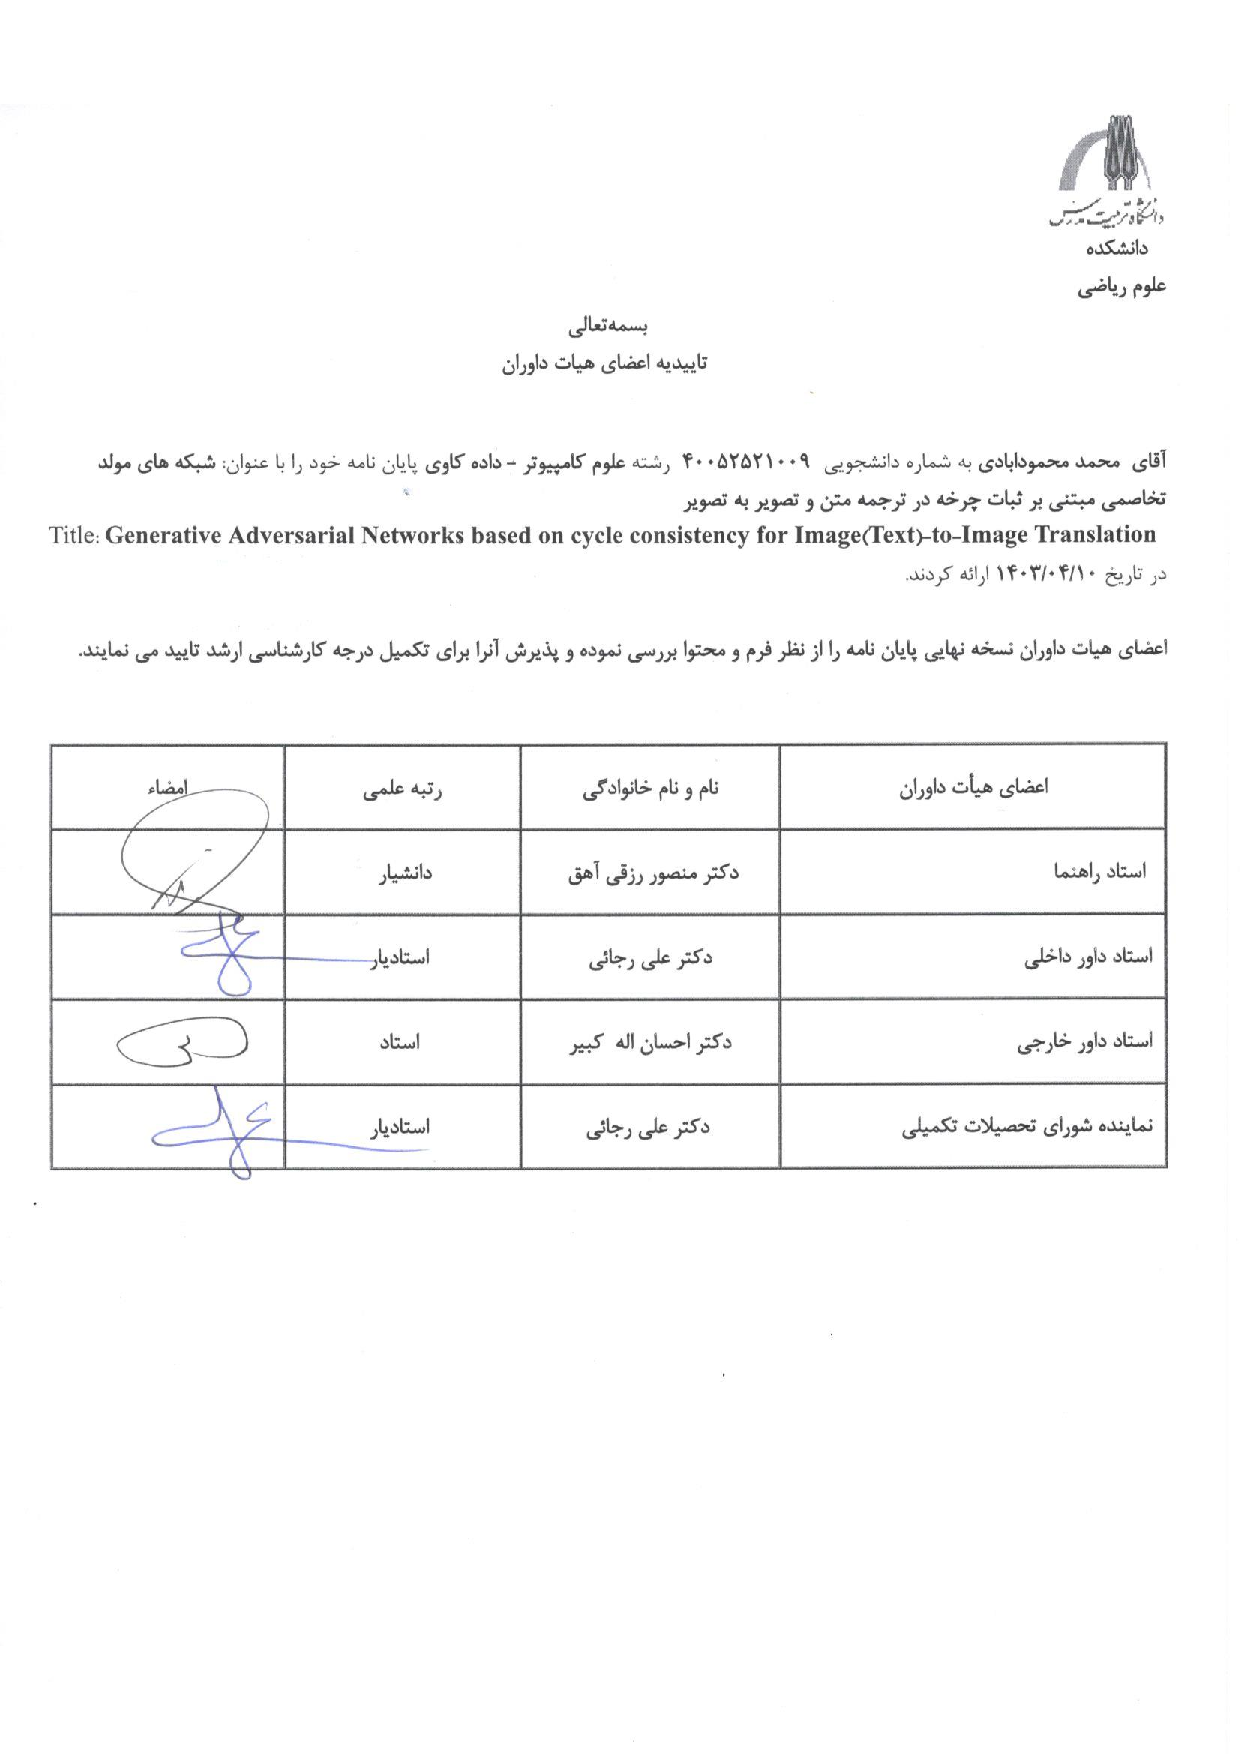
\includepdf[]{thesispage2}
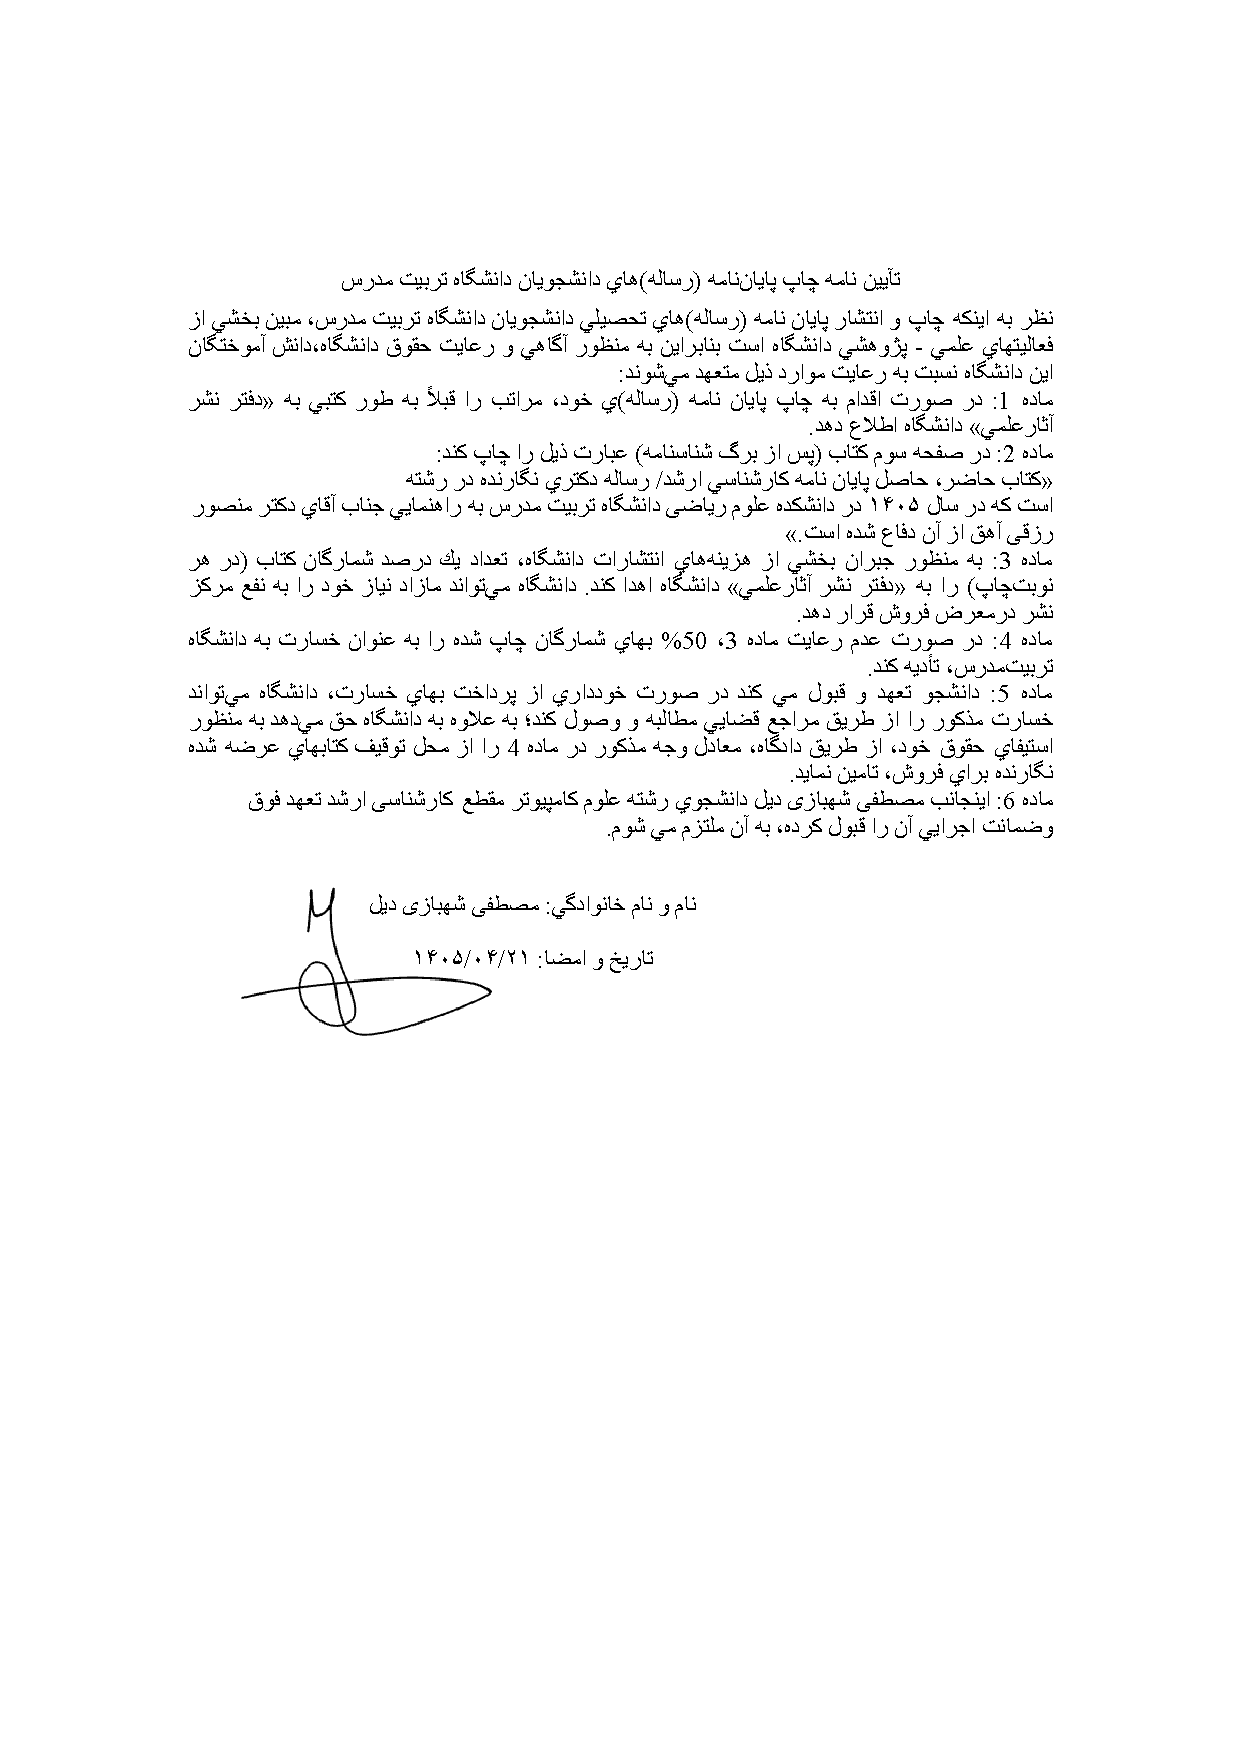
\includepdf[]{thesispage4}

\includepdf[]{thesispage3}
% در این فایل، عنوان پایان‌نامه، مشخصات خود، متن تقدیمی‌، ستایش، سپاس‌گزاری و چکیده پایان‌نامه را به فارسی، وارد کنید.
% توجه داشته باشید که جدول حاوی مشخصات پایان‌نامه/رساله و همچنین، مشخصات داخل آن، به طور خودکار، درج می‌شود.
%%%%%%%%%%%%%%%%%%%%%%%%%%%%%%%%%%%%

\thispagestyle{empty}

% \includepdf[pages=-]{firstpages.pdf}


% دانشگاه خود را وارد کنید
\university{تربیت مدرس}
% دانشکده، آموزشکده و یا پژوهشکده  خود را وارد کنید
\faculty{علوم ریاضی}
% گروه آموزشی خود را وارد کنید
\degree {کارشناسی ارشد علوم کامپیوتر گرایش داده کاوی}
% گروه آموزشی خود را وارد کنید
\subject{علوم کامپیوتر }
% گرایش خود را وارد کنید
\field{علوم کامپیوتر (داده کاوی)}
% عنوان پایان‌نامه را وارد کنید
\title{بهبود مدل‌های انتشار مبتنی بر مبدل‌های بینایی برای تولید تصویر}
% نام استاد(ان) راهنما را وارد کنید
\firstsupervisor{دکتر منصور رزقی آهق}
%\secondsupervisor{استاد راهنمای دوم}
% نام استاد(دان) مشاور را وارد کنید. چنانچه استاد مشاور ندارید، دستور پایین را غیرفعال کنید.
%\firstadvisor{نام استاد(دان) مشاور}
%نام استاد مشاور را وارد کنید. چنانچه دو استاد مشاور دارید  دستور پایین را نیز فعال کنید.
%\secondadvisor{نام استاد(دان) مشاور}
% نام پژوهشگر را وارد کنید
\name{مصطفی}
% نام خانوادگی پژوهشگر را وارد کنید
\surname{شهبازی دیل}
% تاریخ پایان‌نامه را وارد کنید
\thesisdate{بهمن ۱۴۰۴}
% کلمات کلیدی پایان‌نامه را وارد کنید
%\keywords{داده‌های بقا فضایی، مدل‌های شکنندگی فضایی}
% کلمات کلیدی پایان‌نامه را وارد کنید
\keywords{مبدل‌های بینایی، مدل‌های انتشار، ویژگی‌های محلی و سراسری، تجمیع ویژگی، تنظیم دقیق پارامتر-کارا}
\newpage
%\fa-abstract{\noindent
%در

%}
%\newpage
\thispagestyle{empty}
\vtitle
%\newpage
%\thispagestyle{empty}
%\clearpage
%~~~
%\newpage
%\thispagestyle{empty}
%\input{rights}
%\newpage
%\thispagestyle{empty}
%\clearpage
%~~~
%\newpage
%\thispagestyle{empty}
%\centerline{{\includegraphics[width=20 cm]{replyrecord}}}
%\newpage
%\thispagestyle{empty}
%\clearpage
%~~~
% \newpage
%  % پایان‌نامه خود را تقدیم کنید!
% \begin{acknowledgementpage}

% \vspace{4cm}

% {\nastaliq
% {\Large
%  تقدیم به
% \vspace{1.5cm}

% \newdimen\xa
% \xa=\textwidth
% \advance \xa by -14cm
% \hspace{\xa}
% پدر و مادر مهربانم
% \vspace{1.5cm}

% \newdimen\xa
% \xa=\textwidth
% \advance \xa by -12cm
% \hspace{\xa}
% %و زنان آزاده کشورم
% \vspace{1.5cm}

% \newdimen\xa
% \xa=\textwidth
% \advance \xa by -10cm
% \hspace{\xa}

% \vspace{1.5cm}

% \newdimen\xa
% \xa=\textwidth
% \advance \xa by -8cm
% \hspace{\xa}
% }}
% \end{acknowledgementpage}
%\newpage
%\thispagestyle{empty}
%\clearpage
%~~~
%%%%%%%%%%%%%%%%،%%%%%%%%%%%%%%%%%%%%
%\newpage
%\thispagestyle{empty}
% ستایش
%\baselineskip=.750cm
%\ \\ \\
%
%{\nastaliq
%رسيدن، به دانش است و به كردار نیک...%
%}\\
%\vspace{.5cm}\\
%{\scriptsize\nastaliq
%{
% و بی دانش به كردار نيك هم نتوان رسيد، كه نيكى را پيشتر ببايد شناختن، آنگاه بجاى آوردن. پس دانش به همه حال مى‌ببايد تا به رستگارى %توان رسيدن. و چون دانش راه آمد، به بهترين چيزها كه آدمى را تواند بودن. و در اوّل آفرينش حاصل نيست و بعضى از آن بى‌رنج و انديشه حاصل شود، پس هرآينه مهمتر چيزى باشد كه در حاصل كردنش عمر گذرانند، ليكن برخى هست كه بى‌انديشه حاصل آيد و بعضى را ناچار به انديشه حاجت بود، و آنچه به انديشه حاصل شود دانسته‌اى خواهد كه درو انديشه كنند تا اين نادانسته بدان انديشه كه در آن دانسته كنند دانسته شود، و از هر دانسته هر نادانسته را نتوان شناخت، بلكه هر نادانسته را به دانسته‌اى كه در خور او بود توان شناخت. و منطق آن علم است كه درو راه انداختن نادانسته به دانسته دانسته شود...
% }}
%
%\vspace{.5cm}
%{\nastaliq
%\newdimen\xb
%\xb=\textwidth
%\advance \xb by -8.5cm
%\hspace{\xb}
%پس منطق ناگزير آمد بر جوينده‌ی رستگاری.
%\RTLfootnote{مقدمه‌ی رساله‌ی منطق دانشنامه‌ی علائی، شیخ‌الرئیس ابن‌سینا}
%}
%\newpage
%\thispagestyle{empty}
%\clearpage
%~~~
%%%%%%%%%%%%%%%%%%%%%%%%%%%%%%%%%%%%
% \newpage
% \thispagestyle{empty}
% %قدردانی
% {\nastaliq
% قدردانی
% }
% \\[2cm]
% {\scriptsize\nastaliq
% منّت خدای را عزّ و جل که طاعتش موجب قربت است و به شکر اندرش مزید نعمت. هر نفسی که فرو می‌رود مُمِدّ حیات است و چون بر می‌آید مُفَرّح ذات. پس در هر نفسی دو نعمت موجود است و بر هر نعمتی شکری واجب(دیباچه گلستان).
% }


% % با استفاده از دستور زیر، امضای شما، به طور خودکار، درج می‌شود
% \signature
% %
\newpage
\thispagestyle{empty}
\baselineskip=1.0cm
\ \\ \\
\begin{large}
\begin{center}
چکیده
\end{center}
\end{large}
%}}
%\\[4cm]
مدل‌های انتشار مبتنی بر مبدل، مانند \lr{DiT}، کیفیت بالایی در تولید تصویر شرطی ارائه می‌کنند، اما تنظیم دقیق کامل آن‌ها برای دامنه‌ها یا نیازهای جدید از نظر حافظه، زمان آموزش و ذخیره‌سازی پرهزینه است. این پژوهش معماری \lr{DuoDiT} را برای تنظیم دقیق پارامتر-کارای مدل‌های \lr{DiT} معرفی می‌کند. در این معماری، بدنه اصلی \lr{DiT-XL/2} منجمد باقی می‌ماند و یک شاخه دوم با اندازه پچ کوچک‌تر، ویژگی‌های محلی و ریزدانه را استخراج می‌کند. برای هم‌تراز کردن این شاخه با توکن‌های بدنه اصلی، از مکانیزم توکن کلاس محلی استفاده می‌شود که هر گروه مکانی از توکن‌های ریزدانه را به‌صورت محتوا-آگاه خلاصه می‌کند. ارزیابی اصلی روی ۵۰ هزار عکس تولیده به صورت شرطی روی مجموعه داده 
\lr{ImageNet-1K}
 در وضوح 
 $256 \times 256$
   انجام شده است. نسخه 
   \lr{DuoDiT-200}
    با 
    \lr{17.95M}
     پارامتر آموزش‌پذیر از مجموع \lr{690.39M} پارامتر، به \lr{FID=2.219}، \lr{KID=0.0014} و \lr{LPIPS-Mean=0.7162} می‌رسد. همچنین در مطالعه انسانی، نمونه‌های \lr{DuoDiT} در \lr{53.26\%} مقایسه‌ها نسبت به \lr{LightningDiT} ترجیح داده شدند. نتایج نشان می‌دهد که افزودن یک مسیر سبک و وضوح‌بالا می‌تواند بدون آموزش مجدد کامل مدل، کیفیت ادراکی و کارایی تنظیم دقیق را بهبود دهد.\\
\textit{ \textbf{ واژه‌های کلیدی:}}
مبدل‌های بینایی، مدل‌های انتشار، ویژگی‌های محلی و سراسری، تجمیع ویژگی، تنظیم دقیق پارامتر-کارا.
%\newpage
%\thispagestyle{empty}
%\clearpage
%~~~
%\newpage
%{\small
%\abstractview
%}
%\newpage
%\thispagestyle{empty}
%\clearpage
%~~~
\newpage

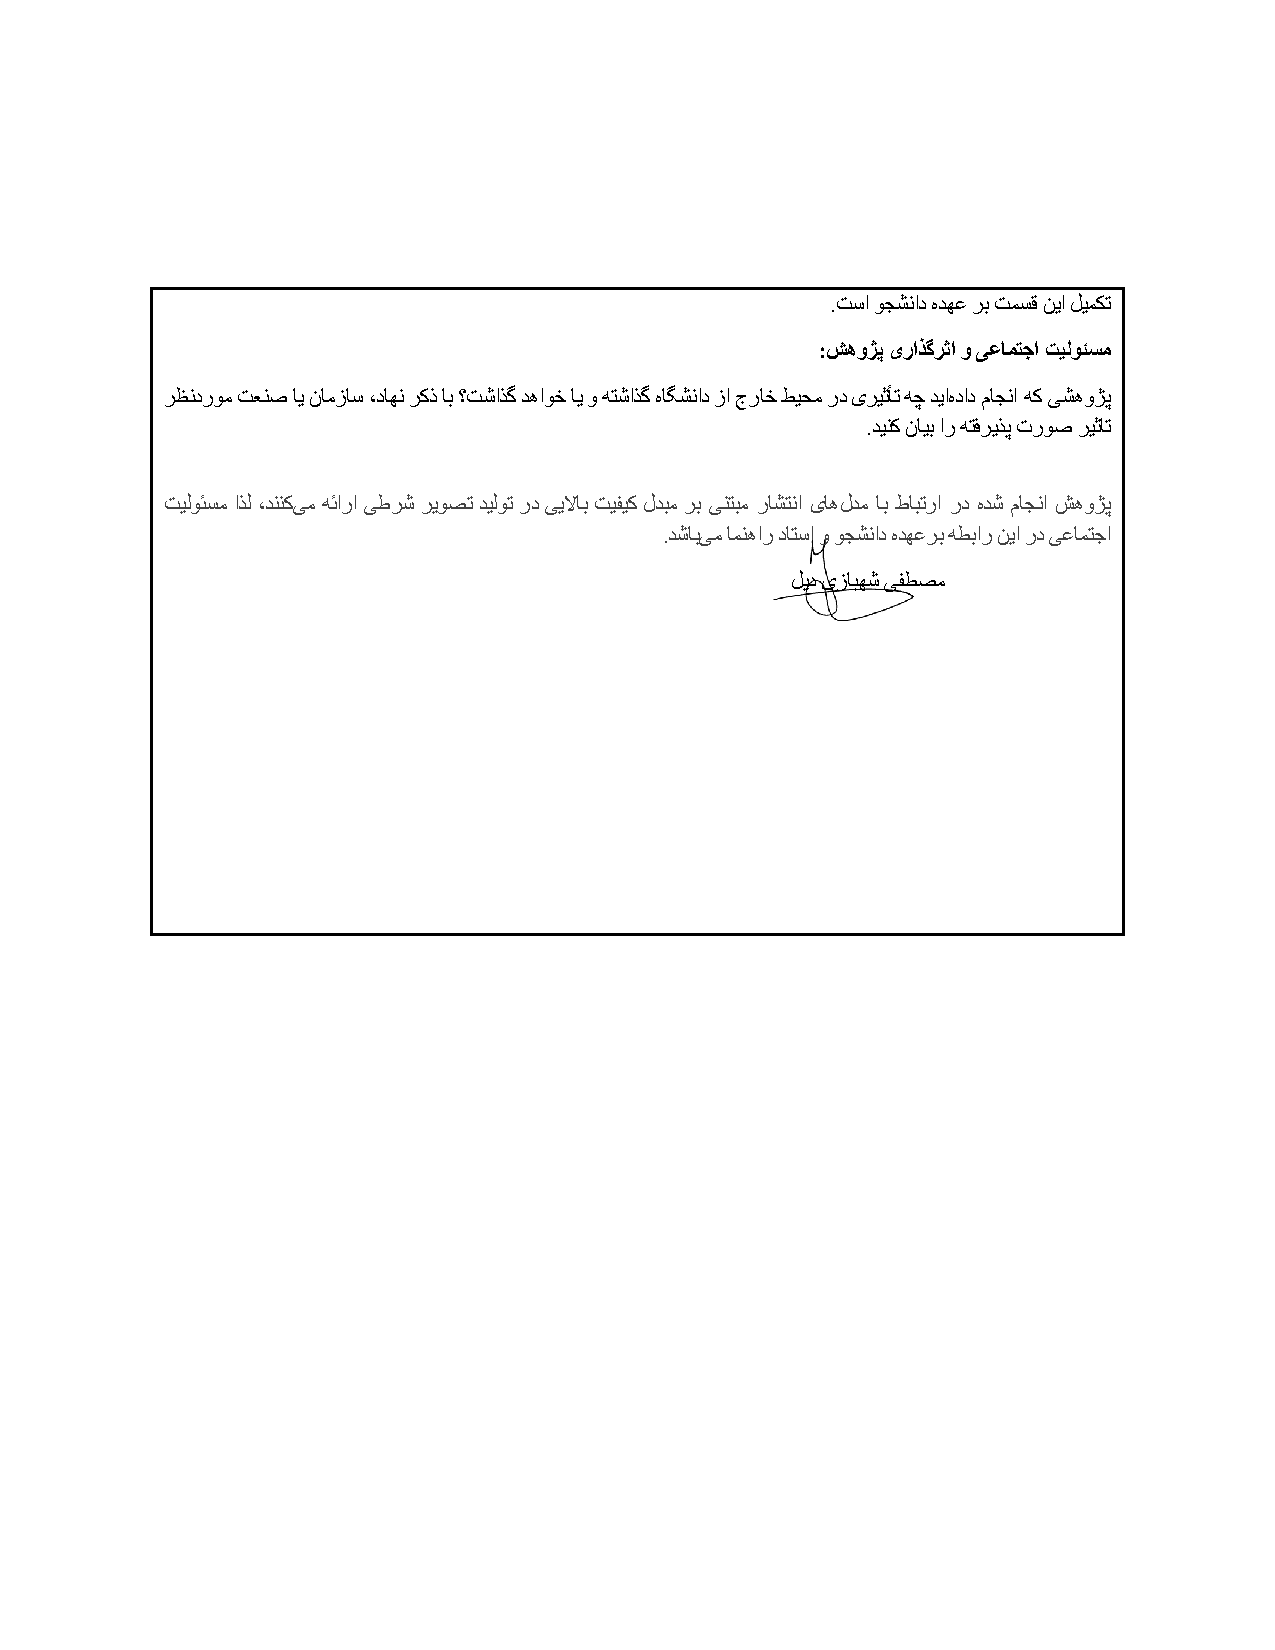
\includepdf[]{Tassir}
\label{footdir@1}
\label{footdir@2}
\label{footdir@3}
%\pagenumbering{harfi}
% \includepdf[]{Taasir}
\pagenumbering{alph}
\tableofcontents
\listoftables
\listoffigures
\clearpage{\pagestyle{empty}\cleardoublepage}

\baselineskip=1.0cm
\chapter*{پیشگفتار}
\phantomsection%
\addcontentsline{toc}{chapter}{پیشگفتار}%
\markboth{پیشگفتار}{پیشگفتار}
\label{sec:preface}

یادگیری ماشین به عنوان یکی از ارکان بنیادین هوش مصنوعی مدرن، در دهه‌های اخیر پیشرفت‌های مهمی را در نحوه تعامل سامانه‌های محاسباتی با داده‌ها رقم زده است. این شاخه از علم که بر آماره، بهینه‌سازی و یادگیری از نمونه‌ها استوار است، به سیستم‌ها امکان می‌دهد الگوهای پنهان را بدون طراحی صریح همه قواعد تصمیم‌گیری استخراج کنند \cite{726791,Vaswani2017}. با افزایش حجم داده‌ها و توان محاسباتی، یادگیری عمیق به چارچوب غالب بسیاری از کاربردهای هوش مصنوعی تبدیل شد و شبکه‌های عصبی عمیق توانستند در حوزه‌هایی مانند پردازش زبان طبیعی، تشخیص گفتار و بینایی ماشین عملکردی بسیار رقابتی ارائه دهند \cite{Vaswani2017,Dosovitskiy2020}. در بینایی ماشین، موفقیت شبکه‌های عصبی پیچشی در استخراج ویژگی از تصویر، نقطه شروع مهمی برای توسعه سامانه‌های دیداری مدرن بود و بعدها معماری‌های مبتنی بر مبدل نیز این مسیر را گسترش دادند \cite{726791,Dosovitskiy2020}.

بینایی ماشین، به عنوان یکی از مسیرهای اصلی کاربرد هوش مصنوعی در داده‌های بصری، از وظایف تحلیلی مانند طبقه‌بندی تصویر و تشخیص اشیا به سمت وظایف مولد نیز گسترش یافته است \cite{5206848,chen2025diffusionImageGenerationSurvey}. مدل‌های مولد نه تنها محتوای بصری را بازنمایی می‌کنند، بلکه می‌توانند نمونه‌های جدیدی مشابه توزیع داده‌های واقعی تولید کنند؛ این مسیر ابتدا با خانواده‌هایی مانند خودکدگذارهای تغییرپذیر\LTRfootnote{Variational Autoencoders} (\lr{VAE}) و شبکه‌های مولد تخاصمی\LTRfootnote{Generative Adversarial Networks} (\lr{GAN}) شکل گرفت و سپس با مدل‌های انتشار احتمالی به سطح تازه‌ای از کیفیت و پایداری رسید \cite{Kingma2013,Goodfellow2014,0214306}. مدل‌های انتشار با فرمول‌بندی تولید تصویر به عنوان وارون‌سازی تدریجی فرآیند نویزدهی، در بسیاری از وظایف تولید تصویر کیفیت و تنوع بالایی نشان داده‌اند و در مقایسه با \lr{GAN}ها از پایداری آموزشی مناسب‌تری برخوردارند \cite{8567753,chen2025diffusionImageGenerationSurvey}.

ترکیب مدل‌های انتشار با معماری‌های مبدل، به‌ویژه مبدل بینایی\LTRfootnote{Vision Transformer} (\lr{ViT})، مسیر شکل‌گیری مدل‌های مولد مقیاس‌پذیر را تقویت کرده است \cite{Dosovitskiy2020,2212.09748}. معماری‌هایی مانند \lr{DiT} با استفاده از بلوک‌های مبدل و سازوکارهایی مانند \lr{adaLN-Zero} برای شرط‌گذاری زمانی و کلاسی، نشان داده‌اند که افزایش ظرفیت و محاسبات می‌تواند کیفیت تولید تصویر را بهبود دهد \cite{2212.09748}. با این حال، استفاده از این مدل‌های بزرگ در دامنه‌های خاص، تنظیم دقیق کامل همه پارامترها (\lr{Full Fine-Tuning})، حافظه گرافیکی زیاد، زمان آموزش طولانی و ذخیره نسخه‌های متعدد از مدل را به مسئله‌ای پرهزینه تبدیل می‌کند \cite{5294562,8409325}.

در پاسخ به این چالش، روش‌های تنظیم دقیق پارامتر-کارا\LTRfootnote{Parameter-Efficient Fine-Tuning} توسعه یافته‌اند تا تنها بخش کوچکی از پارامترها برای سازگار کردن مدل با وظیفه جدید آموزش داده شود \cite{2479204,8409325}.
. با این حال، اگر تغییرات فقط در همان وضوح توکنی فشرده بدنه اصلی اعمال شوند، ممکن است بازسازی جزئیات مکانی و مؤلفه‌های فرکانس بالا محدود بماند. این مسئله انگیزه‌ای برای طراحی شاخه‌هایی است که بتوانند با وضوح مکانی بالاتر ویژگی‌های محلی را استخراج کنند و در عین حال بدنه اصلی مدل را ثابت نگه دارند \cite{wang2020hrnet,chen2021crossvit}.

یکی از راهکارهای مناسب برای این هدف، تفکیک وظایف «درک معنایی» و «حفظ جزئیات» در قالب معماری دوجریانی (\lr{Dual-Stream Architecture}) است \cite{wang2020hrnet,chen2021crossvit}. در این دیدگاه، جریان اصلی می‌تواند ساختار کلی و مفاهیم سطح بالا را حفظ کند، در حالی که جریان موازی کم‌هزینه روی جزئیات ریزدانه و ویژگی‌های فرکانس بالا تمرکز دارد \cite{wang2020hrnet}. چالش اصلی چنین طراحی‌ای، همگام‌سازی و ادغام کنترل‌شده اطلاعات جریان فرعی با بدنه اصلی است تا فرآیند تولید تصویر از نظر معنایی و مکانی منسجم باقی بماند \cite{chen2021crossvit,2209.12152}.

ترکیب هدفمند دو جریان نیازمند راهبردهایی فراتر از جمع ساده ویژگی‌هاست، زیرا خروجی شاخه وضوح‌بالا باید پیش از ادغام با جریان اصلی از نظر طول توالی و فضای ویژگی هم‌راستا شود \cite{chen2021crossvit,2209.12152}. استفاده از توجه متقاطع یا توکن‌های خلاصه‌ساز، از جمله توکن کلاس محلی، می‌تواند نقش یک واسط فشرده میان اطلاعات محلی و بازنمایی سراسری را ایفا کند \cite{Dosovitskiy2020,chen2021crossvit}. چنین سازوکاری به مدل اجازه می‌دهد در عین حفظ دانش کلی بدنه اصلی، اطلاعات ریزدانه و مکانی را نیز به‌صورت کنترل‌شده وارد فرآیند تولید کند \cite{2212.09748,2209.12152}.

علاوه بر ارتقای کیفیت بصری، منجمد نگه داشتن بخش اعظم شبکه و آموزش تنها شاخه کمکی می‌تواند فشار حافظه، تعداد پارامترهای آموزش‌پذیر و هزینه ذخیره مدل را کاهش دهد \cite{2479204,8409325}. این ویژگی برای کاربردهایی که نیازمند تنظیم دقیق سریع، شخصی‌سازی یا سازگاری با دامنه جدید هستند اهمیت ویژه‌ای دارد، زیرا امکان بهره‌گیری از \lr{Large Diffusion Models} را بدون آموزش مجدد کامل فراهم می‌کند \cite{ryu2023loradiffusion,0052338,2755774}. بنابراین، طراحی یک مسیر کمکی سبک در کنار بدنه اصلی منجمد، از نظر محاسباتی و کاربردی با جهت‌گیری پژوهش‌های اخیر در مدل‌های مولد همسو است \cite{2212.09748,8409325}.

در نهایت، تمرکز اصلی این پایان‌نامه بر اعمال تغییرات معماری هدفمند در مدل \lr{DiT} است تا تنظیم دقیق پارامتر-کارا با حفظ جزئیات محلی ممکن شود \cite{2212.09748,8409325}. بر اساس معماری نهایی پیاده‌سازی‌شده، یک شاخه موازی تحت عنوان $x2$ به شبکه افزوده می‌شود که ویژگی‌های مکمل را با وضوح مکانی بالاتر استخراج می‌کند و سپس از طریق توکن‌های کلاس محلی با جریان اصلی هم‌راستا و ادغام می‌شود \cite{chen2021crossvit,2088740}. ارزیابی این پژوهش روی تولید شرطی \lr{ImageNet-1K} نشان می‌دهد که \lr{DuoDiT-200} با آموزش \lr{17.95M} پارامتر از مجموع \lr{690.39M} پارامتر، به \lr{FID=2.219}، \lr{KID=0.0014} و \lr{LPIPS-Mean=0.7162} می‌رسد. این طراحی با منجمد نگه داشتن بدنه اصلی (\lr{Frozen Backbone})، امکان بهره‌گیری از دانش پیش‌آموزش‌دیده را حفظ می‌کند و هم‌زمان مسیر سبک‌تری برای سازگاری با داده‌ها یا کلاس‌های هدف فراهم می‌آورد \cite{2212.09748,Pan2024FineDiffusion}.

\clearpage{\pagestyle{empty}\cleardoublepage}

\pagenumbering{arabic}
{
\chapter{مفاهیم اولیه}
\label{chp1}

تولید تصویر\LTRfootnote{Image Generation} یکی از مفاهیم پایه‌ای مدل‌سازی مولد است و به یادگیری توزیع داده‌های تصویری و نمونه‌برداری از آن برای ساخت تصاویر جدید، طبیعی و معنادار اشاره دارد؛ به‌گونه‌ای که تصویر تولیدشده از نظر ساختار، محتوا و جزئیات بصری به نمونه‌های واقعی شباهت داشته باشد \cite{chen2025diffusionImageGenerationSurvey,0214306}. این مسئله در حالت پایه معمولاً ماهیتی بی‌ناظر یا خودنظارتی دارد، زیرا هدف مدل، یادگیری الگوهای پنهان موجود در مجموعه‌ای از تصاویر بدون نیاز به برچسب‌گذاری کامل برای هر ویژگی بصری است؛ هرچند در بسیاری از کاربردها می‌توان با افزودن شرط‌هایی مانند برچسب کلاس، متن یا تصویر راهنما، فرآیند تولید را کنترل کرد \cite{8567753,9851474}. بر همین اساس، تعریف تولید تصویر نیز بخشی از مفاهیم اولیه این فصل است و در ادامه، برای فراهم شدن زمینه معرفی معماری پیشنهادی، معماری‌های بنیادی یادگیری عمیق، مدل‌های مولد شامل خودکدگذارهای تغییرپذیر، شبکه‌های مولد تخاصمی و مدل‌های انتشار، مبدل‌ها، مبدل‌های بینایی، مجموعه‌داده مورد استفاده و معیارهای ارزیابی مرور می‌شوند \cite{Kingma2013,Goodfellow2014,chen2025diffusionImageGenerationSurvey}.

\section{شبکه‌های عصبی پیچشی (\lr{CNN})}
\label{sec:ch1-cnn}
شبکه‌های عصبی پیچشی\LTRfootnote{Convolutional Neural Networks} یکی از مهم‌ترین معماری‌های یادگیری عمیق هستند که به‌طور خاص برای پردازش داده‌های دارای ساختار شبکه‌ای، مانند تصاویر، طراحی شده‌اند. ایده اصلی این شبکه‌ها الهام‌گرفته از سیستم بینایی بیولوژیکی است و بر پایه عملیات ریاضی «پیچش» بنا شده است \cite{726791}.
در این شبکه‌ها، به جای اتصال تمام نورون‌ها به هم (مانند شبکه‌های تمام‌متصل)، از فیلترها (کرنل‌ها) برای استخراج ویژگی‌های محلی استفاده می‌شود. این فیلترها روی تصویر ورودی لغزیده و ویژگی‌های مختلفی مانند لبه‌ها، بافت‌ها و الگوهای پیچیده‌تر را در لایه‌های عمیق‌تر شناسایی می‌کنند. دو مفهوم کلیدی در این معماری‌ها وجود دارد. نخست، «اشتراک وزن»\LTRfootnote{Weight Sharing} که در آن تمام نورون‌های یک نقشه ویژگی\LTRfootnote{Feature Map} از فیلتر یکسانی استفاده می‌کنند و باعث کاهش چشمگیر تعداد پارامترها و ایجاد خاصیت تغییرناپذیری نسبت به انتقال\LTRfootnote{Translation Invariance} می‌شود. دوم، استفاده از «لایه‌های تجمیع»\LTRfootnote{Pooling Layer} است که ابعاد مکانی ویژگی‌ها را کاهش می‌دهند\LTRfootnote{Max Pooling} تا هم محاسبات سبک‌تر شود و هم شبکه نسبت به تغییرات جزئی مکان ویژگی‌ها مقاوم‌تر گردد \cite{726791}.

\section{خودکدگذارهای تغییرپذیر (\lr{VAE})}
\label{sec:ch1-vae}
خودکدگذارهای تغییرپذیر 
(\lr{VAE})
 دسته‌ای از مدل‌های مولد احتمالی هستند که بر خلاف خودکدگذارهای معمولی که ورودی را به یک نقطه ثابت در فضای نهان نگاشت می‌کنند، آن را به یک توزیع احتمالی (معمولاً توزیع نرمال) نگاشت می‌نمایند \cite{Kingma2013}.
معماری \lr{VAE} شامل دو بخش اصلی است. بخش اول، «رمزگذار»\LTRfootnote{Encoder} است که یک شبکه عصبی احتمالی $q_\phi(z|x)$ بوده و پارامترهای توزیع نهان (میانگین $\mu$ و واریانس $\sigma^2$) را برای ورودی $x$ پیش‌بینی می‌کند. بخش دوم، «رمزگشا»\LTRfootnote{Decoder} با توزیع $p_\theta(x|z)$ است که تلاش می‌کند داده ورودی را با نمونه‌برداری از فضای نهان $z$ بازسازی کند. هدف آموزش در این مدل‌ها، بیشینه‌سازی کران پایین شواهد\LTRfootnote{Evidence Lower Bound - ELBO} است که شامل دو مؤلفه اصلی می‌شود؛ خطای بازسازی که باعث شباهت خروجی به ورودی شده، و واگرایی کولبک-لایبلر\LTRfootnote{KL Divergence} که تضمین می‌کند توزیع فضای نهان به توزیع پیشین (معمولاً نرمال استاندارد) نزدیک بماند تا امکان تولید نمونه‌های جدید فراهم گردد \cite{Kingma2013}.

\begin{equation}
    \mathcal{L}_{\text{ELBO}} = \mathbb{E}_{q_\phi(z|x)}[\log p_\theta(x|z)] - D_{KL}(q_\phi(z|x) \| p(z))
\end{equation}

\section{شبکه‌های مولد تخاصمی (\lr{GAN})}
\label{sec:ch1-gan}
شبکه‌های مولد تخاصمی (\lr{GAN}) که توسط گودفلو و همکاران معرفی شدند، رویکردی متفاوت برای تولید داده دارند که مبتنی بر تئوری بازی‌هاست \cite{Goodfellow2014}. این مدل از دو شبکه عصبی تشکیل شده است که در یک بازی مجموع‌صفر با هم رقابت می‌کنند. شبکه اول، «مولد»\LTRfootnote{Generator - $G$} نام دارد و سعی می‌کند داده‌های مصنوعی تولید کند که تا حد ممکن شبیه به داده‌های واقعی باشند تا رقیب خود را فریب دهد. شبکه دوم، «متمایزگر»\LTRfootnote{Discriminator - $D$} است که وظیفه دارد تشخیص دهد که داده ورودی، واقعی (از مجموعه‌داده) است یا جعلی (تولید شده توسط $G$). تابع هدف این بازی به صورت زیر تعریف می‌شود:
\begin{equation}
    \min_G \max_D V(D, G) = \mathbb{E}_{x \sim p_{\text{data}}(x)}[\log D(x)] + \mathbb{E}_{z \sim p_{z}(z)}[\log(1 - D(G(z)))]
\end{equation}
در حالی که \lr{GAN}ها قادر به تولید تصاویر با کیفیت بسیار بالا هستند، آموزش آن‌ها اغلب ناپایدار بوده و با مشکلاتی نظیر فروپاشی مود\LTRfootnote{Mode Collapse} مواجه می‌شوند \cite{Goodfellow2014,8567753}.

\section{مدل‌های انتشار (\lr{Diffusion Models})}
\label{sec:ch1-diffusion_models}
مدل‌های انتشار به عنوان یکی از پیشرفته‌ترین چارچوب‌های تولید داده در سال‌های اخیر شناخته می‌شوند و اساس کار آن‌ها بر شبیه‌سازی یک فرایند تبدیل تدریجی نویز تصادفی به داده منسجم مبتنی است \cite{7811582}.

\subsection{فرآیند انتشار و معادلات}
\begin{figure}[H]
    \centering
    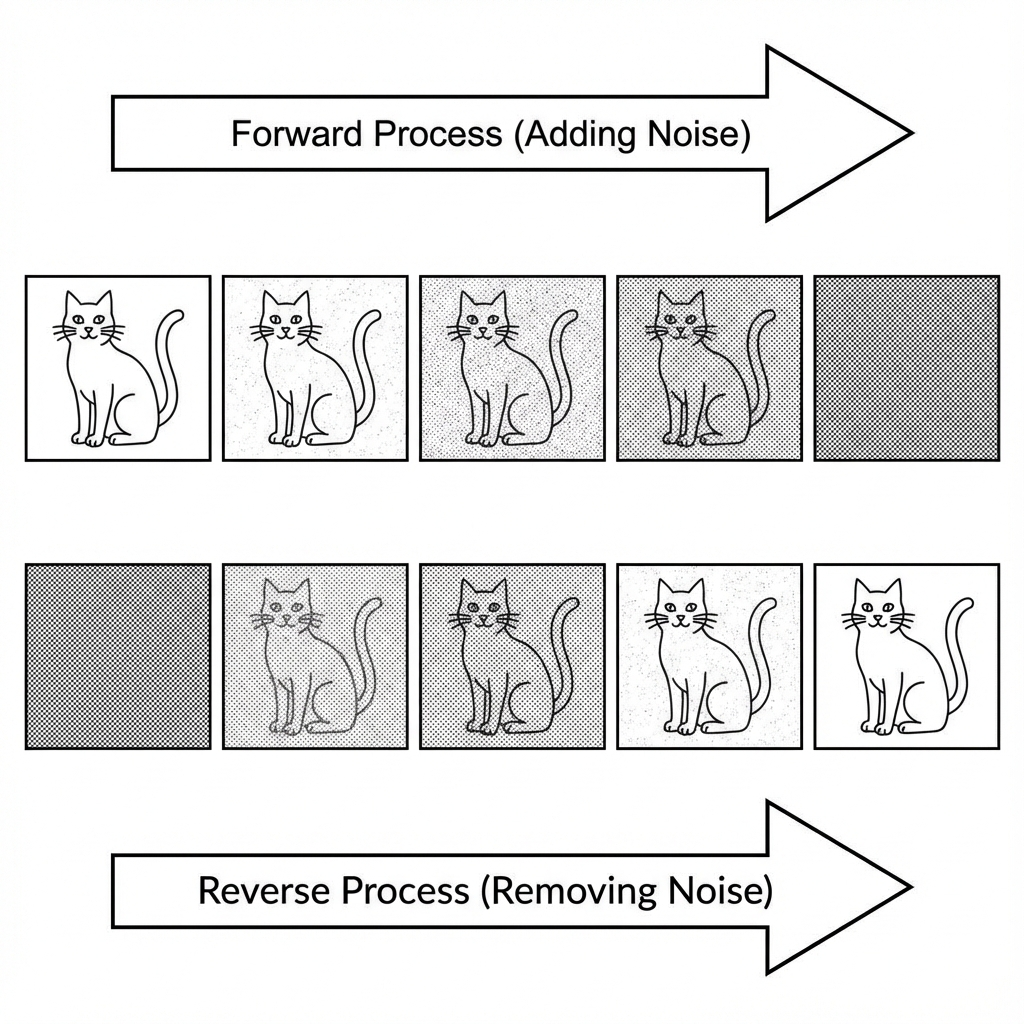
\includegraphics[width=0.9\linewidth]{images/placeholder_diffusion.png}
    \caption[شمای کلی فرآیند انتشار]{شمای کلی فرآیند انتشار: مسیر رو به جلو (افزودن نویز) و مسیر معکوس (حذف نویز).}
    \label{fig:diffusion_process}
\end{figure}
همان‌طور که در شکل \ref{fig:diffusion_process} نشان داده شده است، این سازوکار شامل دو مسیر مجزا است. نخست، «مسیر انتشار رو به جلو»\LTRfootnote{Forward Process} که طی آن نویز گاوسی به صورت تدریجی در $T$ مرحله به داده افزوده می‌شود تا جایی که داده عملاً به نویز خالص تبدیل شود. این فرآیند معمولاً به صورت یک زنجیره مارکوف با توزیع شرطی گاوسی $q(x_t|x_{t-1})$ مدل می‌شود. دوم، «مسیر انتشار معکوس»\LTRfootnote{Reverse Process} است که هدف اصلی مدل محسوب می‌شود و باید فرآیند افزوده شدن نویز را معکوس کند، یعنی $p_\theta(x_{t-1}|x_t)$. در این مرحله، یک شبکه عصبی (مانند \lr{U-Net}) برای پیش‌بینی نویز اضافه شده در هر گام زمانی آموزش می‌بیند \cite{0214306,chen2025diffusionImageGenerationSurvey}.

فرمول کلی فرآیند تصادفی پیوسته در مدل‌های انتشار را می‌توان با معادله دیفرانسیل تصادفی\LTRfootnote{SDE} توصیف کرد:
\[ \mathrm{d}x = f(t, x) \, \mathrm{d}t + \sigma(t) \, \mathrm{d}\omega \]
که در آن $f(t, x)$ ضریب رانش و $\sigma(t)$ ضریب نفوذ است. برای تولید نمونه، مدل باید تابع نمره\LTRfootnote{Score Function} یا گرادیان لگاریتم چگالی داده را تخمین بزند \cite{0214306}.


% Figure moved here to avoid floating into Section 1.5
در کنار مدل‌های پایه احتمالی\LTRfootnote{DDPM}، نسخه‌های توسعه‌یافته‌ای نظیر \lr{DDIM} برای نمونه‌برداری قطعی و سریع‌تر، و مدل‌های انتشار در فضای نهان\LTRfootnote{Latent Diffusion Models} برای کاهش بار محاسباتی معرفی شده‌اند \cite{2088740}.

\section{شبکه‌های عصبی بازگشتی (\lr{RNN})}
\label{sec:ch1-rnn}
شبکه‌های عصبی بازگشتی\LTRfootnote{Recurrent Neural Networks} برای پردازش داده‌های متوالی (مانند متن، صوت یا سری‌های زمانی) توسعه یافته‌اند. ویژگی متمایز \lr{RNN} وجود حلقه‌های بازخوردی است که به شبکه اجازه می‌دهد اطلاعات مراحل قبلی زمان ($t-1$) را در قالب یک «حالت پنهان»\LTRfootnote{Hidden State} حفظ کرده و در پردازش ورودی فعلی ($x_t$) استفاده کند \cite{rumelhart1986learning}.
معادله به‌روزرسانی حالت پنهان $h_t$ به صورت کلی برابر است با:
\begin{equation}
    h_t = f(W_h h_{t-1} + W_x x_t + b)
\end{equation}
اگرچه \lr{RNN}ها، مطابق ساختار نمایش داده‌شده در شکل \ref{fig:ch1-rnn-arch}، برای داده‌های متوالی مناسب هستند، اما در یادگیری وابستگی‌های طولانی‌مدت دچار مشکل «محو شدن گرادیان»\LTRfootnote{Vanishing Gradient} می‌شوند که مانع از انتقال موثر اطلاعات در طول توالی‌های طولانی می‌گردد \cite{hochreiter1997lstm,Vaswani2017}.

\begin{figure}[H]
    \centering
    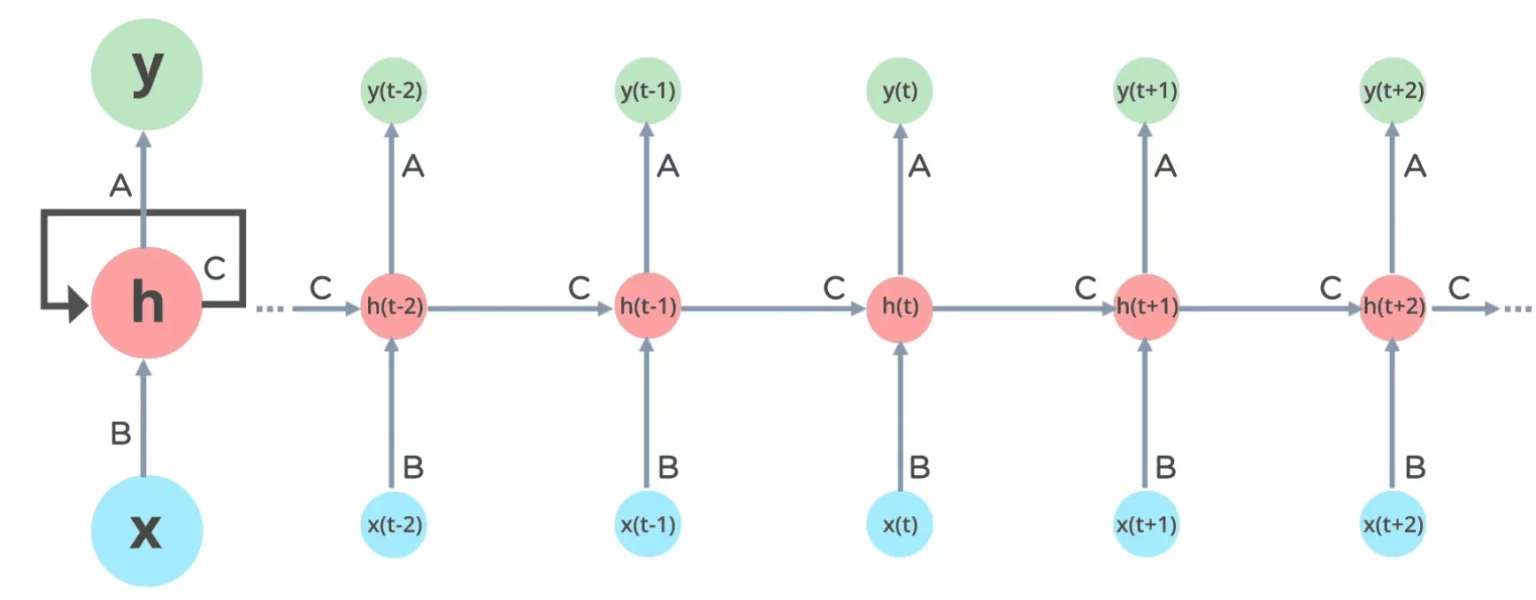
\includegraphics[width=0.9\linewidth]{images/rnn.png}
\caption[معماری شبکه عصبی بازگشتی]{معماری شبکه عصبی بازگشتی (\lr{RNN}) و نحوه باز شدن آن در طول زمان.}
    \label{fig:ch1-rnn-arch}
\end{figure}

برای حل مشکل حافظه کوتاه‌مدت در \lr{RNN}های ساده، معماری \lr{LSTM}\LTRfootnote{Long Short-Term Memory} معرفی شد که ساختار داخلی آن در شکل \ref{fig:ch1-lstm-arch} آمده است. این معماری با معرفی یک «سلول حافظه»\LTRfootnote{Cell State} و مکانیزم‌های کنترلی به نام «دروازه»\LTRfootnote{Gate}، جریان اطلاعات را دقیق‌تر مدیریت می‌کند. یک واحد \lr{LSTM} استاندارد شامل سه دروازه اصلی است. «دروازه فراموشی»\LTRfootnote{Forget Gate} تصمیم می‌گیرد چه اطلاعاتی از حافظه دور ریخته شود. سپس «دروازه ورودی»\LTRfootnote{Input Gate} مشخص می‌کند چه اطلاعات جدیدی باید در حافظه ذخیره شود و در نهایت «دروازه خروجی»\LTRfootnote{Output Gate} تعیین می‌کند چه بخشی از حافظه به عنوان خروجی لحظه‌ای ارسال گردد. این ساختار به \lr{LSTM} اجازه می‌دهد تا وابستگی‌های زمانی طولانی‌تری را نسبت به \lr{RNN} معمولی مدل کند \cite{hochreiter1997lstm}.

\begin{figure}[H]
    \centering
    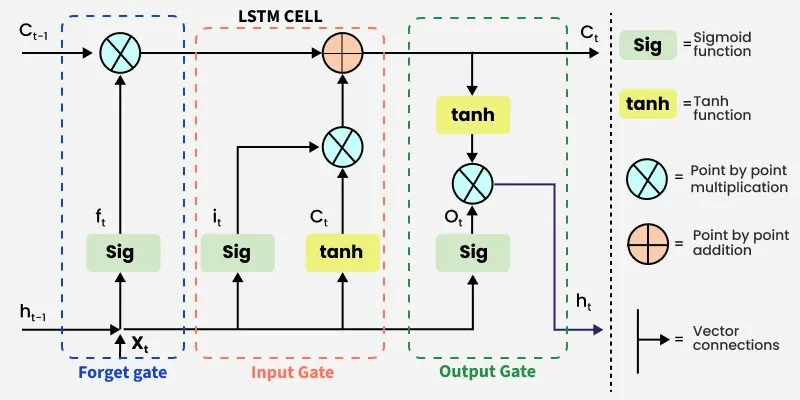
\includegraphics[width=0.9\linewidth]{images/lstm.png}
    \caption[ساختار داخلی واحد \lr{LSTM}]{ساختار داخلی یک واحد \lr{LSTM} شامل دروازه‌های فراموشی، ورودی و خروجی.}
    \label{fig:ch1-lstm-arch}
\end{figure}

\section[مبدل‌ها]{مبدل‌ها\LTRfootnote{Transformers}}
\label{sec:ch1-transformers}
معماری مبدل که ساختار کلی آن در شکل \ref{fig:ch1-transformers-arch} نمایش داده شده است، اولین بار در مقاله «توجه تمام چیزی است که نیاز دارید» معرفی شد و پارادایم پردازش توالی‌ها را تغییر داد \cite{Vaswani2017}. برخلاف \lr{RNN}ها که داده‌ها را به صورت ترتیبی پردازش می‌کنند، مبدل‌ها با استفاده از مکانیزم «توجه»\LTRfootnote{Attention} امکان پردازش موازی کل توالی را فراهم می‌کنند.

\begin{figure}[H]
    \centering
    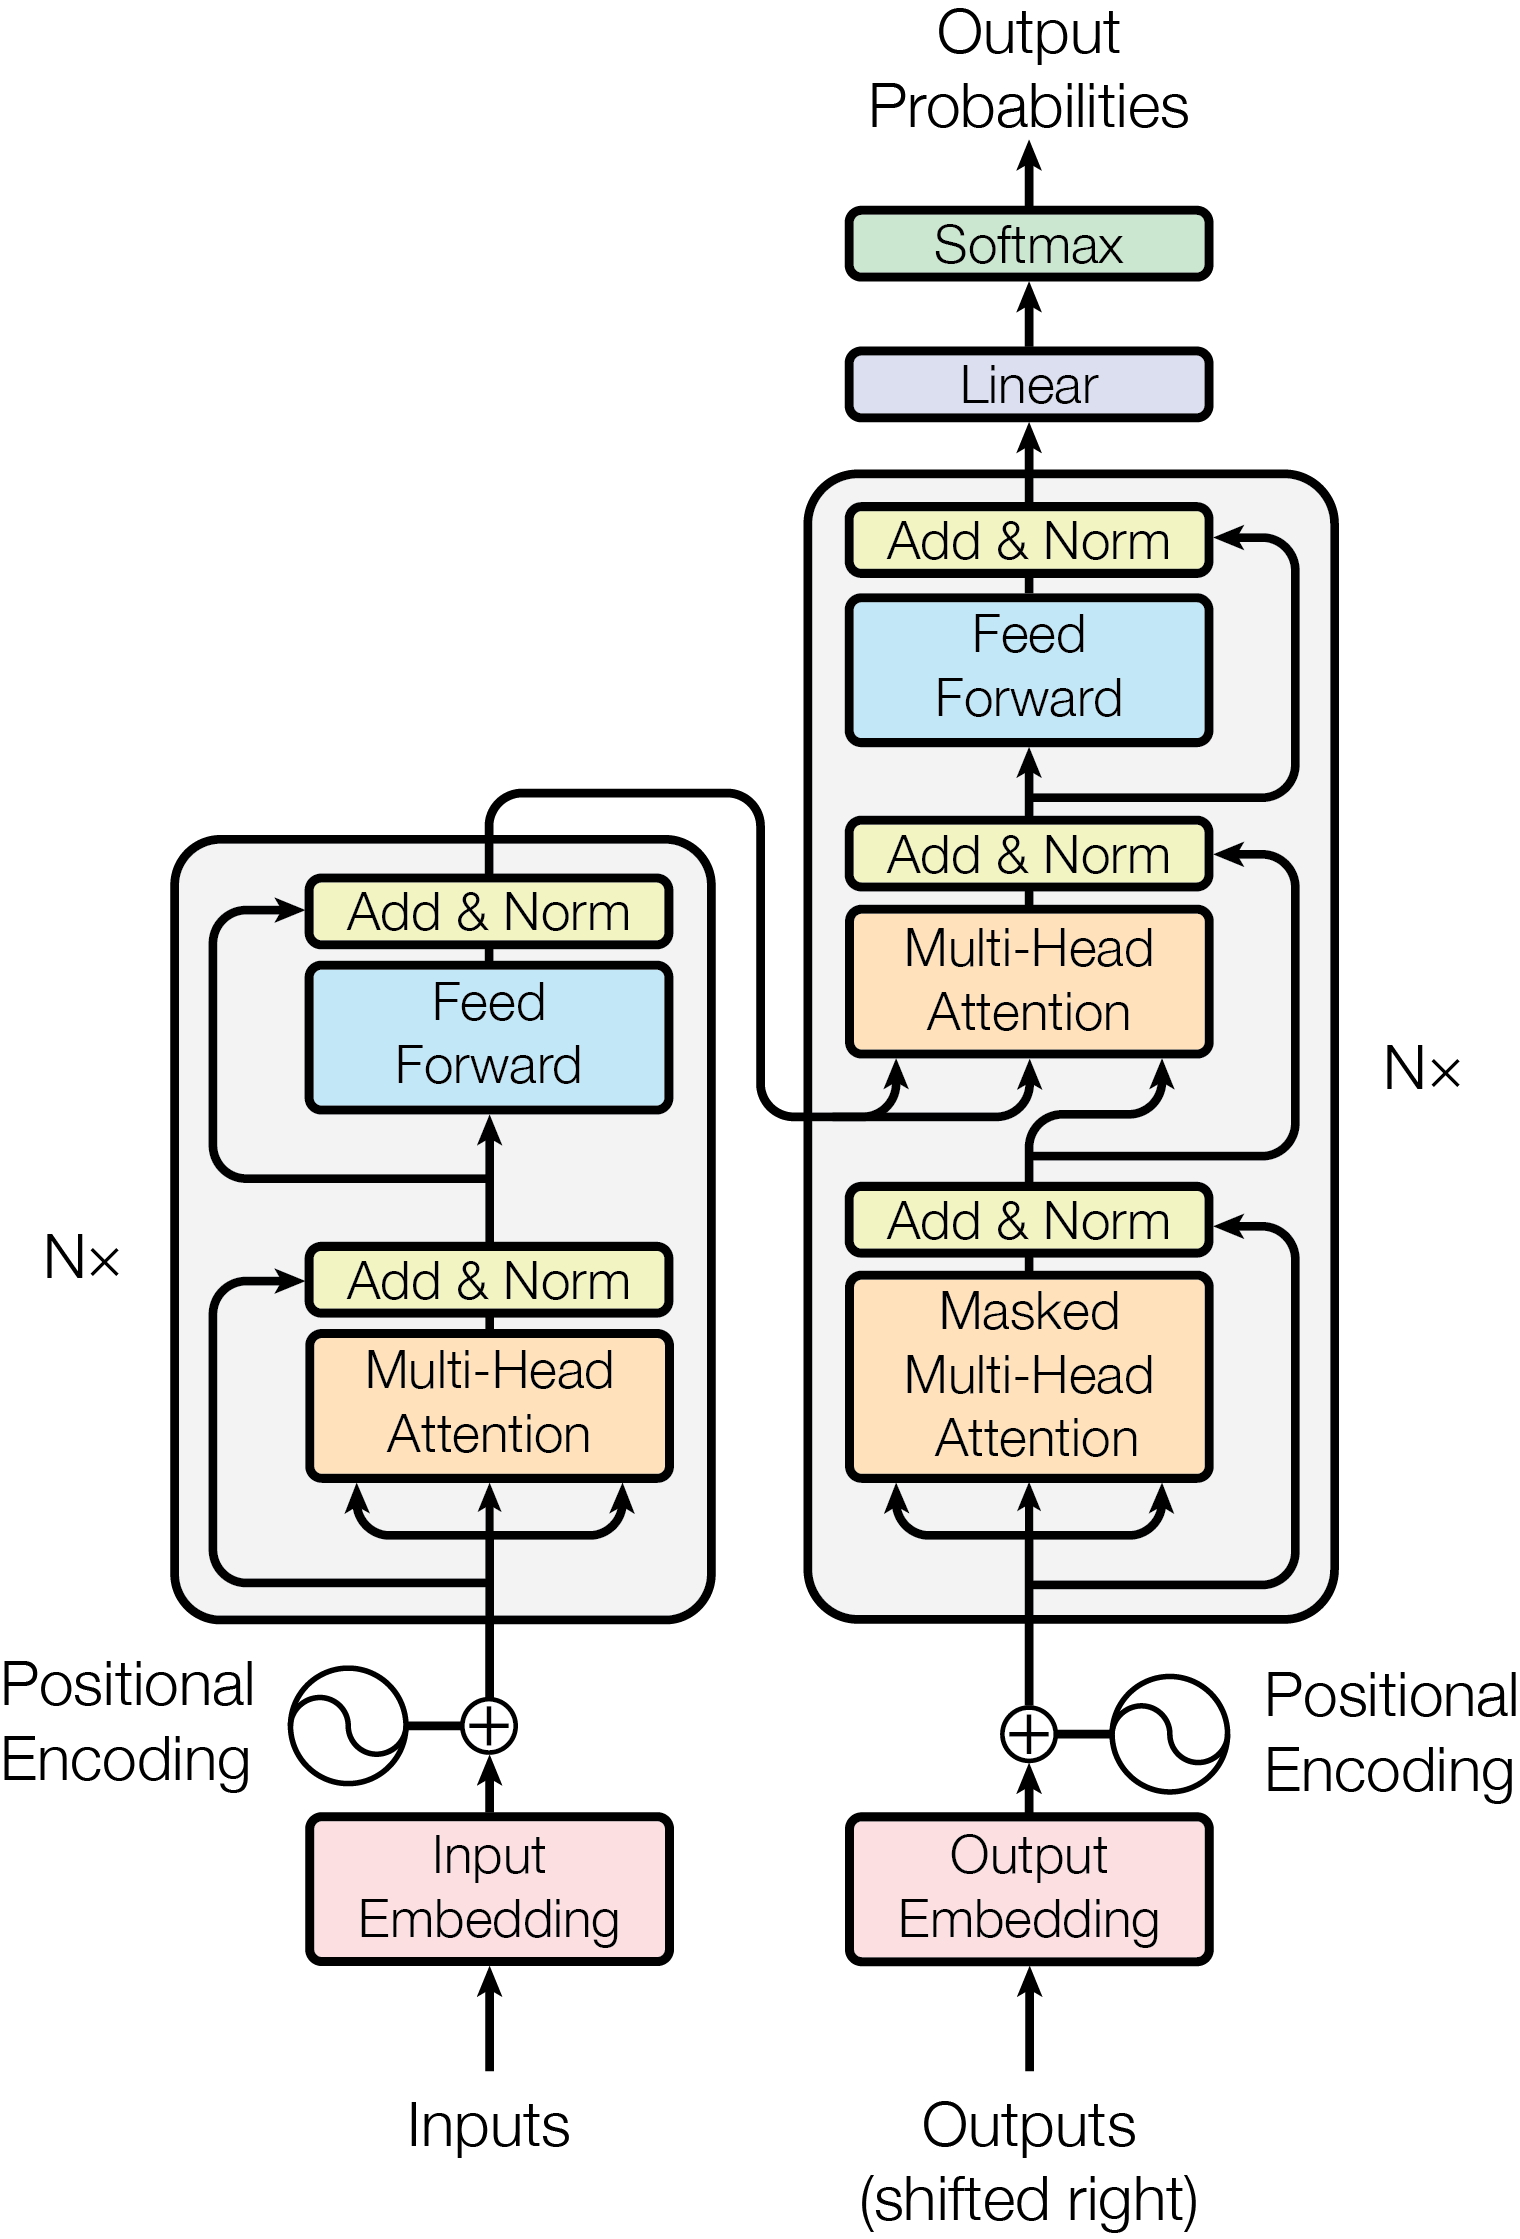
\includegraphics[width=0.9\linewidth]{images/transformers.png}
    \caption[ساختار کلی معماری مبدل]{ساختار کلی معماری مبدل شامل رمزگذار و رمزگشا.}
    \label{fig:ch1-transformers-arch}
\end{figure}

\subsection[مکانیزم توجه]{مکانیزم توجه\LTRfootnote{Attention Mechanism}}
مؤلفه مرکزی مبدل، مکانیزم خود توجه\LTRfootnote{Self-Attention} است. فرض کنید توالی ورودی به‌صورت ماتریس $\mathbf{X} \in \mathbb{R}^{n \times d}$ نمایش داده شود که در آن $n$ طول توالی و $d$ بعد ویژگی‌ها است. در این مکانیزم، برای هر توکن سه بردار پرسش ($\mathbf{Q}$), کلید ($\mathbf{K}$) و مقدار ($\mathbf{V}$) از طریق ضرب در ماتریس‌های وزن قابل یادگیری $\mathbf{W}^Q, \mathbf{W}^K, \mathbf{W}^V \in \mathbb{R}^{d \times d_k}$ تولید می‌شوند. خروجی توجه برابر است با مجموع وزن‌دار مقادیر، که وزن‌ها بر اساس شباهت پرسش و کلیدها تعیین می‌شوند \cite{Vaswani2017}:
\begin{equation}
    \label{eq:scaled-dot-product-attention}
    \text{Attention}(\mathbf{Q}, \mathbf{K}, \mathbf{V}) = \text{softmax}\left(\frac{\mathbf{Q}\mathbf{K}^T}{\sqrt{d_k}}\right)\mathbf{V}
\end{equation}
که در آن $d_k$ بعد بردار کلید است. برای افزایش ظرفیت مدل در یادگیری جنبه‌های مختلف توالی، از توجه چندسره\LTRfootnote{Multi-Head Attention - MHA} استفاده می‌شود که در آن $h$ عملیات توجه به‌صورت موازی انجام شده و نتایج آن‌ها با هم تجمیع می‌گردند \cite{Vaswani2017}:
\begin{equation}
    \label{eq:mha-output}
    \text{MHA}(\mathbf{X}) = \text{Concat}(\text{head}_1, \text{head}_2, \dots, head_h)\mathbf{W}^O
\end{equation}
\begin{equation}
    \label{eq:mha-head}
    \text{head}_i = \text{Attention}(\mathbf{X}\mathbf{W}_i^Q, \mathbf{X}\mathbf{W}_i^K, \mathbf{X}\mathbf{W}_i^V)
\end{equation}
در اینجا $\mathbf{W}^O \in \mathbb{R}^{hd_v \times d}$ ماتریس نگاشت خروجی است و هر سر توجه ماتریس‌های وزن مخصوص به خود را دارد.

\subsection{لایه رمزگذار و شبکه پیش‌خور}
پس از مکانیزم توجه، یک شبکه پیش‌خور واحد\LTRfootnote{Feed-Forward Network} به‌صورت مجزا بر روی هر توکن اعمال می‌شود. این شبکه شامل دو تبدیل خطی و یک فعال‌ساز غیرخطی (مانند \lr{ReLU} یا \lr{GELU}) است \cite{Vaswani2017}:
\begin{equation}
    \label{eq:ffn}
    \text{FFN}(\mathbf{x}) = \text{GELU}(\mathbf{x}\mathbf{W}_1 + \mathbf{b}_1)\mathbf{W}_2 + \mathbf{b}_2
\end{equation}
که در آن $\mathbf{W}_1 \in \mathbb{R}^{d \times d_{ff}}$ و $\mathbf{W}_2 \in \mathbb{R}^{d_{ff} \times d}$ پارامترهای مدل هستند و $d_{ff}$ معمولاً چهار برابر بعد اصلی در نظر گرفته می‌شود. ساختار کلی یک لایه رمزگذار مبدل با استفاده از نرمال‌سازی لایه\LTRfootnote{Layer Normalization} و اتصالات باقی‌مانده پیاده‌سازی می‌شود. در نسخه استاندارد (\lr{Post-LN})، نرمال‌سازی پس از افزودن باقی‌مانده اعمال می‌گردد:
\begin{equation}
    \mathbf{X}' = \text{LayerNorm}(\mathbf{X} + \text{MHA}(\mathbf{X}))
\end{equation}
\begin{equation}
    \mathbf{X}'' = \text{LayerNorm}(\mathbf{X}' + \text{FFN}(\mathbf{X}'))
\end{equation}
در حالی که در نسخه‌های مدرن‌تر (مانند \lr{Pre-LN})، نرمال‌سازی پیش از ورود به هر زیرلایه انجام می‌شود تا پایداری آموزش افزایش یابد:
\begin{equation}
    \mathbf{X}' = \mathbf{X} + \text{MHA}(\text{LayerNorm}(\mathbf{X}))
\end{equation}
\begin{equation}
    \mathbf{X}'' = \mathbf{X}' + \text{FFN}(\text{LayerNorm}(\mathbf{X}'))
\end{equation}
فرآیند نرمال‌سازی لایه برای یک بردار ویژگی $\mathbf{x}$ به‌صورت زیر تعریف می‌شود:
\begin{equation}
    \text{LayerNorm}(\mathbf{x}) = \gamma \odot \frac{\mathbf{x} - \mu}{\sqrt{\sigma^2 + \epsilon}} + \beta
\end{equation}
که در آن $\mu$ و $\sigma^2$ میانگین و واریانس المان‌ها، $\gamma$ و $\beta$ پارامترهای قابل یادگیری و $\epsilon$ مقدار کوچکی برای پایداری عددی است \cite{Vaswani2017}.

\subsection{تعبیه موقعیت}
از آنجا که معماری مبدل برخلاف شبکه‌های بازگشتی فاقد ساختار ترتیبی ذاتی است، برای حفظ اطلاعات ترتیب توکن‌ها از تعبیه موقعیت\LTRfootnote{Positional Encoding} استفاده می‌شود. یکی از روش‌های رایج، استفاده از توابع سینوسی و کسینوسی با فرکانس‌های متفاوت برای هر بعد است:
\begin{equation}
    \text{PE}_{(pos, 2i)} = \sin\left(\frac{pos}{10000^{2i/d}}\right)
\end{equation}
\begin{equation}
    \text{PE}_{(pos, 2i+1)} = \cos\left(\frac{pos}{10000^{2i/d}}\right)
\end{equation}
در اینجا $pos$ نشان‌دهنده موقعیت توکن در توالی و $i$ شاخص بعد ویژگی است. این بازنمایی به مدل اجازه می‌دهد تا روابط نسبی بین توکن‌ها را به‌صورت مؤثر مدل کند \cite{Vaswani2017}.

\section[مبدل‌های بینایی]{مبدل‌های بینایی (\lr{ViT})}
\label{sec:ch1-vit}
مبدل‌های بینایی، موفقیت معماری مبدل را از حوزه متن به بینایی ماشین منتقل کردند \cite{Dosovitskiy2020}.
در این معماری، ابتدا یک تصویر ورودی $\mathbf{x} \in \mathbb{R}^{H \times W \times C}$ که در آن $H$ و $W$ به‌ترتیب ارتفاع و عرض تصویر و $C$ تعداد کانال‌های رنگی است، به $N$ تکه غیرهم‌پوشان با اندازه $P \times P$ تقسیم می‌شود. تعداد تکه‌ها از رابطه $N = HW/P^2$ به‌دست می‌آید. هر تکه تسطیح شده و به‌صورت خطی به فضایی با بعد $D$ نگاشت می‌شود:
\begin{equation}
    \mathbf{z}_0^i = \mathbf{E} \mathbf{x}_p^i, \quad i = 1, 2, \dots, N
\end{equation}
که در آن $\mathbf{x}_p^i \in \mathbb{R}^{P^2 \cdot C}$ بردار تسطیح شده تکه $i$-ام و $\mathbf{E} \in \mathbb{R}^{D \times (P^2 \cdot C)}$ ماتریس تصویر برداری خطی است. برای حفظ اطلاعات مکانی، یک توکن کلاسی قابل یادگیری $\mathbf{z}_0^0$ و بردارهای تعبیه موقعیت $\mathbf{E}_{pos}$ به توالی اضافه می‌شوند \cite{Dosovitskiy2020}:
\begin{equation}
    \mathbf{z}_0 = [\mathbf{z}_0^0; \mathbf{E}\mathbf{x}_p^1; \mathbf{E}\mathbf{x}_p^2; \dots; \mathbf{E}\mathbf{x}_p^N] + \mathbf{E}_{pos}
\end{equation}
در اینجا $\mathbf{E}_{pos} \in \mathbb{R}^{(N+1) \times D}$ ماتریس تعبیه موقعیت است که در طول فرآیند آموزش یاد گرفته می‌شود. توالی حاصل سپس توسط $L$ لایه رمزگذار مبدل پردازش می‌شود. هر لایه $\ell$ شامل دو بخش اصلی است؛ ابتدا مکانیزم خود توجه چندسره\LTRfootnote{Multi-Head Self-Attention - MSA} که با نرمال‌سازی لایه و اتصال باقی‌مانده\LTRfootnote{Residual Connection} همراه است:
\begin{equation}
    \mathbf{z}'_\ell = \text{MSA}(\text{LN}(\mathbf{z}_{\ell-1})) + \mathbf{z}_{\ell-1}
\end{equation}
در این رابطه، خروجی $\text{MSA}$ همان صورت چندسره رابطه‌های \ref{eq:mha-output} و \ref{eq:mha-head} است؛ با این تفاوت که ورودی توالی از $\mathbf{X}$ به توکن‌های تصویری $\mathbf{z}$ تغییر می‌کند. هر سر توجه نیز همچنان بر پایه توجه ضرب داخلی مقیاس‌شده در رابطه \ref{eq:scaled-dot-product-attention} محاسبه می‌شود \cite{Dosovitskiy2020,Vaswani2017}.
پس از آن، یک شبکه پیش‌خور\LTRfootnote{Feed-Forward Network - MLP} اعمال می‌شود که شامل دو لایه خطی و یک تابع فعال‌ساز غیرخطی \lr{GELU} است:
\begin{equation}
    \mathbf{z}_\ell = \text{MLP}(\text{LN}(\mathbf{z}'_\ell)) + \mathbf{z}'_\ell
\end{equation}
تابع $\text{MLP}$ از نظر ساختار همان شبکه پیش‌خور رابطه \ref{eq:ffn} است و به‌صورت مستقل روی هر توکن تصویری اعمال می‌شود \cite{Dosovitskiy2020}.
در نهایت، برای انجام وظیفه طبقه‌بندی، از بازنمایی توکن کلاسی در خروجی آخرین لایه ($L$-ام) استفاده می‌شود. پس از اعمال یک نرمال‌سازی نهایی، توزیع احتمالی کلاس‌ها توسط تابع سافت‌مکس به‌دست می‌آید \cite{Dosovitskiy2020}:
\begin{equation}
    \mathbf{y} = \text{LN}(\mathbf{z}_L^0)
\end{equation}
\begin{equation}
    \hat{\mathbf{y}} = \text{softmax}(\mathbf{W}_{head}\mathbf{y} + \mathbf{b}_{head})
\end{equation}
پارامترهای کلیدی در این معماری، که نمای کلی آن و نحوه کار آن در شکل 
\ref{fig:ch1-vit-arch}
 آمده است
      \cite{Dosovitskiy2020}.

\begin{figure}[H]
    \centering
    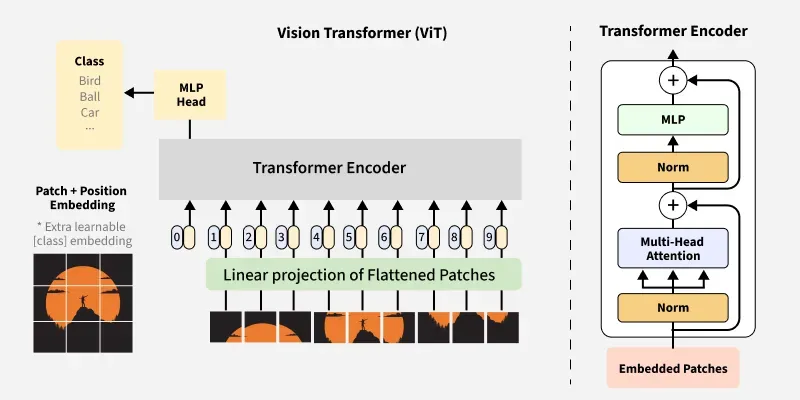
\includegraphics[width=0.9\linewidth]{images/vit.png}
    \caption[معماری مبدل بینایی]{معماری مبدل بینایی (\lr{ViT}) شامل تقسیم تصویر به تکه‌ها، تعبیه خطی و رمزگذار مبدل.}
    \label{fig:ch1-vit-arch}
\end{figure}

\section{تنظیم دقیق پارامتر-کارا (\lr{PEFT})}
\label{sec:ch1-peft}
با رشد نمایی ابعاد مدل‌های زبانی و تصویری، تنظیم دقیق کامل\LTRfootnote{Full Fine-Tuning} تمام پارامترها برای هر کاربرد جدید بسیار پرهزینه و گاهی غیرممکن شده است. روش‌های تنظیم دقیق پارامتر-کارا\LTRfootnote{Parameter-Efficient Fine-Tuning} راهکاری برای این چالش هستند. هدف \lr{PEFT} دستیابی به عملکردی مشابه تنظیم دقیق کامل، اما با تغییر تعداد بسیار اندکی از پارامترهاست. در ادامه دو مورد از مهم‌ترین این روش‌ها، یعنی تنظیم پیشوند و تنظیم جانبی تشریح می‌شوند.

\subsection{تنظیم پیشوند (\lr{Prefix Tuning})}
روش تنظیم پیشوند، الهام‌گرفته از مهندسی پرامپت است اما به جای استفاده از توکن‌های گسسته، از بردارهای پیوسته قابل یادگیری استفاده می‌کند. در این روش، یک دنباله از بردارهای پیوسته\LTRfootnote{Continuous Vectors} به نام «پیشوند» ($P$) به ابتدای ورودی مدل اضافه می‌شود. اگر $x$ ورودی و $y$ خروجی باشد، مدل زبانی با پارامترهای $\phi$ احتمال شرطی $p_\phi(y|x)$ را مدل‌سازی می‌کند. در تنظیم پیشوند، پارامترهای اصلی مدل $\phi$ ثابت نگه‌داشته می‌شوند و تنها پارامترهای پیشوند $\theta_P$ آموزش می‌بینند. برای یک توکن در گام $i$، وضعیت پنهان $h_i$ به صورت زیر محاسبه می‌شود:
\begin{equation}
    h_i = \begin{cases}
    P[i], & \text{if } i < \text{len}(P) \\
    \text{LM}(z_i, h_{<i}, \phi), & \text{otherwise}
    \end{cases}
\end{equation}
که در آن $P$ ماتریس پارامترهای پیشوند است. این مکانیزم به مدل اجازه می‌دهد تا بدون تغییر وزن‌های اصلی، با زمینه\LTRfootnote{Context} جدیدی که توسط پیشوند ایجاد شده، خود را با وظیفه جدید وفق دهد.

\subsection{تنظیم جانبی (\lr{Side-Tuning})}
روش تنظیم جانبی یکی دیگر از رویکردهای کارآمد است که در آن به جای تغییر وزن‌های اصلی مدل، یک شاخه جانبی کوچک و سبک به موازات مدل اصلی اضافه می‌شود. در این روش، مدل اصلی (که معمولاً بسیار بزرگ است) به صورت منجمد باقی می‌ماند و تنها پارامترهای شاخه جانبی آموزش می‌بینند. خروجی‌های این شاخه با خروجی‌های مدل اصلی ادغام می‌شوند تا رفتار مدل برای وظیفه جدید تطبیق یابد. این روش مزیت مهمی دارد، زیرا دانش پیش‌آموزش‌دیده مدل اصلی را تا حد زیادی حفظ می‌کند و از پدیده «فراموشی فاجعه‌بار» جلوگیری می‌کند. همچنین به دلیل سبک بودن شاخه جانبی، هزینه محاسباتی آموزش کاهش می‌یابد \cite{8409325,5294562}.

\section{مجموعه‌داده ImageNet}
\label{sec:ch1-imagenet}
مجموعه‌داده \lr{ImageNet} یکی از بزرگ‌ترین و تأثیرگذارترین منابع داده در تاریخ بینایی ماشین است که نقشی محوری در پیشرفت‌های اخیر یادگیری عمیق ایفا کرده است \cite{5206848}. این پروژه با هدف فراهم کردن یک پایگاه داده تصویری جامع و سازمان‌یافته بر اساس سلسله‌مراتب معنایی \lr{WordNet} راه‌اندازی شد. در این ساختار، مفاهیم به صورت دسته‌هایی از کلمات هم‌معنی\LTRfootnote{Synsets} گروه‌بندی شده‌اند و برای هر مفهوم، صدها یا هزاران تصویر جمع‌آوری و توسط انسان برچسب‌گذاری شده است. اهمیت این مجموعه‌داده فراتر از حجم آن است؛ تنوع قابل توجه تصاویر از زوایای دید متفاوت، شرایط نوری گوناگون و انسدادهای جزئی باعث شده تا مدل‌هایی که روی آن آموزش می‌بینند، بازنمایی‌های بصری بسیار غنی و قابل تعمیمی را یاد بگیرند که در بسیاری از وظایف پایین‌دستی\LTRfootnote{Downstream Tasks} کاربرد دارد.

از نظر خصوصیات آماری، نسخه کامل \lr{ImageNet} شامل بیش از ۱۴ میلیون تصویر برچسب‌خورده است که بیش از ۲۱ هزار دسته هم‌معنی مختلف را پوشش می‌دهند. با این حال، نسخه‌ای که بیشتر در تحقیقات و رقابت‌های علمی مورد ارجاع قرار می‌گیرد، زیرمجموعه‌ای است که برای چالش بازشناسی بصری در مقیاس بزرگ\LTRfootnote{ILSVRC} استفاده شده و به \lr{ImageNet-1K} مشهور است. این نسخه شامل حدود \lr{1.28} میلیون تصویر آموزشی و ۵۰ هزار تصویر اعتبارسنجی در ۱۰۰۰ کلاس متنوع است که اشیاء روزمره، حیوانات، وسایل نقلیه و مناظر طبیعی را در بر می‌گیرد. علاوه بر این، نسخه بزرگ‌تر \lr{ImageNet-21K} که شامل تمام دسته‌ها است، امروزه به طور فزاینده‌ای برای پیش‌آموزش مدل‌های عظیم مانند \lr{Vision Transformers} استفاده می‌شود، زیرا حجم داده‌های بیشتر در آن به بهبود کارایی مدل در مقیاس‌های بزرگ کمک می‌کند. خلاصه‌ای از مشخصات آماری نسخه \lr{ImageNet-1K} در جدول \ref{tab:ch1-imagenet-stats} ارائه شده است.

\begin{table}[ht]
    \centering
    \caption[اطلاعات آماری \lr{ImageNet}]{اطلاعات آماری مجموعه‌داده \lr{ImageNet}}
    \label{tab:ch1-imagenet-stats}
    \begin{tabular}{|r|c|}
        \hline
        \textbf{ویژگی} & \textbf{مقدار} \\
        \hline
        تعداد کلاس‌ها (\lr{ImageNet-1K}) & ۱۰۰۰ \\
        \hline
        تصاویر آموزشی & ۱,۲۸۱,۱۶۷ \\
        \hline
        تصاویر اعتبارسنجی & ۵۰,۰۰۰ \\
        \hline
        تصاویر آزمون & ۱۰۰,۰۰۰ \\
        \hline
        سال انتشار & ۲۰۰۹ \\
        \hline
    \end{tabular}
\end{table}

\section{معیارهای ارزیابی}
\label{sec:ch1-evaluation-metrics}
برای مقایسه کمی مدل‌ها از سه معیار استاندارد استفاده شده است: \lr{FID} برای فاصله توزیعی، \lr{KID} برای برآورد مبتنی بر \lr{MMD} و \lr{LPIPS-Mean} برای شباهت ادراکی مبتنی بر ویژگی‌های عمیق \cite{heusel2017fid,binkowski2018kid,zhang2018lpips}. در ارزیابی اصلی، \lr{FID} با پروتکل \lr{FID-50K} روی ۵۰٬۰۰۰ نمونه تولیدشده از همه کلاس‌های \lr{ImageNet-1K} گزارش می‌شود. معیار \lr{KID} نیز مکمل \lr{FID} است، زیرا به‌صورت برآورد بدون سوگیری فاصله توزیعی عمل می‌کند. برای سنجش کیفیت ادراکی، \lr{LPIPS-Mean} میانگین فاصله ادراکی همه زوج‌های تصویر تولیدی و واقعی متناظر در هر کلاس را اندازه می‌گیرد و سپس روی کلاس‌ها میانگین گیری می‌شود \cite{5206848,2212.09748}.

معیار نخست، فاصله فریشه اینسپشن\LTRfootnote{Fréchet Inception Distance} (\lr{FID}) است. در این معیار، تصاویر واقعی و تولیدشده ابتدا با شبکه \lr{Inception} به فضای ویژگی نگاشت می‌شوند و سپس هر توزیع ویژگی با یک توزیع گاوسی تقریب زده می‌شود. اگر میانگین و کوواریانس ویژگی‌های تصاویر واقعی به‌ترتیب $\mu_r$ و $\Sigma_r$، و میانگین و کوواریانس ویژگی‌های تصاویر تولیدشده $\mu_g$ و $\Sigma_g$ باشد، مقدار \lr{FID} به صورت زیر محاسبه می‌شود \cite{heusel2017fid}:
\begin{equation}
    \label{eq:fid}
    \mathrm{FID} =
    \|\mu_r - \mu_g\|_2^2 +
    \operatorname{Tr}\left(\Sigma_r + \Sigma_g - 2(\Sigma_r \Sigma_g)^{\frac{1}{2}}\right).
\end{equation}
در رابطه \ref{eq:fid}، عبارت اول فاصله میانگین‌های دو توزیع و عبارت دوم تفاوت ساختار کوواریانس آن‌ها را اندازه‌گیری می‌کند. مقدار کمتر \lr{FID} نشان می‌دهد توزیع ویژگی‌های تصاویر تولیدشده به توزیع تصاویر واقعی نزدیک‌تر است \cite{heusel2017fid}.

معیار دوم، فاصله هسته‌ای اینسپشن\LTRfootnote{Kernel Inception Distance} (\lr{KID}) است که بر پایه بیشینه میانگین اختلاف\LTRfootnote{Maximum Mean Discrepancy - MMD} تعریف می‌گردد. اگر $X=\{x_i\}_{i=1}^{m}$ ویژگی‌های تصاویر واقعی و $Y=\{y_j\}_{j=1}^{n}$ ویژگی‌های تصاویر تولیدشده باشند، برآورد بدون سوگیری \lr{MMD} به صورت زیر نوشته می‌شود \cite{binkowski2018kid}:
\begin{equation}
    \label{eq:kid}
    \mathrm{KID} =
    \frac{1}{m(m-1)}\sum_{i \ne j} k(x_i,x_j)
    + \frac{1}{n(n-1)}\sum_{i \ne j} k(y_i,y_j)
    - \frac{2}{mn}\sum_{i=1}^{m}\sum_{j=1}^{n} k(x_i,y_j).
\end{equation}
در این رابطه، $k(\cdot,\cdot)$ معمولاً یک هسته چندجمله‌ای روی ویژگی‌های اینسپشن است، مانند $k(x,y) = (\frac{1}{d}x^\top y + 1)^3$ که در آن $d$ بعد بردار ویژگی است. مقدار کمتر \lr{KID} نشان‌دهنده شباهت بیشتر دو مجموعه تصویر است و به دلیل برآورد بدون سوگیری، در مجموعه‌های نمونه کوچک نیز قابل استفاده است \cite{binkowski2018kid}.

معیار سوم، شباهت ادراکی یادگرفته‌شده قطعه‌های تصویر\LTRfootnote{Learned Perceptual Image Patch Similarity} (\lr{LPIPS}) است که شباهت ادراکی دو تصویر را با استفاده از فاصله ویژگی‌های میانی یک شبکه عمیق محاسبه می‌کند. اگر $\hat{y}^{\,l}_{hw}$ و $\hat{y}^{\,\prime l}_{hw}$ ویژگی‌های نرمال‌شده دو تصویر در لایه $l$ و مکان مکانی $(h,w)$ باشند، مقدار \lr{LPIPS} به صورت زیر تعریف می‌شود \cite{zhang2018lpips}:
\begin{equation}
    \label{eq:lpips}
    \mathrm{LPIPS}(x,x') =
    \sum_l \frac{1}{H_l W_l}
    \sum_{h=1}^{H_l}\sum_{w=1}^{W_l}
    \left\| w_l \odot \left(\hat{y}^{\,l}_{hw} - \hat{y}^{\,\prime l}_{hw}\right) \right\|_2^2.
\end{equation}
در رابطه \ref{eq:lpips}، $w_l$ وزن‌های یادگرفته‌شده برای اهمیت کانال‌های لایه $l$، و $H_l$ و $W_l$ ابعاد مکانی نقشه ویژگی هستند. برخلاف \lr{FID} و \lr{KID} که توزیع کلی مجموعه تصاویر را مقایسه می‌کنند، \lr{LPIPS} روی شباهت ادراکی زوج‌تصویرها تمرکز دارد و به جزئیات محلی، بافت و ساختارهای بصری حساس‌تر است؛ بنابراین مقدار کمتر آن نشان‌دهنده شباهت ادراکی بیشتر است \cite{zhang2018lpips}.

در این پایان‌نامه، نسخه گزارش‌شده از این معیار با عنوان \lr{LPIPS-Mean} تعریف می‌شود. اگر $G_c$ مجموعه تصاویر تولیدشده برای کلاس $c$ و $R_c$ مجموعه تصاویر واقعی همان کلاس باشد، مقدار کلاسی این معیار به صورت زیر محاسبه می‌شود:
\begin{equation}
    \label{eq:lpips-mean}
    \mathrm{LPIPS\text{-}Mean}_c =
    \frac{1}{|G_c||R_c|}
    \sum_{g \in G_c}\sum_{r \in R_c}
    d_{\mathrm{LPIPS}}(g,r).
\end{equation}
در نهایت، میانگین \lr{LPIPS-Mean} روی کلاس‌های ارزیابی‌شده گزارش می‌شود. این تعریف با مقایسه همه زوج‌های تولیدی و واقعی، دید دقیق‌تری از فاصله ادراکی میان خروجی مدل و داده واقعی فراهم می‌کند.

\chapter{پیشینه پژوهش}\label{chp2}

در فصل پیش، مفاهیم پایه‌ای مدل‌های مولد، مدل‌های انتشار و مبدل‌های بینایی در سطح مقدماتی معرفی شد. در این فصل، تمرکز از تعریف اولیه به سمت چارچوب‌های پژوهشی و مسیر تکامل مدل‌های انتشار می‌رود؛ به‌گونه‌ای که ابتدا فرمول‌بندی‌های اصلی این خانواده از مدل‌ها، شامل \lr{DDPM}، مدل‌های مبتنی بر امتیاز، فرمول‌بندی پیوسته و روش‌های نمونه‌برداری مرور می‌شوند. سپس نشان داده می‌شود که چرا پس از تثبیت این چارچوب‌ها، انتخاب معماری شبکه حذف نویز اهمیت پیدا کرده و چگونه این مسیر به مدل‌های انتشار مبتنی بر مبدل، به‌ویژه \lr{DiT}، منتهی شده است. در ادامه، روندهای تکمیلی از نظر مقیاس‌پذیری، کنترل‌پذیری و حفظ جزئیات محلی بررسی می‌گردد. سپس معماری‌های جریان دوگانه و روش‌های تجمیع ویژگی مطالعه می‌شوند تا مبنای نظری شاخه وضوح‌بالای پیشنهادی روشن شود. در پایان نیز روش‌های تنظیم دقیق، به‌ویژه رویکردهای پارامتر-کارا، بررسی می‌شوند؛ زیرا معماری پیشنهادی این پژوهش بر ترکیب یک بدنه اصلی منجمد با یک شاخه جانبی آموزش‌پذیر استوار است \cite{0214306,2212.09748,chen2021crossvit,8409325}.

\section{چارچوب‌های اصلی مدل‌های انتشار}
\label{sec:ch2-diffusion-frameworks}
توضیح مقدماتی فصل پیش نشان داد که مدل انتشار از دو مسیر نویزدهی و حذف نویز تشکیل می‌شود. در پیشینه پژوهش، این ایده در چند فرمول‌بندی اصلی توسعه یافته است که هر یک زاویه متفاوتی از همان مسئله را برجسته می‌کنند: در \lr{DDPM}\LTRfootnote{Denoising Diffusion Probabilistic Models}، فرایند تولید به‌صورت یک زنجیره مارکوف گسسته مدل می‌شود؛ در مدل‌های مبتنی بر امتیاز، هدف یادگیری گرادیان لگاریتم چگالی داده‌های نویزی است؛ و در فرمول‌بندی پیوسته، هر دو نگاه در قالب معادلات دیفرانسیل تصادفی و معادلات دیفرانسیل معمولی قابل بیان می‌شوند \cite{sohlDickstein2015deepUnsupervised,ho2020ddpm,song2019scoreGenerative,song2021scoreSDE}. این بخش برای جلوگیری از تکرار فصل اول، بر تفاوت این چارچوب‌ها، روابط ریاضی کلیدی و جایگاه آن‌ها در تعریف نقش شبکه حذف نویز تمرکز دارد.

\subsection{مدل‌های \lr{DDPM}}
در فرمول‌بندی احتمالاتی، داده واقعی با $x_0 \sim q_{\text{data}}(x)$ نمایش داده می‌شود و یک زمان‌بندی نویز\LTRfootnote{Noise Schedule} شامل ضرایب $\{\beta_t\}_{t=1}^{T}$ مشخص می‌کند که در هر گام چه مقدار نویز گاوسی به داده افزوده شود. اگر $\alpha_t = 1-\beta_t$ و $\bar{\alpha}_t = \prod_{s=1}^{t}\alpha_s$ باشد، فرایند رو به جلو به صورت زیر نوشته می‌شود \cite{sohlDickstein2015deepUnsupervised,ho2020ddpm}:
\begin{equation}
q(x_t|x_{t-1}) = \mathcal{N}\left(x_t; \sqrt{\alpha_t}x_{t-1}, (1-\alpha_t)I\right).
\end{equation}
مزیت این تعریف آن است که نمونه نویزی در هر گام را می‌توان مستقیماً از $x_0$ نیز به دست آورد:
\begin{equation}
q(x_t|x_0) = \mathcal{N}\left(x_t; \sqrt{\bar{\alpha}_t}x_0, (1-\bar{\alpha}_t)I\right),
\end{equation}
یا به شکل بازپارامتری‌شده:
\begin{equation}
x_t = \sqrt{\bar{\alpha}_t}x_0 + \sqrt{1-\bar{\alpha}_t}\epsilon,\quad \epsilon \sim \mathcal{N}(0,I).
\end{equation}
بنابراین، آموزش مدل به معنای یادگیری مسیر معکوس از $x_t$ به $x_{t-1}$ است:
\begin{equation}
p_\theta(x_{t-1}|x_t) = \mathcal{N}\left(x_{t-1}; \mu_\theta(x_t,t), \Sigma_\theta(x_t,t)\right).
\end{equation}
در \lr{DDPM}، به‌جای پیش‌بینی مستقیم $x_{t-1}$، شبکه معمولاً نویز افزوده‌شده را تخمین می‌زند. این انتخاب باعث می‌شود تابع هدف عملی به یک خطای میانگین مربعات ساده تبدیل شود \cite{ho2020ddpm}:
\begin{equation}
\mathcal{L}_{\text{\lr{DDPM}}} =
\mathbb{E}_{x_0,\epsilon,t}
\left[
\left\|
\epsilon - \epsilon_\theta(x_t,t,c)
\right\|_2^2
\right],
\end{equation}
که در آن $c$ می‌تواند شرطی مانند برچسب کلاس یا متن باشد. همین رابطه در مدل‌های مبتنی بر \lr{DiT} نیز حفظ می‌شود؛ تفاوت اصلی در آن است که تابع $\epsilon_\theta$ به‌جای یک شبکه پیچشی، با یک معماری مبدلی پیاده‌سازی می‌شود \cite{2212.09748}.

\subsection{مدل‌های مبتنی بر امتیاز}
دیدگاه مبتنی بر امتیاز\LTRfootnote{Score-Based Modeling} مسئله را از زاویه دیگری بیان می‌کند. در این رویکرد، مدل به‌جای تخمین مستقیم چگالی داده، تابع امتیاز توزیع داده‌های نویزی را یاد می‌گیرد \cite{song2019scoreGenerative,song2021scoreSDE}:
\begin{equation}
s_\theta(x_t,t) \approx \nabla_{x_t}\log q_t(x_t).
\end{equation}
تابع امتیاز جهت افزایش احتمال داده را در فضای نمونه نشان می‌دهد؛ به بیان دیگر، مشخص می‌کند یک نمونه نویزی باید در چه جهتی حرکت کند تا به نواحی محتمل‌تر توزیع داده نزدیک شود. ارتباط این دیدگاه با \lr{DDPM} از رابطه نویز گاوسی روشن می‌شود. اگر $\sigma_t^2 = 1-\bar{\alpha}_t$ باشد، امتیاز توزیع شرطی نویزی با نویز افزوده‌شده نسبت مستقیم دارد:
\begin{equation}
\nabla_{x_t}\log q(x_t|x_0) = -\frac{\epsilon}{\sigma_t}.
\end{equation}
بنابراین، پیش‌بینی نویز در \lr{DDPM} و تخمین امتیاز در مدل‌های مبتنی بر امتیاز دو بیان نزدیک از یک مسئله هستند. این ارتباط اهمیت زیادی دارد، زیرا نشان می‌دهد روش‌های مختلف مدل‌های انتشار تنها نام‌گذاری‌های جداگانه نیستند، بلکه از نظر ریاضی به یک خانواده مشترک تعلق دارند \cite{song2021scoreSDE,0214306}.

\subsection{مدل‌های انتشار مبتنی بر \lr{SDE}}
برای یکپارچه‌سازی دیدگاه‌های گسسته و مبتنی بر امتیاز، مدل‌های انتشار را می‌توان در زمان پیوسته با معادله دیفرانسیل تصادفی\LTRfootnote{Stochastic Differential Equation} بیان کرد \cite{song2021scoreSDE}:
\begin{equation}
d x = f(x,t)\,dt + g(t)\,d w,
\end{equation}
که در آن $f(x,t)$ جمله رانش، $g(t)$ شدت نویز و $w$ فرایند وینر است. در مسیر رو به جلو، این معادله داده را به‌تدریج به توزیع ساده‌ای مانند نرمال استاندارد نزدیک می‌کند. مسیر معکوس نیز با استفاده از تابع امتیاز قابل نوشتن است:
\begin{equation}
d x =
\left[
f(x,t) - g(t)^2\nabla_x\log p_t(x)
\right]dt
+ g(t)\,d\bar{w}.
\end{equation}
این رابطه نشان می‌دهد که اگر مدل بتواند امتیاز $\nabla_x\log p_t(x)$ را تخمین بزند، می‌توان مسیر تولید را از نویز به داده طی کرد. همچنین یک معادله دیفرانسیل معمولی\LTRfootnote{Ordinary Differential Equation} متناظر، موسوم به \lr{Probability Flow ODE}، وجود دارد:
\begin{equation}
\frac{d x}{dt} =
f(x,t) - \frac{1}{2}g(t)^2\nabla_x\log p_t(x).
\end{equation}
این نگاه پیوسته برای طراحی نمونه‌بردارهای سریع‌تر و تحلیل ارتباط میان خانواده‌های مختلف مدل‌های انتشار اهمیت دارد؛ زیرا انتخاب زمان‌بندی نویز، گام‌های حل عددی و پارامترسازی شبکه را از یکدیگر تفکیک می‌کند \cite{song2021scoreSDE,karras2022edm}.

\subsection{نمونه‌برداری، \lr{DDIM} و هدایت تولید}
یکی از محدودیت‌های اولیه مدل‌های انتشار، نیاز به تعداد زیاد گام‌های نمونه‌برداری بود. \lr{DDIM}\LTRfootnote{Denoising Diffusion Implicit Models} نشان داد که می‌توان با تعریف یک مسیر غیرمارکوفی، نمونه‌برداری را با گام‌های کمتر انجام داد، در حالی که از همان شبکه آموزش‌دیده استفاده می‌شود \cite{song2021ddim}. ابتدا تخمین تصویر پاک از روی نمونه نویزی محاسبه می‌شود:
\begin{equation}
\hat{x}_0 =
\frac{x_t - \sqrt{1-\bar{\alpha}_t}\epsilon_\theta(x_t,t,c)}
{\sqrt{\bar{\alpha}_t}}.
\end{equation}
سپس نمونه گام قبلی با ترکیب $\hat{x}_0$ و نویز پیش‌بینی‌شده ساخته می‌شود. در حالت کلی:
\begin{equation}
x_{t-1} =
\sqrt{\bar{\alpha}_{t-1}}\hat{x}_0
+ \sqrt{1-\bar{\alpha}_{t-1}-\sigma_t^2}\epsilon_\theta(x_t,t,c)
+ \sigma_t z,
\end{equation}
که در آن $z \sim \mathcal{N}(0,I)$ است. با انتخاب $\sigma_t=0$، فرایند نمونه‌برداری قطعی می‌شود و می‌تواند با تعداد گام کمتر اجرا گردد. در مدل‌های شرطی، علاوه بر سرعت نمونه‌برداری، کنترل خروجی نیز اهمیت دارد. یکی از روش‌های رایج برای افزایش کنترل‌پذیری، هدایت تولید است؛ به این معنا که مسیر حذف نویز فقط از توزیع کلی داده پیروی نکند، بلکه به سمت شرط مورد نظر، مانند برچسب کلاس، سوق داده شود. روش‌های اولیه هدایت معمولاً به یک طبقه‌بند جداگانه نیاز داشتند تا در هر گام نمونه‌برداری گرادیان احتمال کلاس را محاسبه کند. در مقابل، راهنمایی بدون طبقه‌بند\LTRfootnote{Classifier-Free Guidance} یا \lr{CFG} این وابستگی را حذف می‌کند و همان شبکه حذف نویز را هم برای پیش‌بینی شرطی و هم برای پیش‌بینی بی‌شرط به کار می‌گیرد \cite{ho2022classifierFreeGuidance}.

برای ممکن شدن این کار، در زمان آموزش، شرط $c$ با احتمالی مشخص حذف و با شرط تهی $\emptyset$ جایگزین می‌شود. بنابراین مدل واحد $\epsilon_\theta$ یاد می‌گیرد هم نویز را در حالت شرطی، یعنی $\epsilon_\theta(x_t,t,c)$، و هم در حالت بی‌شرط، یعنی $\epsilon_\theta(x_t,t,\emptyset)$، تخمین بزند. در زمان نمونه‌برداری، این دو پیش‌بینی با یکدیگر ترکیب می‌شوند:
\begin{equation}
\epsilon_{\text{\lr{cfg}}} =
\epsilon_\theta(x_t,t,\emptyset)
+ w\left(
\epsilon_\theta(x_t,t,c) -
\epsilon_\theta(x_t,t,\emptyset)
\right),
\end{equation}
که در آن $w$ شدت هدایت را کنترل می‌کند. اختلاف
$\epsilon_\theta(x_t,t,c)-\epsilon_\theta(x_t,t,\emptyset)$
را می‌توان جهت اثر شرط دانست؛ یعنی بخشی از پیش‌بینی نویز که به حضور شرط وابسته است. وقتی $w=0$ باشد، نمونه‌برداری عملاً بی‌شرط است. وقتی $w=1$ باشد، خروجی معادل پیش‌بینی شرطی معمولی می‌شود. برای مقادیر بزرگ‌تر از یک، نمونه‌بردار در جهت شرط فراتر از پیش‌بینی شرطی حرکت می‌کند و در نتیجه تصویر معمولاً نشانه‌های معنایی مرتبط با کلاس را واضح‌تر نشان می‌دهد.

تأثیر \lr{CFG} دوگانه است. از یک سو، افزایش $w$ می‌تواند وفاداری شرطی\LTRfootnote{Conditional Fidelity} را بهبود دهد؛ برای مثال، در تولید کلاسی \lr{ImageNet} احتمال اینکه نمونه تولیدشده واقعاً با کلاس خواسته‌شده سازگار باشد بیشتر می‌شود. از سوی دیگر، اگر ضریب هدایت بیش از حد بزرگ شود، مدل به ناحیه محدودتری از توزیع داده رانده می‌شود. این موضوع می‌تواند تنوع نمونه‌ها را کاهش دهد، بافت‌ها را بیش از حد تیز یا اشباع کند، و حتی معیارهای توزیعی مانند \lr{FID} و \lr{KID} را بدتر کند. بنابراین \lr{CFG} یک اهرم تنظیم بین وفاداری به شرط و تنوع توزیعی است، نه یک بهبود بدون هزینه. از نظر محاسباتی نیز نمونه‌برداری با \lr{CFG} معمولاً به دو پیش‌بینی شرطی و بی‌شرط در هر گام نیاز دارد و هزینه استنتاج شبکه حذف نویز را افزایش می‌دهد، هرچند به آموزش یا نگهداری طبقه‌بند جداگانه احتیاج ندارد \cite{ho2022classifierFreeGuidance}.

این رابطه برای این پایان‌نامه مهم است، زیرا ارزیابی اصلی روی تولید شرطی \lr{ImageNet-1K} انجام می‌شود و لازم است نمونه‌ها علاوه بر کیفیت بصری، به برچسب کلاس انتخاب‌شده نیز وفادار باشند. در فصل آزمایش‌ها، مقدار \lr{CFG} به‌عنوان یک ابرپارامتر نمونه‌برداری گزارش و تحلیل می‌شود تا اثر آن از اثر تغییرات معماری \lr{DuoDiT} جدا بماند.

\begin{table}[htbp]
    \centering
    \caption[مقایسه چارچوب‌های اصلی مدل‌های انتشار]{مقایسه چارچوب‌های اصلی مدل‌های انتشار}
    \label{tab:ch2-diffusion-frameworks}
    \resizebox{\textwidth}{!}{%
    \begin{tabular}{p{0.22\textwidth}p{0.38\textwidth}p{0.32\textwidth}}
        \hline
        \textbf{چارچوب} & \textbf{ایده اصلی} & \textbf{رابطه یا هدف کلیدی} \\
        \hline
        \lr{DDPM} & مدل‌سازی گسسته مسیر نویزدهی و حذف نویز & پیش‌بینی $\epsilon_\theta(x_t,t,c)$ با خطای میانگین مربعات \\
        مدل‌های مبتنی بر امتیاز & یادگیری گرادیان لگاریتم چگالی داده‌های نویزی & $s_\theta(x_t,t) \approx \nabla_{x_t}\log q_t(x_t)$ \\
        \lr{SDE/ODE} & بیان پیوسته فرایند نویزدهی و تولید & $dx=f(x,t)dt+g(t)dw$ \\
        \lr{DDIM} و نمونه‌بردارها & کاهش تعداد گام‌های تولید با مسیرهای جایگزین & بازسازی $\hat{x}_0$ از روی $x_t$ و $\epsilon_\theta$ \\
        \lr{CFG} & افزایش وفاداری شرطی در نمونه‌برداری بدون طبقه‌بند جداگانه & ترکیب $\epsilon_\theta(x_t,t,c)$ و $\epsilon_\theta(x_t,t,\emptyset)$ با ضریب $w$ \\
        \hline
    \end{tabular}%
    }
\end{table}

\section{مدل‌های انتشار مبتنی بر مبدل}
پس از تثبیت چارچوب‌های احتمالاتی، مبتنی بر امتیاز و پیوسته در مدل‌های انتشار، تمرکز پژوهش‌ها از تعریف فرایند حذف نویز به سمت طراحی معماری شبکه حذف نویز تغییر کرد؛ زیرا کیفیت تولید فقط به تابع هدف انتشار وابسته نیست و عواملی مانند فضای نمایش، زمان‌بندی نویز، نوع شرط‌گذاری، نمونه‌بردار و ساختار شبکه نیز در عملکرد نهایی اثر دارند \cite{0214306,7811582,9851474}. در همین مسیر، موفقیت مبدل‌ها در پردازش توالی و سپس در بینایی ماشین باعث شد پژوهشگران از معماری‌های مبتنی بر توجه برای مدل‌های مولد تصویری استفاده کنند \cite{Vaswani2017,Dosovitskiy2020}. برخلاف \lr{U-Net}ها و شبکه‌های پیچشی که سوگیری محلی قوی دارند، مبدل‌ها با مدل‌سازی وابستگی‌های دوربرد میان توکن‌های تصویری می‌توانند ساختار سراسری تصویر را بهتر دنبال کنند؛ هرچند نبود سوگیری محلی ذاتی، هزینه توجه و نیاز به حفظ جزئیات مکانی همچنان چالش‌های مهمی هستند \cite{0017415,3153255,9511279}. بنابراین، مسئله اصلی این بخش آن است که چگونه می‌توان نقش تابع $\epsilon_\theta$ را از یک بدنه اصلی پیچشی به یک معماری مبدلی منتقل کرد و در عین حال شرط زمانی، شرط کلاسی و اطلاعات مکانی تصویر را به‌صورت پایدار حفظ نمود \cite{2212.09748,5638143,8106348}.

\subsection{مدل \lr{GenViT}}
مدل \lr{GenViT}\LTRfootnote{Generative ViT} یکی از تلاش‌های اولیه برای بررسی این ایده بود که آیا می‌توان بدنه اصلی مدل انتشار را با یک \lr{ViT} خالص پیاده‌سازی کرد یا نه \cite{2208.07791}. اهمیت این مدل در آن است که پیش از تثبیت خانواده \lr{DiT}، امکان استفاده از توکن‌های تصویری و اطلاعات گام زمانی در یک معماری تمام‌مبدلی را بررسی کرد.

در \lr{GenViT}، توکن‌های تصویر نویزی همراه با اطلاعات زمان پردازش می‌شوند و تابع زیان، یادگیری تولیدی و تمایزگر را در کنار یکدیگر قرار می‌دهد:
\begin{equation}
\mathcal{L}_{\text{\lr{total}}} = \mathcal{L}_{\text{\lr{diff}}} + \lambda \mathcal{L}_{\text{\lr{cls}}}
\end{equation}
که در آن $\mathcal{L}_{\text{diff}}$ خطای بازسازی نویز و $\mathcal{L}_{\text{cls}}$ خطای دسته‌بندی است. این مدل از نظر تاریخی نشان می‌دهد که مبدل‌ها فقط برای استخراج ویژگی تصویری به کار نمی‌روند، بلکه می‌توانند در خود مسیر تولید نیز نقش داشته باشند. نمای کلی این معماری در شکل \ref{fig:genvit} نمایش داده شده است \cite{2208.07791}.

\begin{figure}[H]
	\centering
	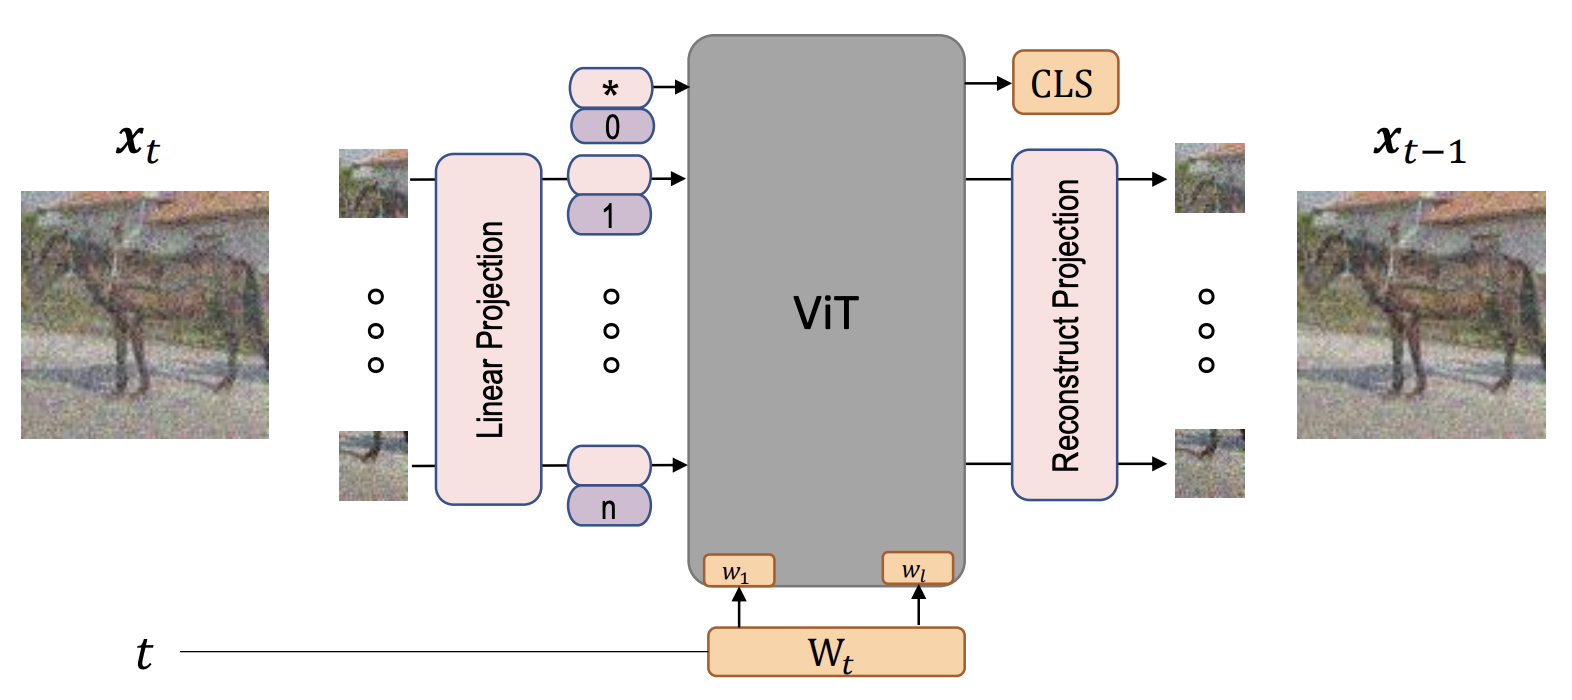
\includegraphics[width=0.9\textwidth]{images/gen_vit.png}
	\caption[معماری \lr{GenViT}]{معماری \lr{GenViT} که مبدل را در مدل انتشار ادغام می‌کند.}
	\label{fig:genvit}
\end{figure}

\subsection{مدل \lr{U-ViT}}
مدل \lr{U-ViT}\LTRfootnote{U-shaped Vision Transformer} مسئله دیگری را برجسته کرد: اگر شبکه حذف نویز کاملاً مبدلی باشد، چگونه می‌توان اطلاعات سطح پایین و جزئیات مکانی را در مسیر عمیق مدل حفظ کرد؟ بائو و همکاران با الهام از شکل \lr{U-Net}، اتصالات پرشی بلند\LTRfootnote{Long Skip Connections} را میان بلوک‌های کم‌عمق و عمیق مبدل وارد کردند تا اطلاعات محلی در طول فرایند حذف نویز از بین نرود \cite{2209.12152}.

در \lr{U-ViT}، تصویر نویزی، زمان و شرط‌هایی مانند برچسب کلاس همگی به صورت توکن پردازش می‌شوند و تخمین نویز $\epsilon_\theta(x_t, t, c)$ توسط یک شبکه تمام‌مبدلی انجام می‌گیرد. شکل \ref{fig:uvit} ساختار کلی این مدل را نشان می‌دهد. اهمیت \lr{U-ViT} برای این پایان‌نامه در آن است که نشان می‌دهد حتی در معماری‌های مبدلی نیز مسیرهای میان‌بر و چندسطحی برای حفظ جزئیات مکانی ضروری هستند \cite{2209.12152}.

\begin{figure}[H]
	\centering
	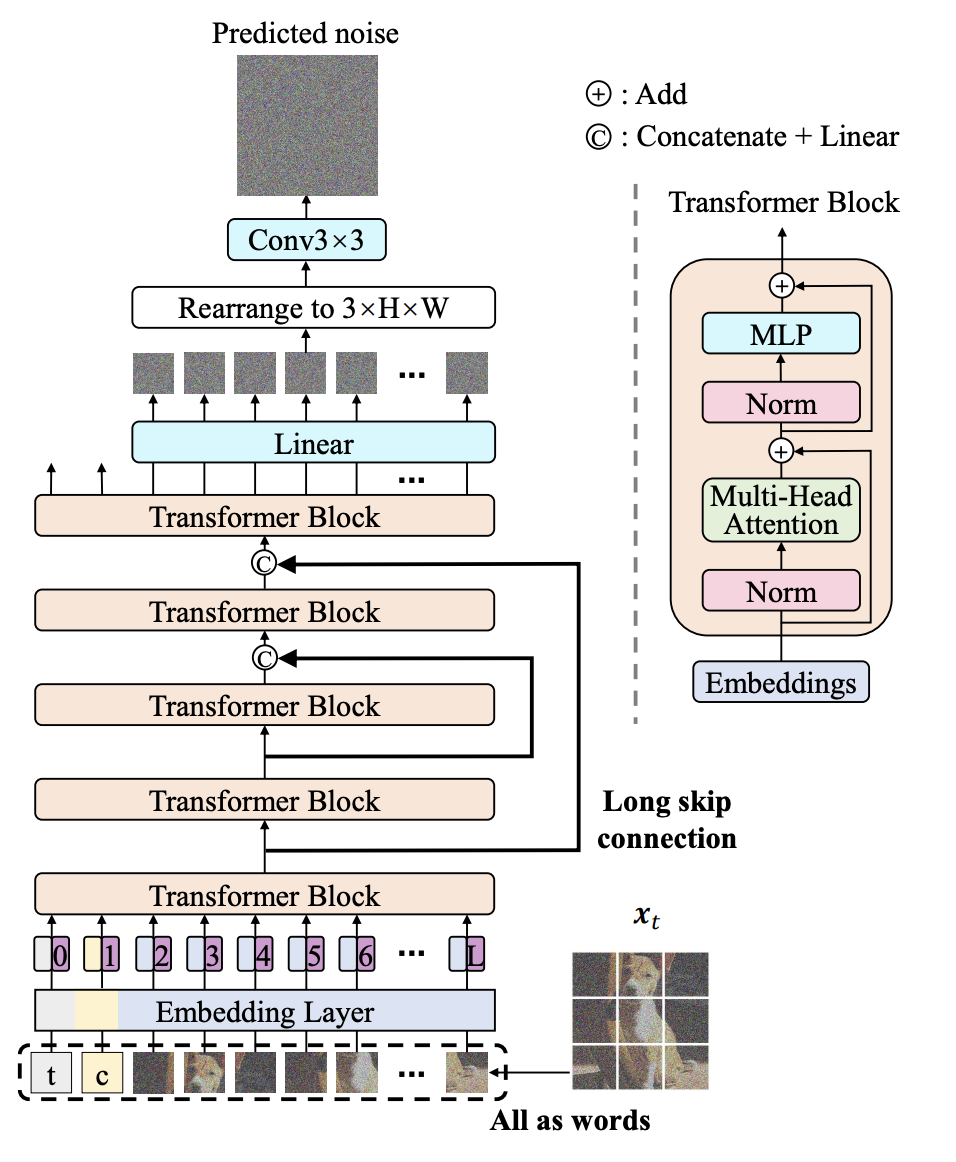
\includegraphics[width=0.9\textwidth]{images/u_vit.png}
	\caption[معماری \lr{U-ViT}]{معماری \lr{U-ViT} با اتصالات پرشی بلند بین بلوک‌های مبدل \cite{2209.12152}.}
	\label{fig:uvit}
\end{figure}

\subsection{مدل \lr{DiT}}
مدل مبدل انتشار\LTRfootnote{Diffusion Transformer} (\lr{DiT}) نقطه محوری این فصل است، زیرا نشان می‌دهد در مدل انتشار می‌توان معماری حذف نویز را از \lr{U-Net} به یک بدنه اصلی تمام‌مبدلی منتقل کرد، بدون آن‌که فرمول‌بندی انتشار تغییر کند \cite{2212.09748}. این مدل روی فضای نهان\LTRfootnote{Latent Space} عمل می‌کند؛ یعنی ابتدا تصویر به نمایش فشرده‌تری تبدیل می‌شود و سپس این نمایش به پچ‌ها و توکن‌ها شکسته می‌شود. پیبلز و شی نشان دادند که با افزایش تعداد پارامترها و حجم محاسبات، کیفیت تولید تصویر در این خانواده به‌صورت پیوسته بهبود می‌یابد.

معماری \lr{DiT} از بلوک‌های استاندارد \lr{ViT} استفاده می‌کند، اما برای تزریق اطلاعات زمان و کلاس از نرمال‌سازی لایه تطبیقی با مقداردهی صفر (\lr{adaLN-Zero}\LTRfootnote{Adaptive Layer Normalization with Zero Initialization}) بهره می‌برد. در این سازوکار، پارامترهای مقیاس ($\gamma$) و انتقال ($\beta$) در لایه‌های نرمال‌سازی از بردار زمان و کلاس پیش‌بینی می‌شوند:
\begin{equation}
\text{\lr{adaLN}}(h, t, c) = \gamma(t, c) \odot \text{\lr{Norm}}(h) + \beta(t, c)
\end{equation}
این روش، شرط‌گذاری را درون بلوک‌های مبدل وارد می‌کند و به مدل اجازه می‌دهد فرایند حذف نویز را در فضای فشرده‌تری نسبت به پیکسل‌ها انجام دهد. شکل \ref{fig:dit} ساختار کلی این معماری را نشان می‌دهد \cite{2212.09748}. از آنجا که معماری پیشنهادی این پایان‌نامه نیز یک شاخه مکمل را در کنار بدنه اصلی \lr{DiT} قرار می‌دهد، این مدل مرجع اصلی برای تحلیل‌های بعدی فصل است.

\begin{figure}[H]
	\centering
	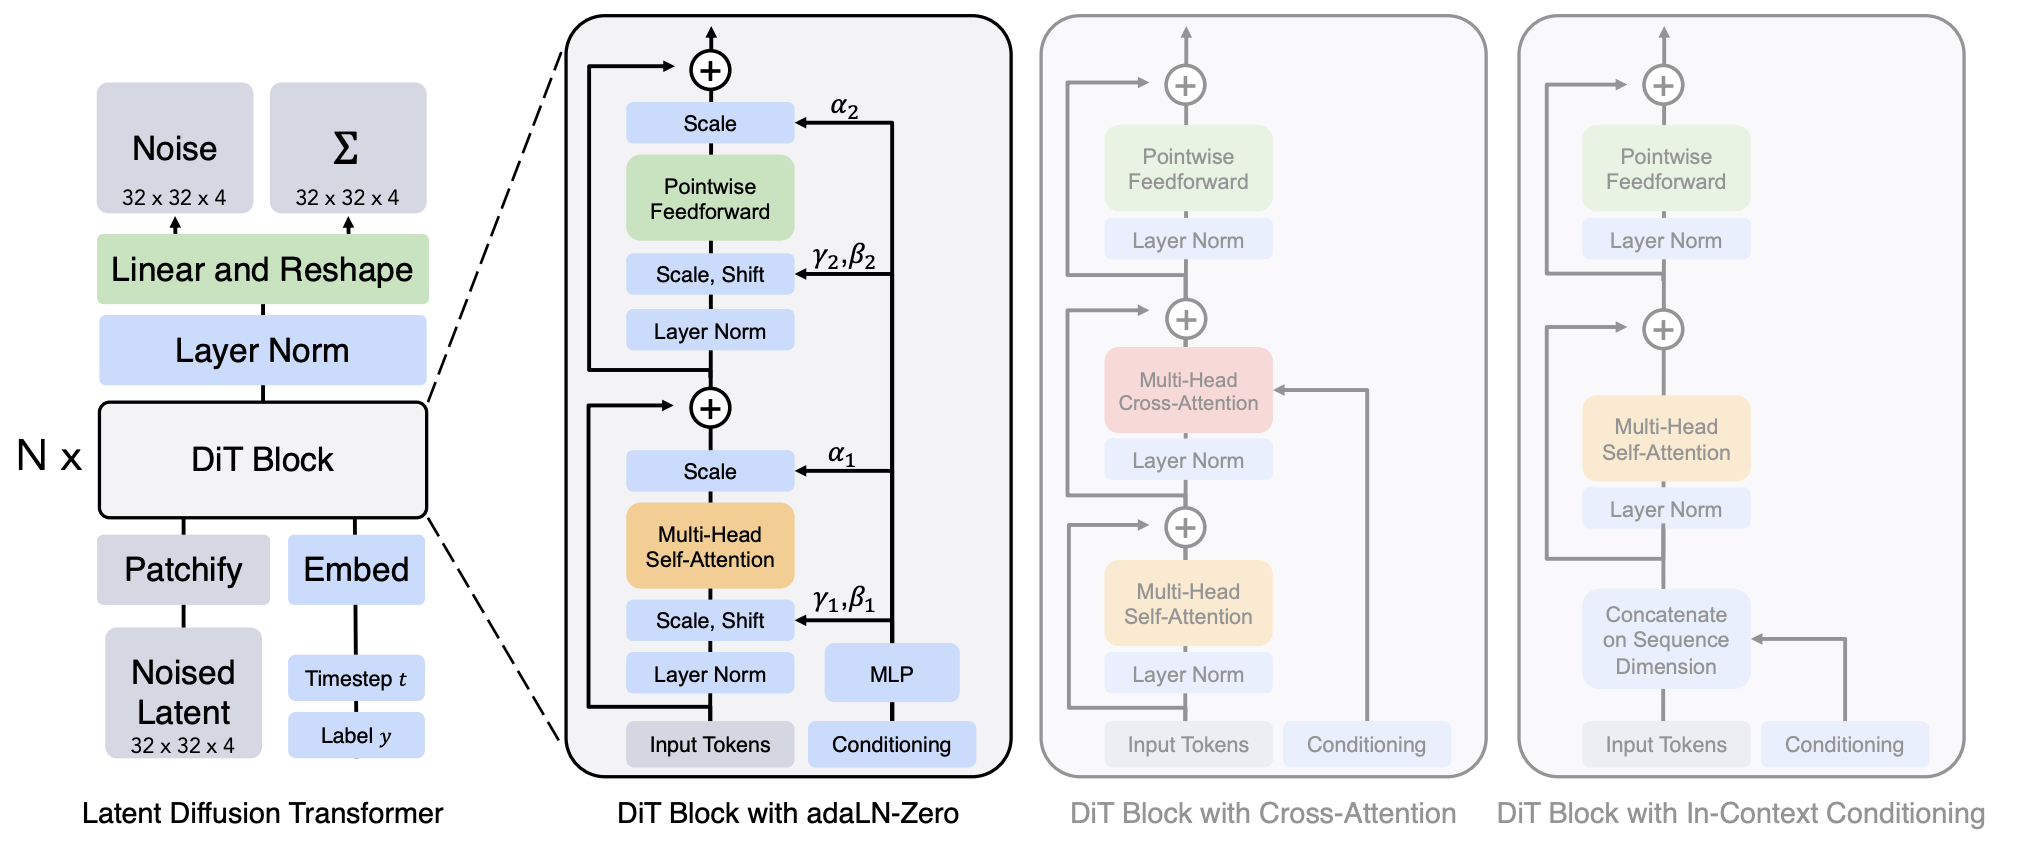
\includegraphics[width=0.9\textwidth]{images/base_dit.png}
	\caption[معماری \lr{DiT}]{معماری \lr{DiT} مبتنی بر بلوک‌های استاندارد مبدل و \lr{adaLN}.}
	\label{fig:dit}
\end{figure}

مدل \lr{DiffiT}\LTRfootnote{Diffusion Vision Transformer} بر محدودیت دیگری در مبدل‌های انتشار تمرکز دارد: نحوه وارد کردن زمان در فرایند توجه \cite{2312.02139v3}. در \lr{DiT}، زمان و کلاس عمدتاً از مسیر نرمال‌سازی تطبیقی وارد بلوک‌ها می‌شوند، اما \lr{DiffiT} یک مکانیزم خود توجه وابسته به زمان\LTRfootnote{Time-Dependent Self-Attention - TMSA} معرفی می‌کند تا ماتریس‌های توجه نیز مستقیماً از گام زمانی اثر بگیرند.

در این مدل، توکن زمان به‌صورت پویا در لایه‌های توجه حضور دارد و رابطه توجه ضرب داخلی مقیاس‌شده، که در رابطه \ref{eq:scaled-dot-product-attention} معرفی شد، با پرسش، کلید و مقدار وابسته به زمان نوشته می‌شود:
\begin{equation}
\text{\lr{Attention}}(Q_t, K_t, V_t) = \text{\lr{softmax}}\left(\frac{Q_t K_t^T}{\sqrt{d_k}}\right) V_t
\end{equation}
که در آن $Q_t, K_t, V_t$ با استفاده از تعبیه‌های مکانی و زمانی مشترک محاسبه می‌شوند. این طراحی به مدل اجازه می‌دهد پویایی حذف نویز را با دقت بیشتری دنبال کند و در عین حال، با ساختار چندوضوحی خود بخشی از هزینه محاسباتی را کنترل نماید. شکل \ref{fig:diffit} نمایی از این ساختار را ارائه می‌کند \cite{2312.02139v3}.

\begin{figure}[H]
	\centering
	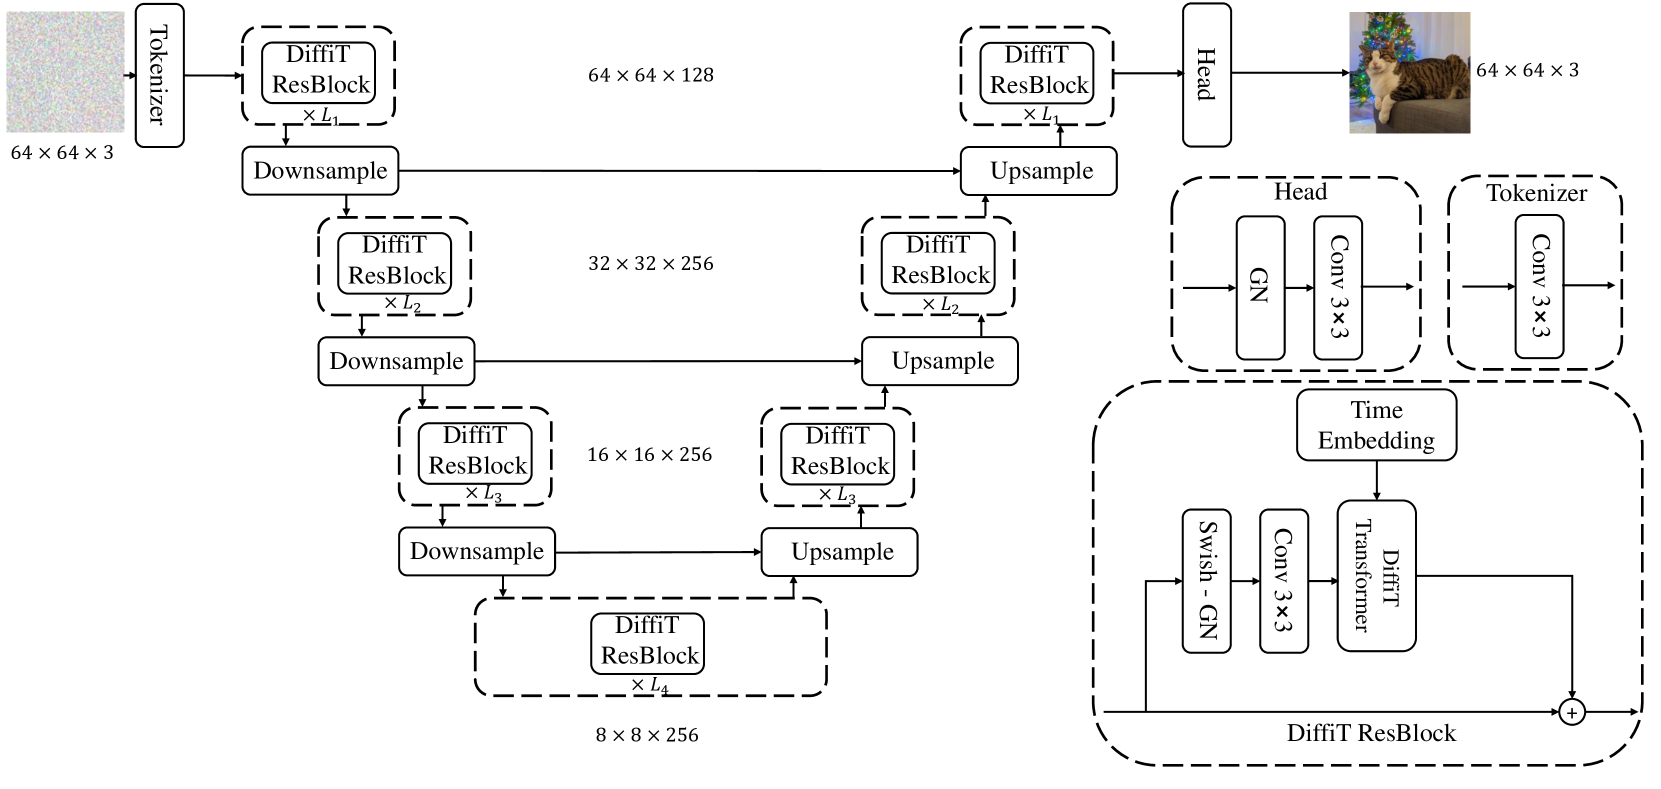
\includegraphics[width=0.9\textwidth]{images/diffit.png}
	\caption[معماری \lr{DiffiT}]{معماری \lr{DiffiT} با بلوک‌های توجه وابسته به زمان (\lr{TMSA}).}
	\label{fig:diffit}
\end{figure}

مدل \lr{LaVin-DiT}\LTRfootnote{Large Vision Diffusion Transformer} ادامه مسیر مقیاس‌پذیری در خانواده \lr{DiT} است و رفتار مدل‌های انتشار بصری را در مقیاس‌های بزرگ‌تر بررسی می‌کند \cite{2411.11505}. این مدل از این جهت در پیشینه قرار می‌گیرد که نشان می‌دهد پرسش اصلی فقط جایگزین کردن \lr{U-Net} با مبدل نیست، بلکه فهم رابطه میان اندازه مدل، حجم محاسبات، کیفیت تولید و هزینه آموزش نیز اهمیت دارد. شکل \ref{fig:lavin_dit} معماری پیشنهادی این مدل را نشان می‌دهد.

\begin{figure}[H]
	\centering
	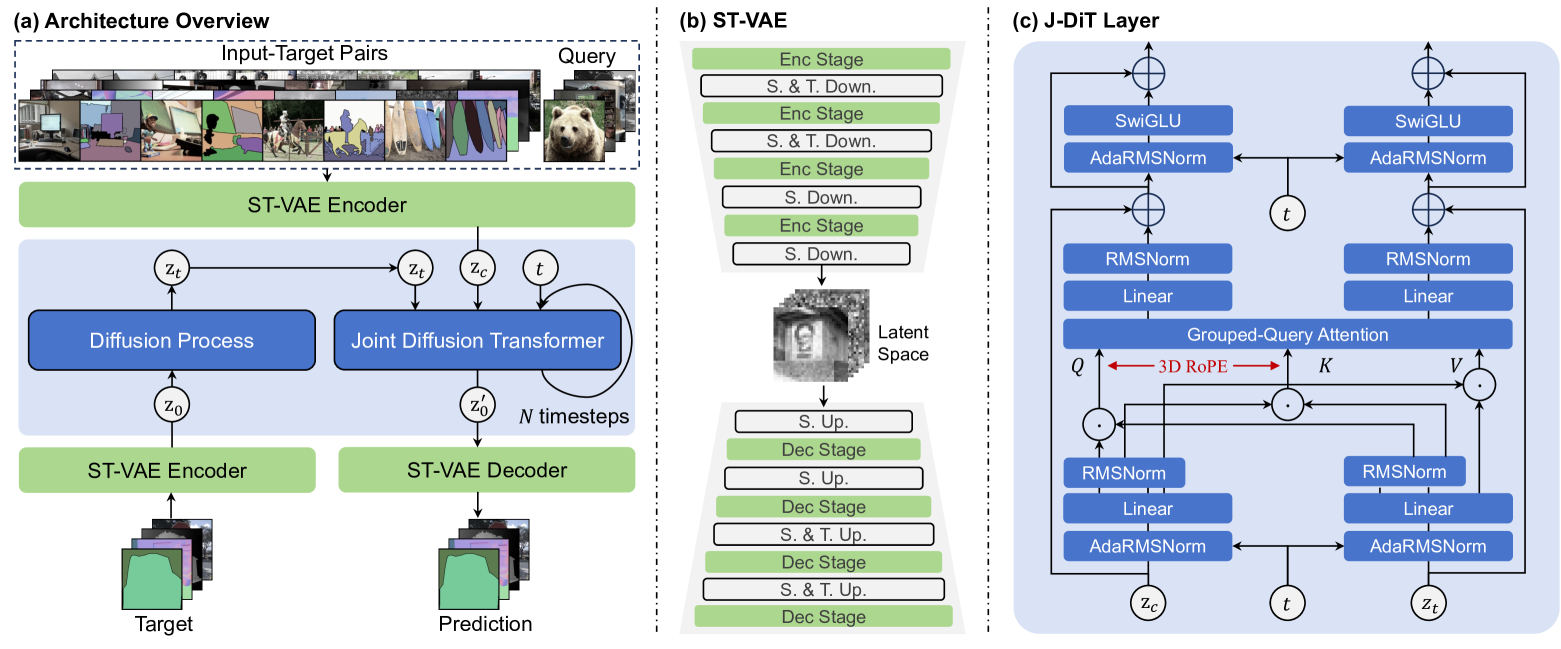
\includegraphics[width=0.9\textwidth]{images/lavin_dit.png}
	\caption[معماری \lr{LaVin-DiT}]{معماری پیشنهادی در \lr{LaVin-DiT} برای بهبود مقیاس‌پذیری \cite{2411.11505}.}
	\label{fig:lavin_dit}
\end{figure}

\lr{LightningDiT} یکی از کارهای جدید در مسیر تقویت مدل‌های انتشار مبتنی بر مبدل است که روی دشواری بهینه‌سازی میان بازسازی نمایش نهان و توان تولید تصویر تمرکز می‌کند \cite{Yao2025LightningDiT}. این کار نشان می‌دهد که در مدل‌های انتشار نهان، کیفیت نهایی فقط به ظرفیت مبدل وابسته نیست، بلکه به تعادل میان کیفیت بازسازی فضای نهان، راهبرد آموزش و مسیر تولید نیز بستگی دارد. از این رو، 
\lr{LightningDiT}
 با بهبود فرایند آموزش مبدل انتشار نهان، به یک مبنای قوی از نظر 
 \lr{FID}
  تبدیل شده است.

\section{روندهای تکمیلی در مدل‌های انتشار مبتنی بر مبدل}

یکی از محورهای اصلی در پیشینه مدل‌های انتشار مبتنی بر مبدل، مسئله مقیاس‌پذیری است. مدل‌های اولیه نشان دادند که با افزایش اندازه شبکه و مقدار محاسبات، کیفیت تولید تصویر بهبود می‌یابد؛ اما این بهبود معمولاً با افزایش شدید هزینه آموزش و استنتاج همراه است. به همین دلیل، پژوهش‌های جدید تلاش کرده‌اند میان ظرفیت مدل، سرعت آموزش و کیفیت نمونه‌های تولیدی تعادل برقرار کنند. برای نمونه، مدل‌های مبتنی بر ماسک‌گذاری و یادگیری با توکن‌های تصویری نشان داده‌اند که می‌توان با کاهش بخشی از محاسبات غیرضروری، آموزش مدل‌های انتشار را سریع‌تر کرد \cite{6822437,2622409}. همچنین چارچوب‌هایی مانند \lr{FiTv2}\LTRfootnote{Flexible Vision Transformer v2}، \lr{EDT}\LTRfootnote{Efficient Diffusion Transformer} و مدل‌های پویای مبدل انتشار، با تغییر طراحی بلوک‌ها، مسیرهای محاسباتی یا سیاست پردازش توکن‌ها تلاش کرده‌اند کیفیت تولید را در کنار کاهش هزینه محاسباتی حفظ کنند \cite{5023251,5439194,7080581,4791247}. در همین امتداد، مدل \lr{Q-DiT}\LTRfootnote{Accurate Post-Training Quantization for Diffusion Transformers} راهکاری برای فشرده‌سازی مدل‌های \lr{DiT} از طریق کوانتیزاسیون پس از آموزش ارائه می‌دهد که در شکل \ref{fig:q_dit} نمایش داده شده است \cite{2406.17343}. این روش با کاهش دقت نمایش وزن‌ها و فعال‌سازی‌ها، بدون نیاز به آموزش مجدد سنگین، کارایی استنتاج را افزایش می‌دهد و نشان می‌دهد که مسئله کارایی تنها به طراحی معماری محدود نیست، بلکه به نحوه نمایش و اجرای پارامترها نیز وابسته است.

\begin{figure}[H]
	\centering
	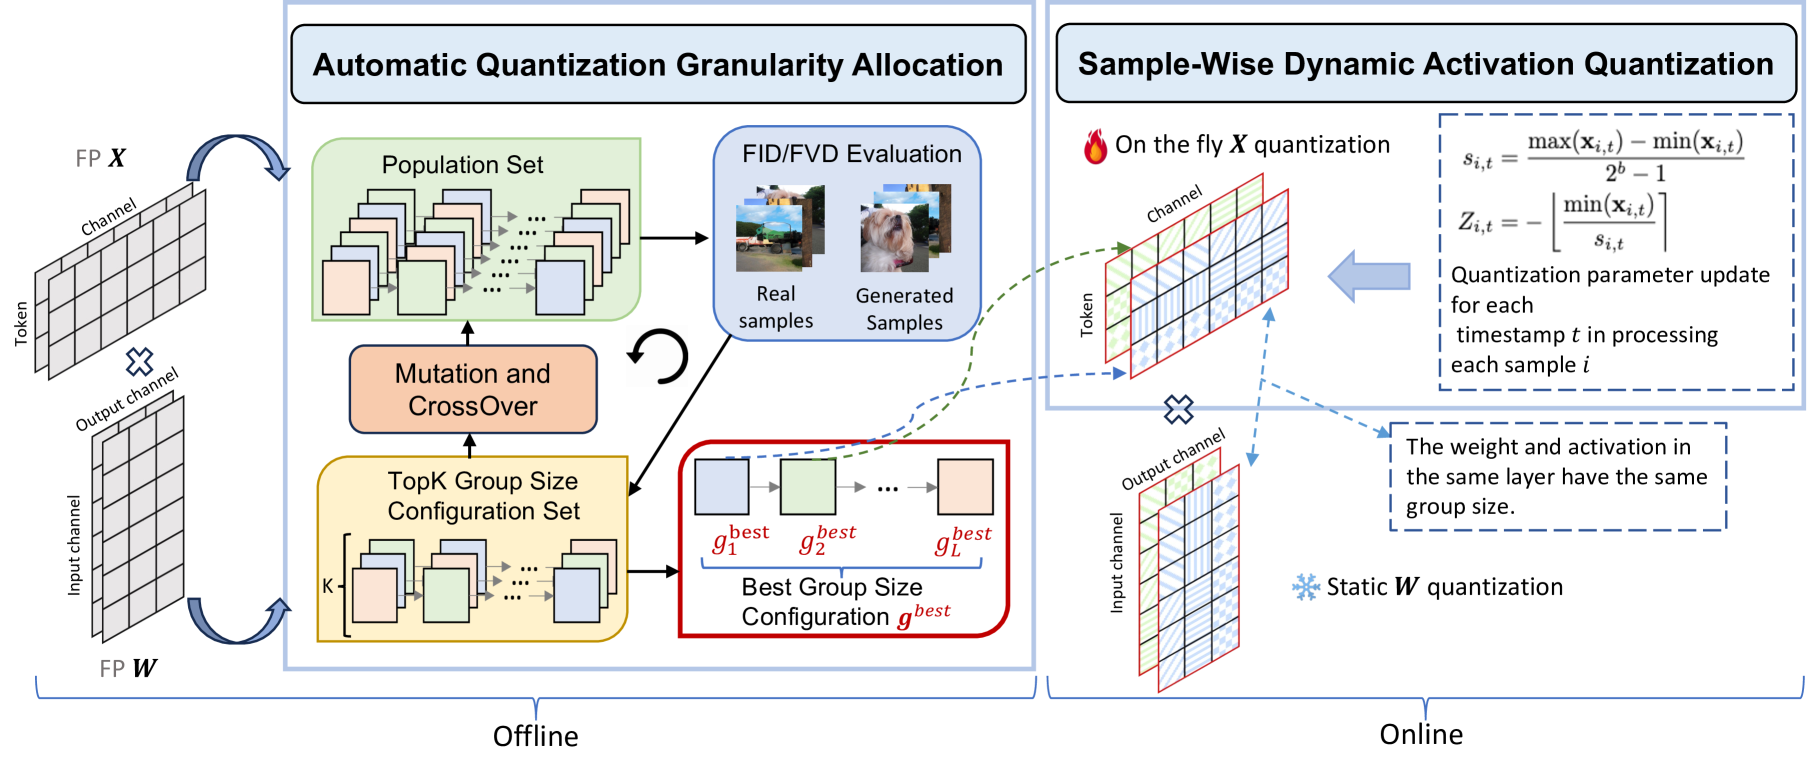
\includegraphics[width=0.9\textwidth]{images/q_dit.png}
	\caption[روش کوانتیزاسیون در \lr{Q-DiT}]{شماتیک روش کوانتیزاسیون در \lr{Q-DiT} \cite{2406.17343}.}
	\label{fig:q_dit}
\end{figure}

در تولید تصویر با وضوح بالا، چالش فقط افزایش تعداد پارامترها نیست؛ بلکه حفظ جزئیات محلی، جلوگیری از اعوجاج و مدیریت وابستگی‌های چندمقیاسی نیز اهمیت دارد. مدل‌هایی مانند \lr{PixArt-Alpha} و نسخه پیشرفته‌تر آن \lr{PixArt-Sigma} با تمرکز بر آموزش کارآمد مبدل‌های انتشار نشان دادند که می‌توان با طراحی مناسب داده، شرط‌گذاری متنی و سازمان‌دهی توکن‌ها، تولید متن-به-تصویر را در وضوح‌های بالا بهبود داد \cite{1031742,chen2024pixartsigma}. همچنین چارچوب‌های مبتنی بر \lr{Rectified Flow}، از جمله مدل مورد استفاده در نسل سوم \lr{Stable Diffusion} و معماری \lr{MM-DiT}\LTRfootnote{Multimodal Diffusion Transformer}، با استفاده از مبدل‌های مقیاس‌پذیر و پردازش جداگانه اطلاعات تصویری و متنی، مسیر دیگری برای تولید تصاویر با کیفیت بالا فراهم کرده‌اند \cite{9168840}. از سوی دیگر، روش‌های چندوضوحی و زمان‌وابسته نشان داده‌اند که کنترل بهتر اطلاعات در سطوح مکانی مختلف می‌تواند به کاهش اعوجاج و بازسازی بهتر ساختارهای تصویری کمک کند \cite{3520873}. این جهت‌گیری‌ها از نظر مفهومی با انگیزه این پژوهش همسو هستند، زیرا معماری پیشنهادی نیز تلاش می‌کند با افزودن شاخه‌ای سبک و وضوح‌بالا، جزئیات مکانی را بدون آموزش مجدد کل مدل تقویت کند.

\subsection{تولید شرطی}
بخش مهم دیگری از پیشینه، به کنترل‌پذیری و شخصی‌سازی مدل‌های انتشار مربوط است. مدل‌های ترکیبی نشان داده‌اند که می‌توان چندین شرط یا مفهوم بصری را در فرایند تولید با یکدیگر ترکیب کرد و از این طریق کنترل معنایی دقیق‌تری بر خروجی به دست آورد \cite{1705308}. روش‌های مبتنی بر مدولاسیون توجه نیز برای تولید متن-به-تصویر متراکم و کنترل‌شده استفاده شده‌اند و نشان داده‌اند که تغییر در نقشه‌های توجه می‌تواند روی جای‌گذاری و انسجام اجزای تصویر اثرگذار باشد \cite{8501335}. همچنین پژوهش‌هایی مانند یادگیری درون‌متنی برای مدل‌های انتشار، تولید شخصی‌سازی‌شده بدون تنظیم زمان آزمون، و تزریق سبک، نشان می‌دهند که سازگار کردن مدل‌های بزرگ با مفهوم یا سبک جدید، یکی از مسائل فعال و مهم در تولید تصویر است \cite{3341281,3521746,3031821}. این روند با بحث هدایت تولید در بخش \ref{sec:ch2-diffusion-frameworks} پیوستگی دارد، زیرا کنترل‌پذیری در عمل به ترکیب شرط‌گذاری، نمونه‌برداری و معماری شبکه حذف نویز وابسته است.

\subsection{کاربردها}
مدل‌های انتشار علاوه بر تصویر دوبعدی، به حوزه‌هایی مانند ویدئو، داده‌های سه‌بعدی و تصویر پزشکی نیز گسترش یافته‌اند. در تولید ویدئو، مدل‌هایی مانند \lr{Video Diffusion Models}، \lr{LaVie} و \lr{Latte} نشان داده‌اند که چالش اصلی، حفظ سازگاری زمانی در کنار کیفیت بصری فریم‌ها است \cite{8313484,8303733,4875773}. در حوزه سه‌بعدی نیز پژوهش‌هایی مانند ویرایش سه‌بعدی فعال‌سازی‌های مدل‌های انتشار یا تولید تصویر استریو نشان می‌دهند که بازنمایی‌های آموخته‌شده در مدل‌های انتشار می‌توانند به فراتر از تولید تصویر دوبعدی تعمیم یابند \cite{9485734,6927085}. همچنین در کاربردهای پزشکی و علمی، تولید تصاویر اخترفیزیکی، سنتز \lr{CT}\LTRfootnote{Computed Tomography} و تحلیل تصاویر بافت‌شناسی نمونه‌هایی از استفاده مدل‌های مولد و مبدل‌ها در دامنه‌های تخصصی هستند \cite{9010310,7223480,4920207}. این گسترش کاربردها نشان می‌دهد که روش‌های سبک و قابل تنظیم، برای انتقال مدل‌های بزرگ به دامنه‌های جدید اهمیت زیادی دارند.

در همین امتداد، مدل \lr{DiT-3D}\LTRfootnote{Three-Dimensional Diffusion Transformer} معماری مبدل‌های انتشار را به تولید \lr{Voxelized Point Clouds} تعمیم می‌دهد \cite{2307.01831}. در این مدل، داده حجمی به پچ‌های سه‌بعدی تقسیم می‌شود و پس از ترکیب با تعبیه‌های موقعیتی سه‌بعدی، به دنباله‌ای از توکن‌ها تبدیل می‌گردد. برای کنترل هزینه محاسباتی ناشی از طول زیاد توکن‌ها در فضای حجمی، \lr{DiT-3D} از توجه پنجره‌ای سه‌بعدی\LTRfootnote{3D Window Attention} استفاده می‌کند و تعاملات را به نواحی محلی محدود می‌سازد. جایگاه این مدل در فصل حاضر بیشتر از زاویه گسترش دامنه کاربرد است، زیرا نشان می‌دهد ایده پچ‌سازی و توجه در \lr{DiT} می‌تواند از تولید تصویر دوبعدی به داده‌های حجمی نیز منتقل شود. این معماری در شکل \ref{fig:dit3d_arch} آمده است.

\begin{figure}[H]
	\centering
	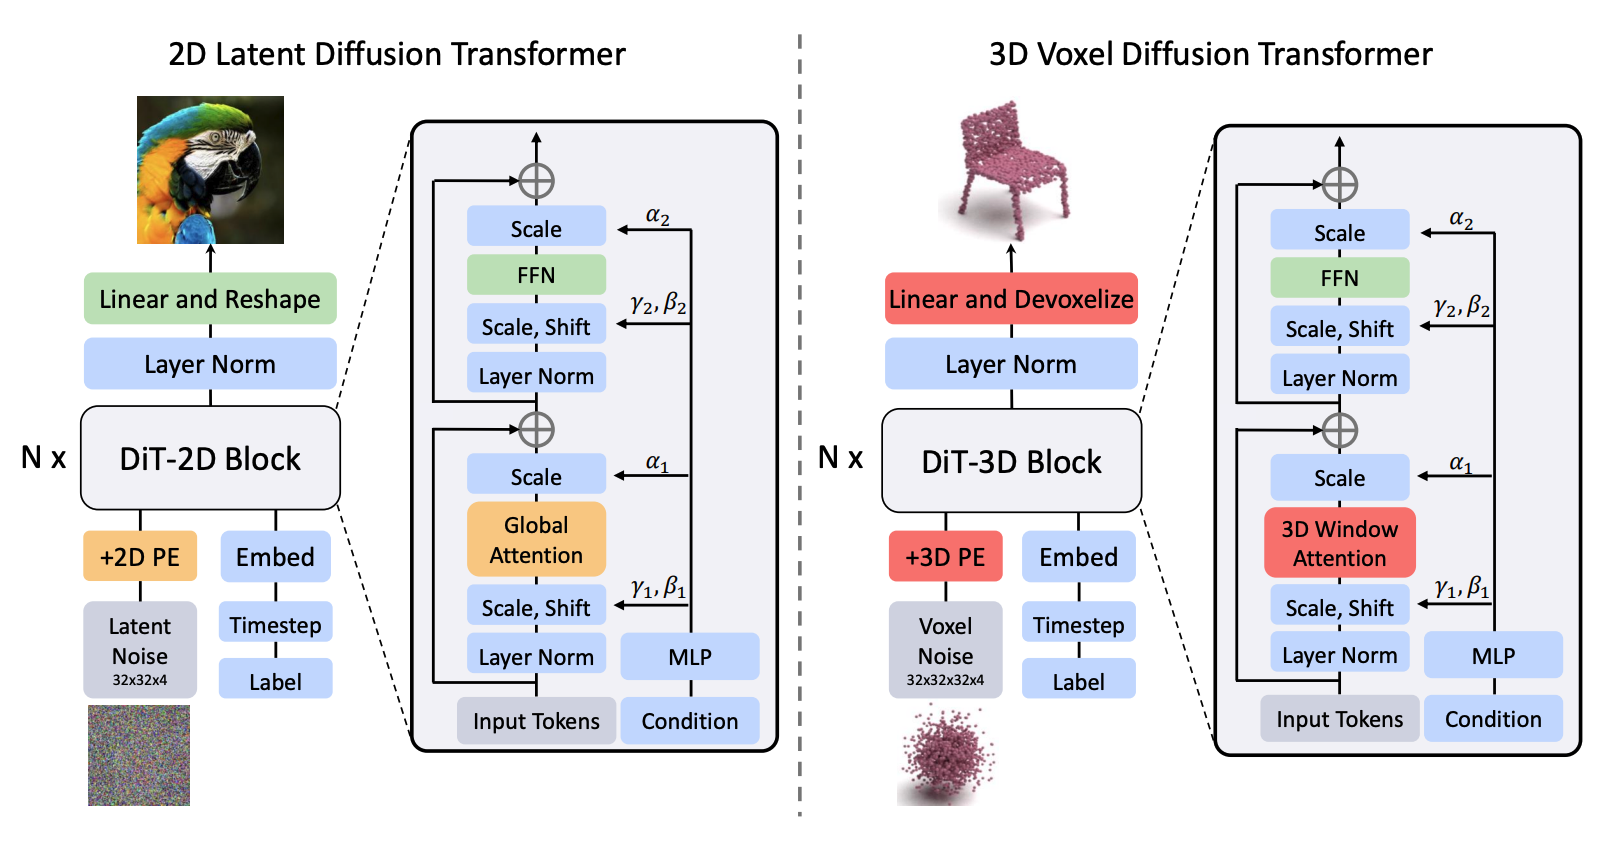
\includegraphics[width=1.0\textwidth]{images/dit_3d.png}
	\caption[معماری \lr{DiT-3D}]{معماری \lr{DiT-3D}: تعمیم مکانیزم پچ‌سازی و توجه به فضای حجمی برای تولید سه‌بعدی \cite{2307.01831}.}
	\label{fig:dit3d_arch}
\end{figure}

\subsection{محلیت و ویژگی‌های ریزدانه}
با وجود قدرت مبدل‌ها در مدل‌سازی وابستگی‌های سراسری، حفظ محلیت و جزئیات ریزدانه همچنان یک مسئله مهم است. پژوهش‌های مربوط به محلیت در مبدل‌های بینایی نشان می‌دهند که نبود سوگیری مکانی محلی می‌تواند در برخی وظایف به ضعف در نمایش بافت‌ها و ساختارهای کوچک منجر شود \cite{0017415}. از سوی دیگر، روش‌هایی که به سازگاری فرکانسی یا تنظیم حافظه‌کارا در مبدل‌های بینایی می‌پردازند، نشان می‌دهند که بخش‌های مختلف طیف فرکانسی و لایه‌های مختلف شبکه نقش یکسانی در انتقال دانش ندارند \cite{7387391,7732706,3649101}.

\section{معماری‌های جریان دوگانه}

استفاده از معماری‌های جریان دوگانه\LTRfootnote{Dual-Stream Architectures} یکی از راهکارهای رایج برای ترکیب اطلاعات سراسری و محلی در پردازش تصویر است. ایده اصلی این رویکرد آن است که یک مسیر شبکه می‌تواند ساختارهای کلی، وابستگی‌های بلندبرد و ویژگی‌های معنایی را مدل کند، در حالی که مسیر دیگر روی جزئیات محلی، لبه‌ها، بافت‌ها و مؤلفه‌های فرکانس بالا تمرکز دارد. برای نمونه، \lr{HRNet}\LTRfootnote{High-Resolution Network} با حفظ نمایش‌های وضوح‌بالا در طول کل فرایند پردازش و تبادل مداوم اطلاعات با شاخه‌های وضوح پایین‌تر، نشان داد که نگه داشتن اطلاعات مکانی دقیق برای وظایفی مانند تشخیص نقاط کلیدی، قطعه‌بندی و بازشناسی بصری اهمیت زیادی دارد \cite{wang2020hrnet}.

شکل \ref{fig:ch2-hrnet-fusion} ایده اصلی \lr{HRNet} را نشان می‌دهد: به‌جای آن‌که شبکه ابتدا نمایش تصویر را به وضوح پایین فشرده و سپس در انتها آن را بازیابی کند، شاخه وضوح‌بالا در تمام مراحل حفظ می‌شود و با شاخه‌های کم‌وضوح‌تر تبادل اطلاعات دارد. این طراحی از نظر مفهومی برای پژوهش حاضر مهم است، زیرا نشان می‌دهد حفظ یک مسیر پرجزئیات می‌تواند مکمل مسیرهای معنایی و کم‌وضوح باشد \cite{wang2020hrnet}.

\begin{figure}[H]
    \centering
    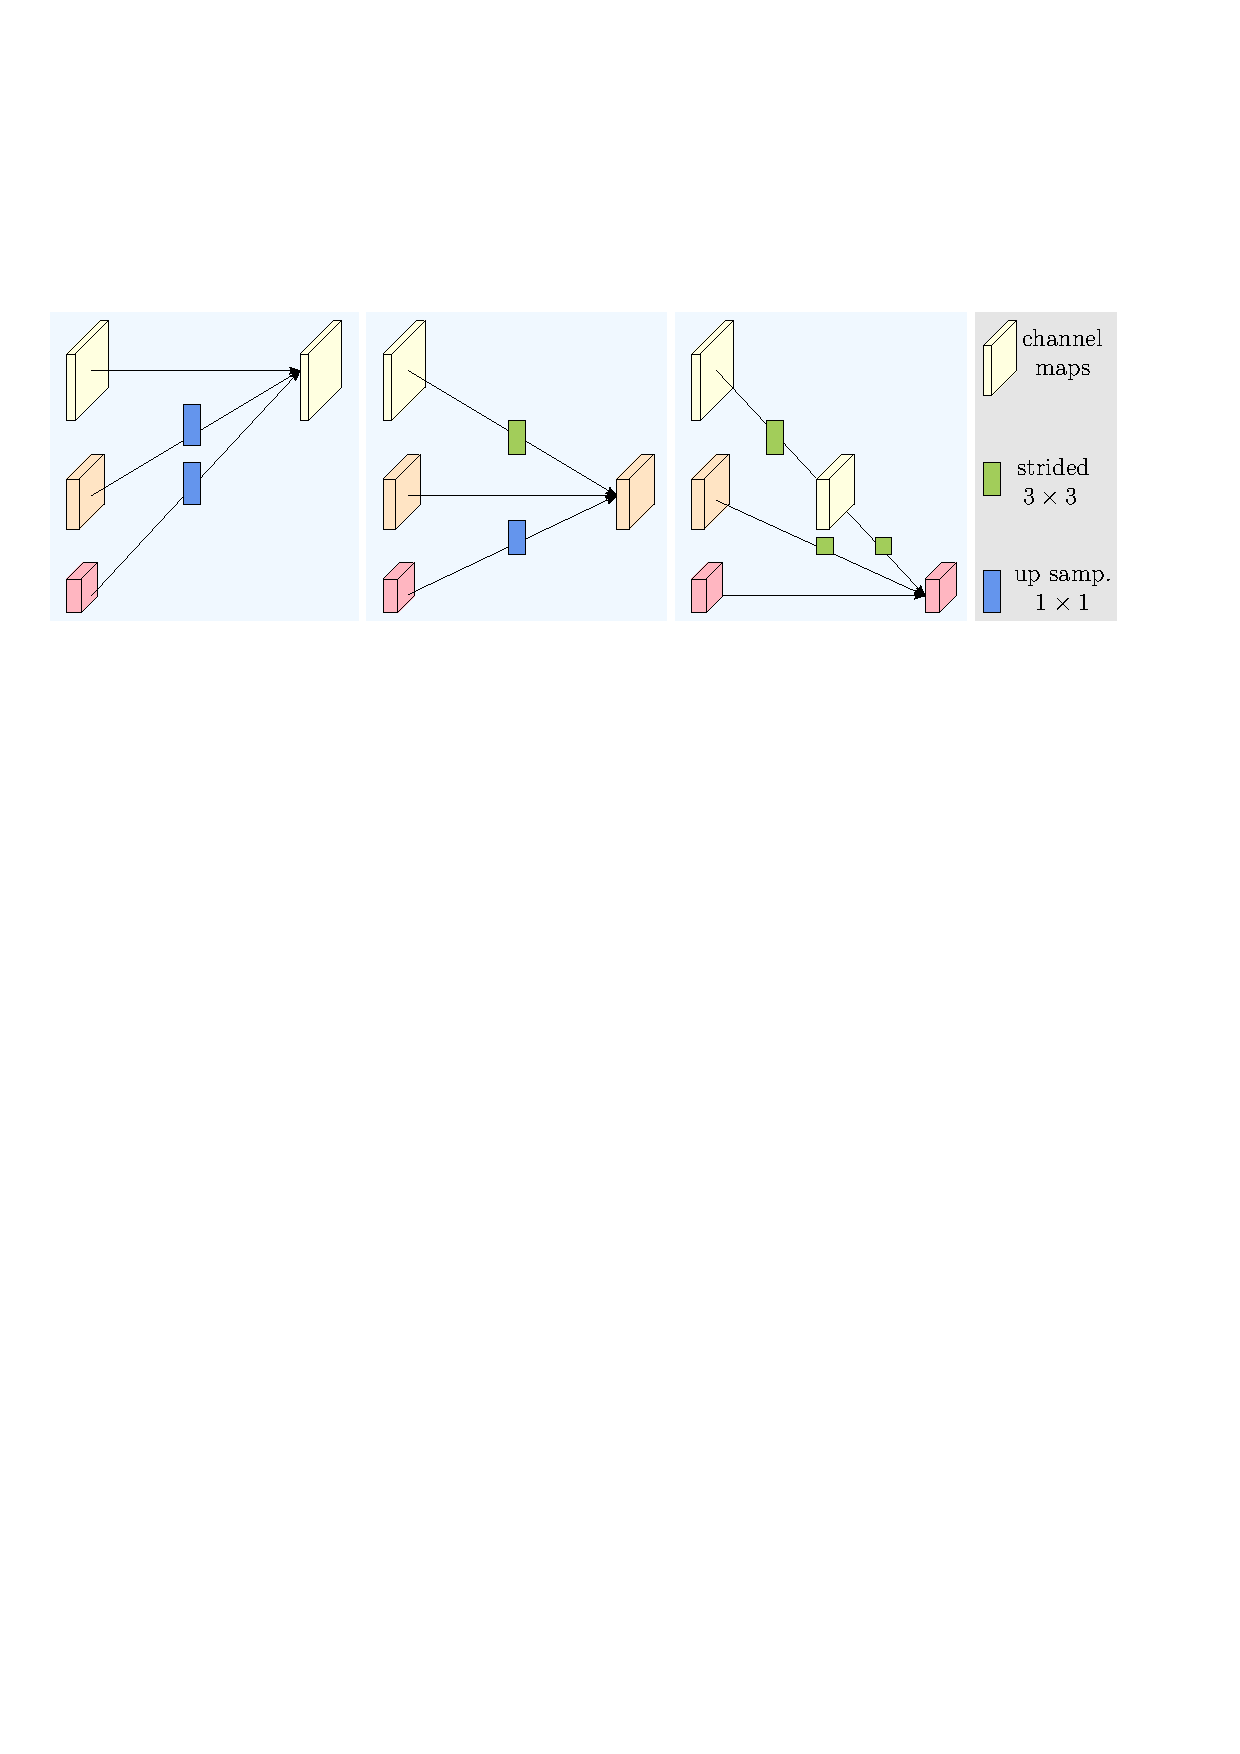
\includegraphics[width=0.92\linewidth]{images/hrnet_multiresolution_fusion.pdf}
    \caption[تجمیع چندوضوحی در \lr{HRNet}]{واحد تجمیع چندوضوحی در \lr{HRNet}: شاخه وضوح‌بالا در کنار شاخه‌های کم‌وضوح‌تر حفظ شده و اطلاعات میان وضوح‌ها به‌صورت مکرر مبادله می‌شود \cite{wang2020hrnet}.}
    \label{fig:ch2-hrnet-fusion}
\end{figure}

در حوزه مبدل‌های بینایی، مدل‌هایی مانند \lr{CrossViT}\LTRfootnote{Cross-Attention Multi-Scale Vision Transformer} این ایده را با استفاده از دو شاخه مبتنی بر اندازه پچ‌های متفاوت پیاده‌سازی کرده‌اند \cite{chen2021crossvit}. در این معماری، که در شکل \ref{fig:ch2-crossvit-architecture} نشان داده شده است، شاخه‌ای با پچ‌های بزرگ‌تر برای دریافت زمینه سراسری و شاخه‌ای با پچ‌های کوچک‌تر برای استخراج جزئیات محلی به کار می‌رود. سپس اطلاعات دو شاخه با سازوکار توجه متقابل میان توکن‌های خلاصه‌ساز مبادله می‌شود. پژوهش‌های مرتبط با طراحی مبدل‌های چندمقیاسی نیز نشان می‌دهند که افزایش دامنه دریافت\LTRfootnote{Receptive Field} در کنار حفظ مسیرهای محلی، برای تحلیل تصویر با وضوح بالا اهمیت کلیدی دارد \cite{3153255,0017415}. همچنین در مدل‌های انتشار مبتنی بر مبدل مانند \lr{U-ViT}، استفاده از مسیرهای چندسطحی و اتصالات بلندبرد، کارایی مشابهی در حفظ اطلاعات جزئیات ایجاد می‌کند \cite{2209.12152}.

\begin{figure}[H]
    \centering
    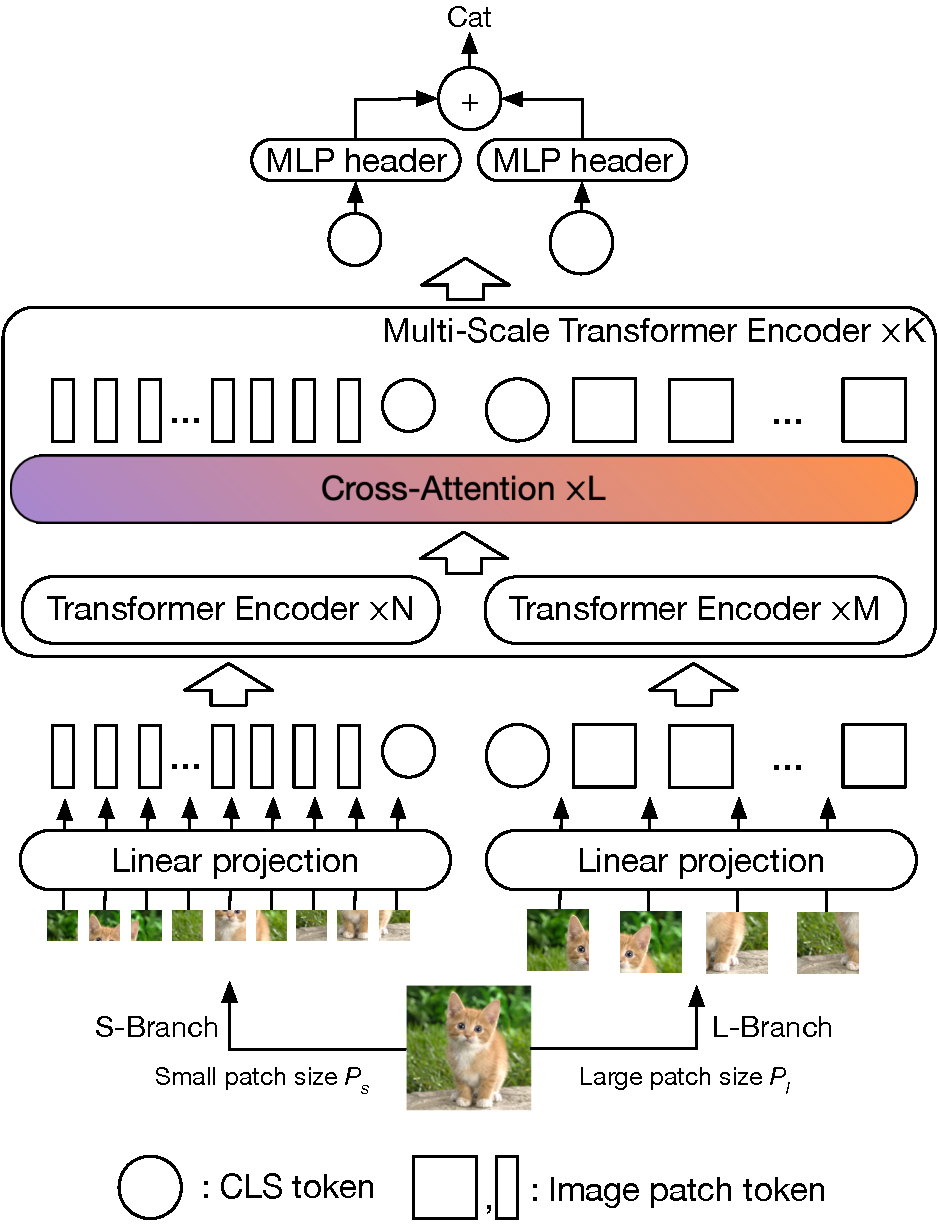
\includegraphics[width=0.96\linewidth]{images/crossvit_architecture.pdf}
    \caption[معماری دوجریانی \lr{CrossViT}]{معماری دوجریانی \lr{CrossViT}: شاخه پچ‌های بزرگ‌تر زمینه سراسری را مدل می‌کند و شاخه پچ‌های کوچک‌تر جزئیات محلی را حفظ می‌کند؛ تبادل اطلاعات میان دو شاخه از طریق توجه متقابل انجام می‌شود \cite{chen2021crossvit}.}
    \label{fig:ch2-crossvit-architecture}
\end{figure}

در \lr{CrossViT} چند راهبرد برای ادغام دو شاخه بررسی شده است: ادغام کامل همه توکن‌ها، ادغام توکن‌های کلاس، ادغام مکانی جفت‌به‌جفت، و ادغام مبتنی بر توجه متقابل. نتیجه مهم این مقایسه آن است که برای انتقال اطلاعات چندمقیاسی الزاماً نیازی به ترکیب پرهزینه همه توکن‌ها نیست؛ گاهی یک توکن خلاصه‌ساز می‌تواند نقش واسط فشرده و کارآمدی میان شاخه‌ها داشته باشد. شکل \ref{fig:ch2-crossvit-fusion} این تفاوت را به‌صورت شماتیک نشان می‌دهد \cite{chen2021crossvit}.

\begin{figure}[H]
    \centering
    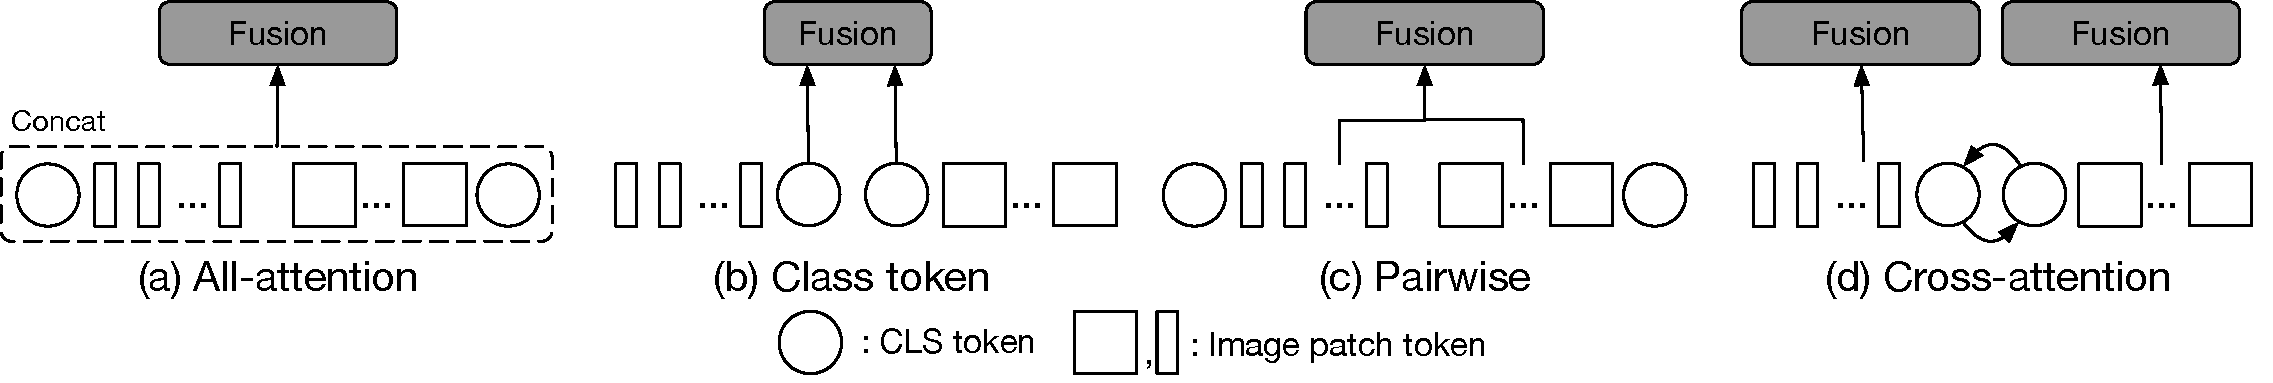
\includegraphics[width=0.9\linewidth]{images/crossvit_fusion_strategies.pdf}
    \caption[\hspace{6pt}راهبردهای ادغام ویژگی در \lr{CrossViT}]{راهبردهای مختلف ادغام ویژگی در \lr{CrossViT}، از ادغام همه توکن‌ها تا توجه متقابل مبتنی بر توکن کلاس \cite{chen2021crossvit}.}
    \label{fig:ch2-crossvit-fusion}
\end{figure}

در سمت مدل‌های انتشار، بازگشت کوتاه به \lr{U-ViT} از زاویه معرفی مدل نیست، بلکه از زاویه حفظ اطلاعات چندسطحی است. همان‌طور که در شکل \ref{fig:uvit} دیده می‌شود، اتصالات بلند میان بلوک‌های ابتدایی و انتهایی مبدل کمک می‌کنند اطلاعات سطح پایین و جزئیات مکانی در مسیر حذف نویز از بین نروند. این نکته، پیوند مستقیمی میان ایده‌های جریان دوگانه و نیاز مدل‌های انتشار به حفظ جزئیات محلی ایجاد می‌کند \cite{2209.12152}.


جدول \ref{tab:ch2-dual-stream-refs} خلاصه می‌کند که هر یک از این معماری‌ها چه نوع مسیری برای حفظ اطلاعات محلی یا چندمقیاسی ایجاد می‌کنند. در هر سه نمونه، یک مسیر کم‌هزینه برای نگه‌داری یا انتقال اطلاعات ریزدانه در کنار مسیر اصلی دیده می‌شود؛ تفاوت در آن است که \lr{HRNet} این کار را با شاخه‌های وضوح متفاوت، \lr{CrossViT} با شاخه‌های پچی متفاوت و توجه متقابل، و \lr{U-ViT} با اتصالات بلند میان لایه‌های مبدل انجام می‌دهد \cite{wang2020hrnet,chen2021crossvit,2209.12152}.

\begin{table}[htbp]
    \centering
    \caption[مقایسه معماری‌های جریان دوگانه]{مقایسه معماری‌های جریان دوگانه}
    \label{tab:ch2-dual-stream-refs}
    \resizebox{\textwidth}{!}{%
    \begin{tabular}{p{0.22\textwidth}p{0.38\textwidth}p{0.32\textwidth}}
        \hline
        \textbf{معماری} & \textbf{مکانیزم اصلی} & \textbf{نوع اطلاعات حفظ‌شده} \\
        \hline
        \lr{HRNet} & نگه‌داری هم‌زمان شاخه‌های وضوح بالا و پایین با تجمیع چندوضوحی تکرارشونده & جزئیات مکانی، لبه‌ها و بافت‌های محلی \\
        \lr{CrossViT} & دو شاخه با اندازه پچ متفاوت و تبادل اطلاعات از طریق توکن‌های کلاس و توجه متقابل & زمینه سراسری در کنار جزئیات ریزدانه مبتنی بر پچ‌های کوچک‌تر \\
        \lr{U-ViT} & اتصال‌های بلند میان بلوک‌های ابتدایی و انتهایی مبدل در شبکه انتشار & اطلاعات سطح پایین و چندمرحله‌ای در مسیر حذف نویز \\
        \hline
    \end{tabular}%
    }
\end{table}

این شواهد نشان می‌دهند که ترکیب هم‌زمان ویژگی‌های درشت‌دانه و ریزدانه می‌تواند برای پردازش تصاویر با وضوح بالا مفید باشد.

\section{تجمیع ویژگی و توکن}
در معماری استاندارد مبدل بینایی، یک توکن ویژه به نام توکن کلاس\LTRfootnote{Class Token} به ابتدای توالی ورودی افزوده می‌شود تا در طول لایه‌های توجه، اطلاعات کل تصویر را به‌صورت فشرده در خود تجمیع کند \cite{Dosovitskiy2020}. این توکن برای وظایفی مانند طبقه‌بندی تصویر مناسب است، زیرا مدل در پایان می‌تواند بازنمایی سراسری تصویر را از آن استخراج کند. با این حال، در معماری‌های چندشاخه یا جریان دوگانه، یک توکن سراسری واحد همیشه برای حفظ جزئیات محلی کافی نیست؛ زیرا ممکن است هنگام فشرده‌سازی کل تصویر، بخشی از اطلاعات ریزدانه و مکانی از دست برود.

راهبرد توکن‌های کلاس محلی بر این ایده استوار است که به‌جای استفاده از یک توکن خلاصه‌ساز برای کل تصویر، می‌توان برای هر ناحیه یا گروهی از توکن‌ها یک توکن خلاصه‌ساز جداگانه تعریف کرد. اگر نمایش محلی توکن‌ها را با $X_l$ نشان دهیم، توکن محلی می‌تواند در نقش «پرس‌وجو» ($Q$) عمل کند و اطلاعات مهم را از «کلیدها» ($K$) و «مقادیر» ($V$) متناظر با همان گروه استخراج کند. محاسبه توجه در این حالت همان رابطه \ref{eq:scaled-dot-product-attention} است، اما $Q$، $K$ و $V$ فقط از توکن‌های همان گروه محلی ساخته می‌شوند \cite{Dosovitskiy2020,chen2021crossvit}.
سازوکارهای مشابه در معماری‌هایی مانند \lr{CrossViT} برای تبادل اطلاعات میان شاخه‌های چندمقیاسی استفاده شده‌اند؛ نمونه‌ای از این سازوکار در شکل \ref{fig:ch2-crossvit-ca-module} آمده است \cite{chen2021crossvit}.

\begin{figure}[H]
    \centering
    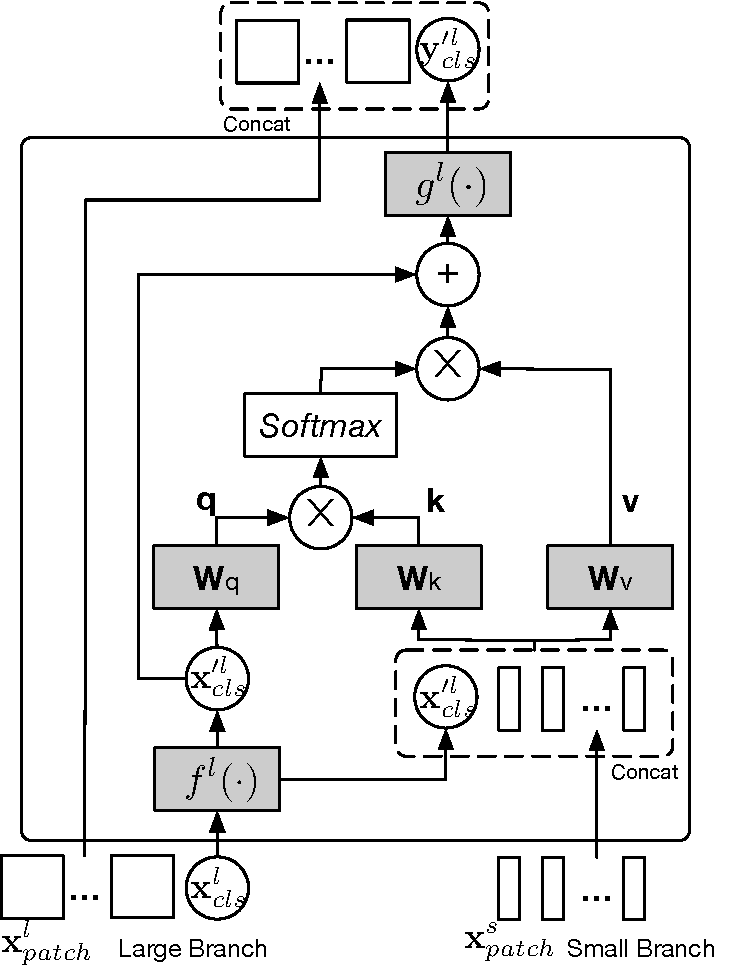
\includegraphics[width=0.9\linewidth]{images/crossvit_cross_attention_module.pdf}
    \caption[\hspace{6pt}ماژول توجه متقابل در \lr{CrossViT}]{ماژول توجه متقابل در \lr{CrossViT}: توکن کلاس یک شاخه نقش پرس‌وجو را دارد و اطلاعات را از توکن‌های شاخه دیگر دریافت می‌کند \cite{chen2021crossvit}.}
    \label{fig:ch2-crossvit-ca-module}
\end{figure}

\section{روش‌های تنظیم دقیق}

\label{sec:full_finetuning} تنظیم دقیق کامل به عنوان رویکرد پایه در تغییر رفتار مدل‌های بزرگ، شامل آزادسازی و به‌روزرسانی تمام پارامترهای شبکه در طول آموزش روی وظیفه یا دامنه هدف است. این فرآیند نسبت به روش‌های تنظیم دقیق پارامتر-کارا، پیچیدگی و هزینه بسیار بیشتری دارد چرا که شبکه‌های امروزی ممکن است دارای میلیاردها پارامتر باشند. همین ویژگی موجب مصرف بالای حافظه \lr{GPU}\LTRfootnote{Graphics Processing Unit}،
 نیاز به ذخیره‌سازی فعال‌سازی‌ها برای کل لایه‌ها، و افزایش زمان هر گام یادگیری می‌شود 
 \cite{5294562}.

\subsection{تنظیم دقیق پارامتر-کارا}
\label{sec:efficient_parameter_finetuning} تنظیم دقیق پارامتر-کارا در سال‌های اخیر به عنوان پاسخی عملی به محدودیت‌های زمان و منابع موردنیاز برای آموزش مدل‌های بزرگ مطرح شده است. ایده اصلی کاهش تعداد پارامترهایی است که طی فرآیند تنظیم دقیق به‌روز می‌شوند تا فشار حافظه، هزینه محاسباتی و مدت زمان آموزش کمتر شود، در حالی که کیفیت خروجی در سطح رقابتی باقی بماند \cite{8409325}. 
در این رویکردها بخش اعظم وزن‌های شبکه ثابت نگه داشته شده و تنها مجموعه کوچکی از پارامترهای افزوده‌شده یا انتخاب‌شده برای یادگیری آزاد هستند. 
\lr{FineDiffusion} یک روش تنظیم دقیق پارامتر-کارا برای تولید تصویر شرطی ریزدانه است که مسئله مقیاس‌پذیری تولید کلاسی را در تعداد زیاد کلاس‌ها بررسی می‌کند \cite{Pan2024FineDiffusion}. ایده اصلی این روش آن است که برای سازگار کردن مدل انتشار با کلاس‌های ریزدانه، لازم نیست همه وزن‌های شبکه آزاد شوند؛ در عوض می‌توان بخش محدودی از پارامترهای مؤثر بر شرط‌گذاری و تطبیق آماری مدل را به‌روزرسانی کرد. این بخش‌ها شامل تعبیه‌های کلاسی، بایاس‌ها و پارامترهای مرتبط با نرمال‌سازی هستند؛ یعنی اجزایی که رفتار شرطی مدل را تغییر می‌دهند، اما بدنه اصلی تولیدکننده را تا حد زیادی حفظ می‌کنند.

% \section{جمع‌بندی}
در این فصل، پیشینه پژوهش‌های مرتبط با معماری پیشنهادی از چهار زاویه بررسی شد. نخست، چارچوب‌های اصلی مدل‌های انتشار و مسیر حرکت آن‌ها به سمت مدل‌های مبتنی بر مبدل توضیح داده شد و نمونه‌هایی مانند \lr{GenViT}، \lr{U-ViT}، \lr{DiT}، \lr{DiffiT}، \lr{LaVin-DiT} و \lr{LightningDiT} نشان دادند که مبدل‌ها می‌توانند به بدنه اصلی مدل‌های انتشار تبدیل شوند. دوم، روندهای تکمیلی حوزه نشان دادند که مقیاس‌پذیری، کارایی، شرط‌پذیری و حفظ جزئیات محلی همچنان چالش‌های مهم این خانواده از مدل‌ها هستند. سوم، معماری‌های جریان دوگانه و چندوضوحی مانند \lr{HRNet} و \lr{CrossViT} نشان دادند که ترکیب یک مسیر سراسری با مسیری محلی می‌تواند راهکاری مؤثر برای حفظ جزئیات ریزدانه باشد. چهارم، روش‌های تنظیم دقیق پارامتر-کارا، به‌ویژه \lr{FineDiffusion}، نشان دادند که می‌توان بدون به‌روزرسانی کامل مدل پایه، مسیرهای جدیدی برای سازگارسازی و تزریق ویژگی ایجاد کرد \cite{0214306,2212.09748,wang2020hrnet,chen2021crossvit,8409325,Pan2024FineDiffusion}.

% بر این اساس، شکاف پژوهشی این پایان‌نامه در نقطه اتصال این چهار محور قرار می‌گیرد: استفاده از یک بدنه اصلی \lr{DiT} برای حفظ دانش سراسری، افزودن یک شاخه وضوح‌بالا برای استخراج ویژگی‌های محلی، به‌کارگیری توکن‌های کلاس محلی برای تجمیع هوشمند ویژگی‌ها، و آموزش تنها بخش کوچکی از پارامترها برای کاهش هزینه تنظیم دقیق. فصل بعد معماری پیشنهادی \lr{DuoDiT} را بر پایه همین منطق معرفی می‌کند.

\chapter{معماری پیشنهادی: \lr{DuoDiT}}
\label{ch:proposed_method}

در این فصل، معماری پیشنهادی این پژوهش با عنوان \lr{DuoDiT} معرفی می‌شود. هدف این معماری، تنظیم دقیق پارامتر-کارای مدل‌های انتشار مبتنی بر مبدل (\lr{DiT}) برای کلاس‌ها یا دامنه‌های هدف است؛ به گونه‌ای که بدون به‌روزرسانی کامل بدنه اصلی، مسیر جداگانه‌ای برای استخراج و تزریق ویژگی‌های محلی فراهم شود. چالش اصلی در این مسئله آن است که تنظیم دقیق کامل مدل‌های بزرگ هزینه محاسباتی و حافظه‌ای بالایی دارد و در عین حال، روش‌های بسیار فشرده ممکن است برای تغییر بازنمایی‌های مکانی و حفظ جزئیات محلی کافی نباشند \cite{2212.09748,8409325}.

معماری \lr{DuoDiT} بر یک ساختار دوجریانی (\lr{Dual-Stream Architecture}) استوار است. جریان نخست، بدنه اصلی \lr{DiT} است که وزن‌های آن ثابت نگه داشته می‌شود و نقش حفظ دانش پیش‌آموزش‌دیده و ساختار معنایی تصویر را بر عهده دارد. جریان دوم، شاخه وضوح‌بالا یا شاخه \lr{x2} است که با اندازه پچ کوچک‌تر عمل می‌کند و ویژگی‌های ریزدانه‌تری تولید می‌کند. روش اصلی این پژوهش برای هم‌تراز کردن خروجی شاخه \lr{x2} با توکن‌های بدنه اصلی، مکانیزم «توکن‌های کلاس محلی» است؛ به این معنا که برای هر گروه محلی از چهار توکن وضوح‌بالا، یک توکن خلاصه‌ساز یادگیرنده تولید می‌شود و خروجی همین توکن به‌عنوان نماینده آن ناحیه به جریان اصلی افزوده می‌گردد \cite{2212.09748,chen2021crossvit,Dosovitskiy2020}.

\section{معماری مدل}
سیستم پیشنهادی از دو بخش اصلی تشکیل شده است. بخش نخست، \textbf{جریان بدنه اصلی منجمد (\lr{Frozen Backbone})} است که همان مدل \lr{DiT-XL/2} بوده و وزن‌های آن، شامل تعبیه‌ساز پچ، بلوک‌های مبدل و لایه‌های شرط‌گذاری اصلی، ثابت نگه داشته می‌شوند. این جریان بازنمایی اصلی نویز ورودی، زمان و برچسب کلاس را تولید می‌کند. بخش دوم، \textbf{جریان وضوح‌بالا (\lr{x2 Stream})} است که شامل تعبیه‌ساز پچ با اندازه کوچک‌تر، بلوک مبدل شاخه کمکی، مکانیزم تجمیع مبتنی بر توکن کلاس محلی و پروجکشن‌های تطبیق ابعاد است. معماری از نظر طراحی امکان افزودن شرط‌گذاری \lr{FiLM} را نیز دارد، اما این مؤلفه در آموزش اصلی \lr{ImageNet-1K} فعال نشده است \cite{2212.09748,Dosovitskiy2020,perez2018film}.

در پیاده‌سازی نهایی این پژوهش، ادغام دو جریان به‌صورت جمع باقی‌مانده پس از آخرین بلوک مبدل بدنه اصلی انجام می‌شود؛ این همان تنظیمی است که در فصل آزمایش‌ها با نام \lr{x2\_final\_fuse} گزارش شده است. بنابراین، گزینه‌هایی مانند ادغام متناوب در چندین بلوک، بخشی از فضای طراحی محسوب می‌شوند اما روش اصلی گزارش‌شده در این پایان‌نامه ادغام نهایی است \cite{Vaswani2017,2212.09748}.

شکل \ref{fig:proposed_architecture_overview} نمای کلی جریان معماری پیشنهادی را نشان می‌دهد. در این نما، مسیر بدنه اصلی \lr{DiT} در کنار شاخه وضوح‌بالا قرار گرفته و نقش مکانیزم توکن‌های کلاس محلی در فشرده‌سازی و انتقال ویژگی‌های شاخه \lr{x2} به جریان اصلی مشخص شده است.

\begin{figure}[H]
    \centering
    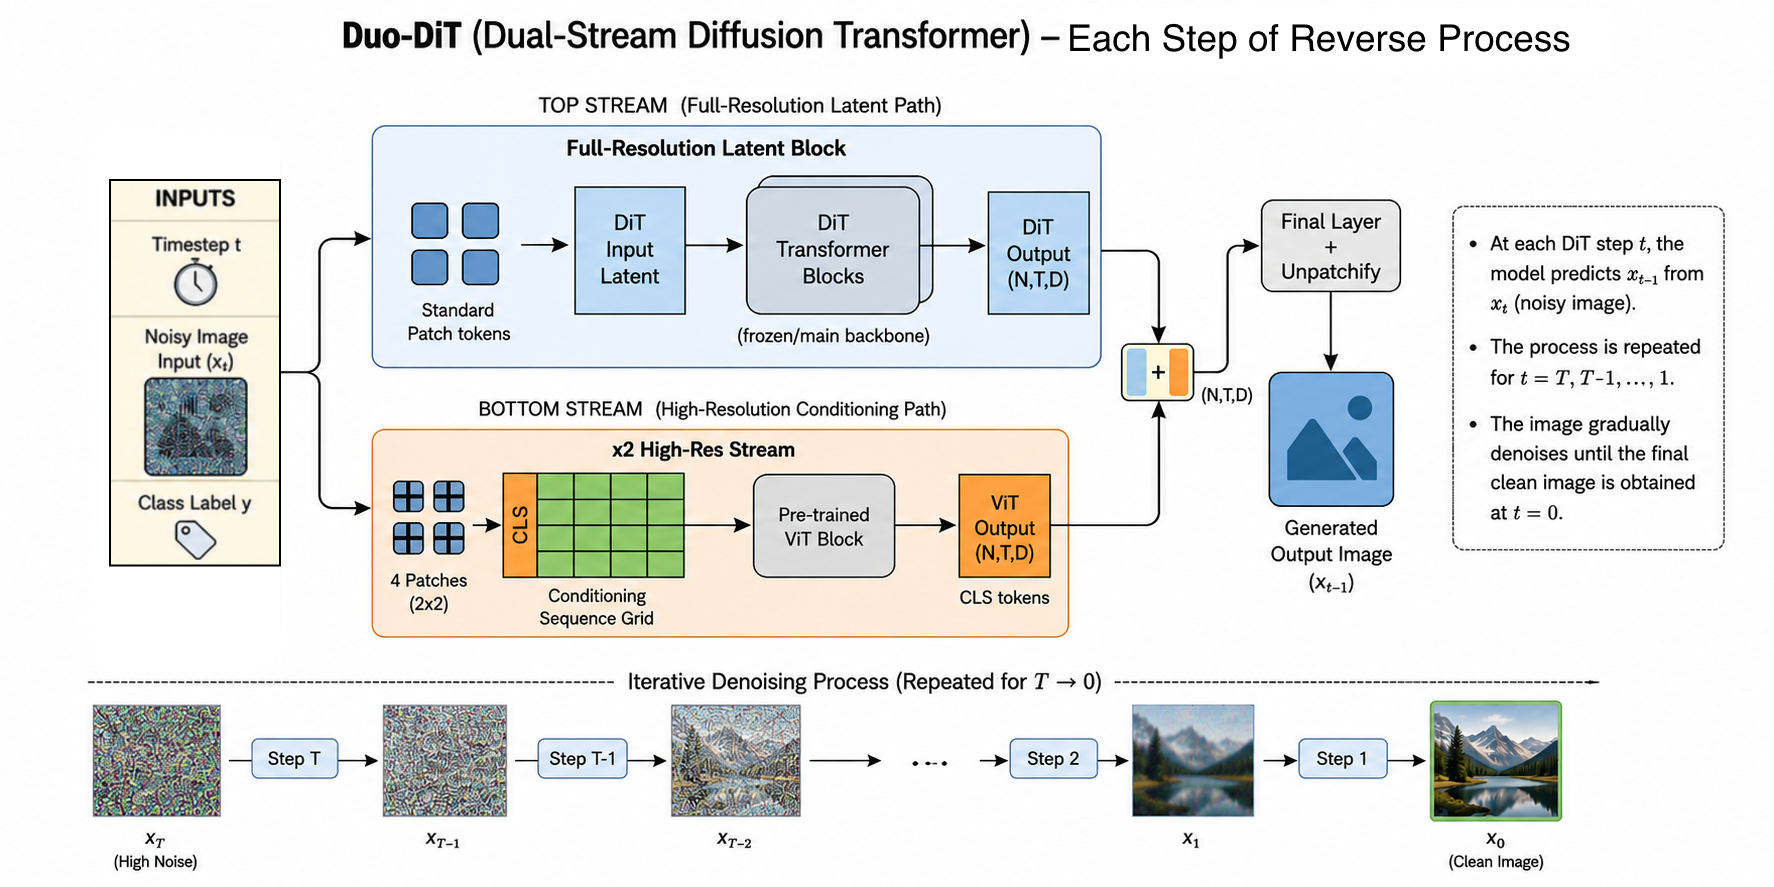
\includegraphics[width=0.95\linewidth]{images/duodit-arch-overview.drawio.png}
    \caption[نمای کلی معماری پیشنهادی مبتنی بر توکن‌های کلاس محلی]{نمای کلی معماری پیشنهادی و جریان تجمیع ویژگی مبتنی بر توکن‌های کلاس محلی. شاخه وضوح‌بالا ویژگی‌های ریزدانه را استخراج کرده و توکن‌های کلاس محلی، اطلاعات هر گروه از توکن‌ها را برای ادغام با بدنه اصلی \lr{DiT} فشرده می‌کنند.}
    \label{fig:proposed_architecture_overview}
\end{figure}

\subsection{تعبیه‌ساز پچ با وضوح بالا}
در مدل استاندارد \lr{DiT-XL/2}، ورودی نهان به پچ‌های $2 \times 2$ تقسیم می‌شود. در شاخه \lr{x2}، برای افزایش تفکیک مکانی اولیه، اندازه پچ برابر $p'=1$ در نظر گرفته شده است. اگر تعداد توکن‌های شاخه اصلی برابر $T$ باشد، شاخه \lr{x2} چهار برابر آن، یعنی $4T$ توکن تولید می‌کند. این اختلاف تعداد توکن‌ها باعث می‌شود پیش از ادغام با جریان اصلی، یک مرحله هم‌ترازسازی و کاهش طول توالی لازم باشد. روش اصلی این هم‌ترازسازی در این پژوهش، مکانیزم توکن کلاس محلی است \cite{2212.09748,Dosovitskiy2020}.

\subsection{روش‌های تجمیع ویژگی}
سه راهبرد ساده‌تر برای کاهش طول توالی شاخه \lr{x2} در نظر گرفته شده‌اند تا در فصل آزمایش‌ها با روش توکن کلاس محلی مقایسه شوند. این راهبردها بخشی از معماری نهایی نیستند، بلکه نقش مبناهای مقایسه‌ای را دارند \cite{726791,chen2021crossvit}.

\subsubsection{تجمیع با پروجکشن خطی}
در این روش، برای کاهش ابعاد و ادغام ویژگی‌های شاخه \lr{x2} با بدنه اصلی، از مکانیسم الحاق و پروجکشن خطی استفاده می‌شود. برای هر ناحیه $2 \times 2$ از تصویر که متناظر با ۴ توکن در شاخه با وضوح بالا است، ویژگی‌ها به صورت برداری به یکدیگر متصل می‌شوند \cite{2212.09748,chen2021crossvit}.
فرض کنید $Z_{x2}$ ویژگی‌های ورودی باشند. برای هر موقعیت $i$، چهار توکن $z_{4i}, z_{4i+1}, z_{4i+2}, z_{4i+3}$ وجود دارد. خروجی تجمیع شده $z'_i$ به صورت زیر محاسبه می‌شود:
\begin{equation}
    \label{eq:linear-projection-aggregation}
    z'_i = W \cdot \text{Concat}(z_{4i}, z_{4i+1}, z_{4i+2}, z_{4i+3}) + b
\end{equation}
\begin{figure}[H]
    \centering
    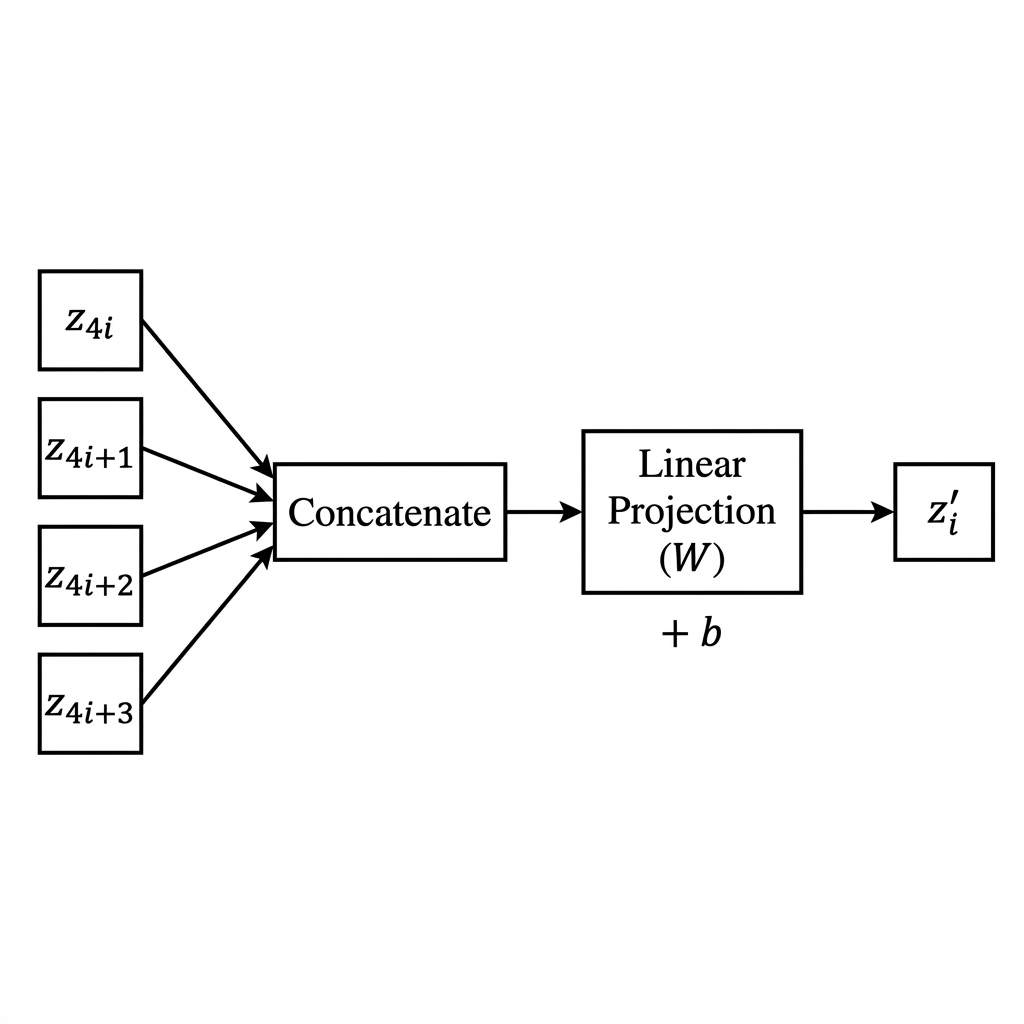
\includegraphics[width=0.9\linewidth]{images/linear_projection_aggregation.png}
    \caption[تجمیع ویژگی با پروجکشن خطی]{نمای شماتیک از تجمیع ویژگی با استراتژی پروجکشن خطی. انطباق ۴ توکن ورودی به یک توکن خروجی با استفاده از پروجکشن خطی.}
    \label{fig:linear_proj}
\end{figure}
در این رابطه، $W$ ماتریس وزن لایه خطی است که ابعاد فضای ویژگی ادغام شده را به ابعاد فضای هدف تطبیق می‌دهد. شکل \ref{fig:linear_proj} این نگاشت چهار توکن ورودی به یک توکن خروجی را به‌صورت شماتیک نشان می‌دهد.

\subsubsection{تجمیع با \lr{Max Pooling}}
در این رویکرد، برای استخراج ویژگی نهایی از هر پچ، از عملیات \lr{Max Pooling} استفاده می‌شود. این روش بر این فرض استوار است که بیشینه مقدار فعالیت در هر کانال ویژگی، بیانگر برجسته‌ترین اطلاعات آن ناحیه است \cite{726791}.
برای هر گروه ۴ تایی از توکن‌ها که مربوط به یک پچ از تصویر اصلی هستند، مقدار بیشینه در هر بعد ویژگی محاسبه می‌شود:
\begin{equation}
    \label{eq:max-pooling-aggregation}
    z'_{i,j} = \max(z_{4i,j}, z_{4i+1,j}, z_{4i+2,j}, z_{4i+3,j})
\end{equation}
در اینجا $z'_{i,j}$ مقدار $j$-امین ویژگی از $i$-امین توکن خروجی است. این عملیات بدون استفاده از پارامترهای یادگیرنده انجام می‌شود.

\subsubsection{تجمیع با \lr{Min Pooling}}
این روش مشابه رویکرد \lr{Max Pooling} است، با این تفاوت که از عملیات \lr{Min Pooling} استفاده می‌کند. در اینجا تمرکز بر کمینه مقدار سیگنال در هر زیر-ناحیه است.
رابطه ریاضی این تبدیل به صورت زیر تعریف می‌شود:
\begin{equation}
    \label{eq:min-pooling-aggregation}
    z'_{i,j} = \min(z_{4i,j}, z_{4i+1,j}, z_{4i+2,j}, z_{4i+3,j})
\end{equation}
\begin{figure}[H]
    \centering
    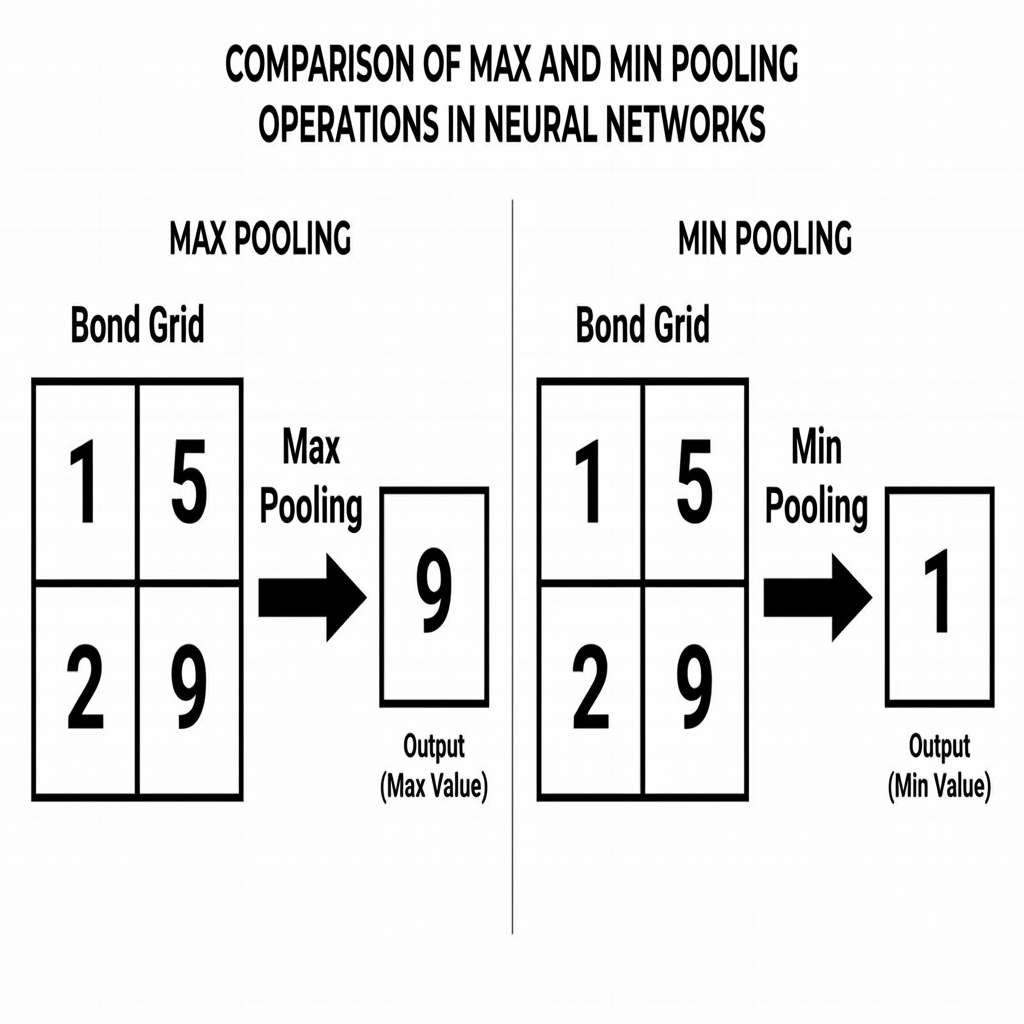
\includegraphics[width=0.9\linewidth]{images/pooling_operations.png}
    \caption[مقایسه \lr{Max Pooling} و \lr{Min Pooling}]{مقایسه عملیات \lr{Max Pooling} و \lr{Min Pooling}. در سمت چپ، انتخاب بیشینه مقدار و در سمت راست، انتخاب کمینه مقدار مشاهده می‌شود.}
    \label{fig:pooling_ops}
\end{figure}
این رویکرد نیز همانند روش بیشینه، یک عملیات ثابت و بدون وزن‌های قابل آموزش است که اطلاعات مکانی را با انتخاب اکسترمم‌ها فشرده‌سازی می‌کند. شکل \ref{fig:pooling_ops} تفاوت انتخاب بیشینه و کمینه را در این نوع تجمیع نشان می‌دهد.

\subsection{روش تجمیع ویژگی با توکن}
\label{sec:local_cls}
در معماری نهایی \lr{DuoDiT}، کاهش طول توالی شاخه \lr{x2} به‌صورت یک عملیات یادگیرنده انجام می‌شود. در روش‌های ثابت مانند میانگین‌گیری یا بیشینه‌گیری، قاعده فشرده‌سازی مستقل از محتوای تصویر است؛ در نتیجه، همه گروه‌های محلی با یک قانون یکسان خلاصه می‌شوند. در مقابل، توکن کلاس محلی یک بردار یادگیرنده است که همراه با توکن‌های هر ناحیه پردازش می‌شود و می‌تواند بر اساس الگوی محلی همان ناحیه، بازنمایی فشرده‌تری تولید کند \cite{726791,Dosovitskiy2020,chen2021crossvit}.

در مدل‌های استاندارد \lr{ViT}، یک توکن کلاس سراسری برای خلاصه‌سازی کل تصویر به کار می‌رود. در این پژوهش، همین ایده در مقیاس محلی استفاده شده است: هر چهار توکن شاخه \lr{x2} که متناظر با یک توکن شاخه اصلی هستند، همراه با یک توکن کلاس محلی وارد بلوک پردازشی می‌شوند و خروجی توکن کلاس به عنوان نماینده همان ناحیه انتخاب می‌شود. بنابراین، خروجی شاخه \lr{x2} از $4T$ توکن به $T$ توکن کاهش می‌یابد و از نظر طول توالی با بدنه اصلی هم‌راستا می‌شود. شکل \ref{fig:local_cls} سازوکار گروه‌بندی توکن‌ها و استخراج خروجی محلی را نمایش می‌دهد \cite{Dosovitskiy2020,chen2021crossvit}.

\begin{figure}[H]
    \centering
    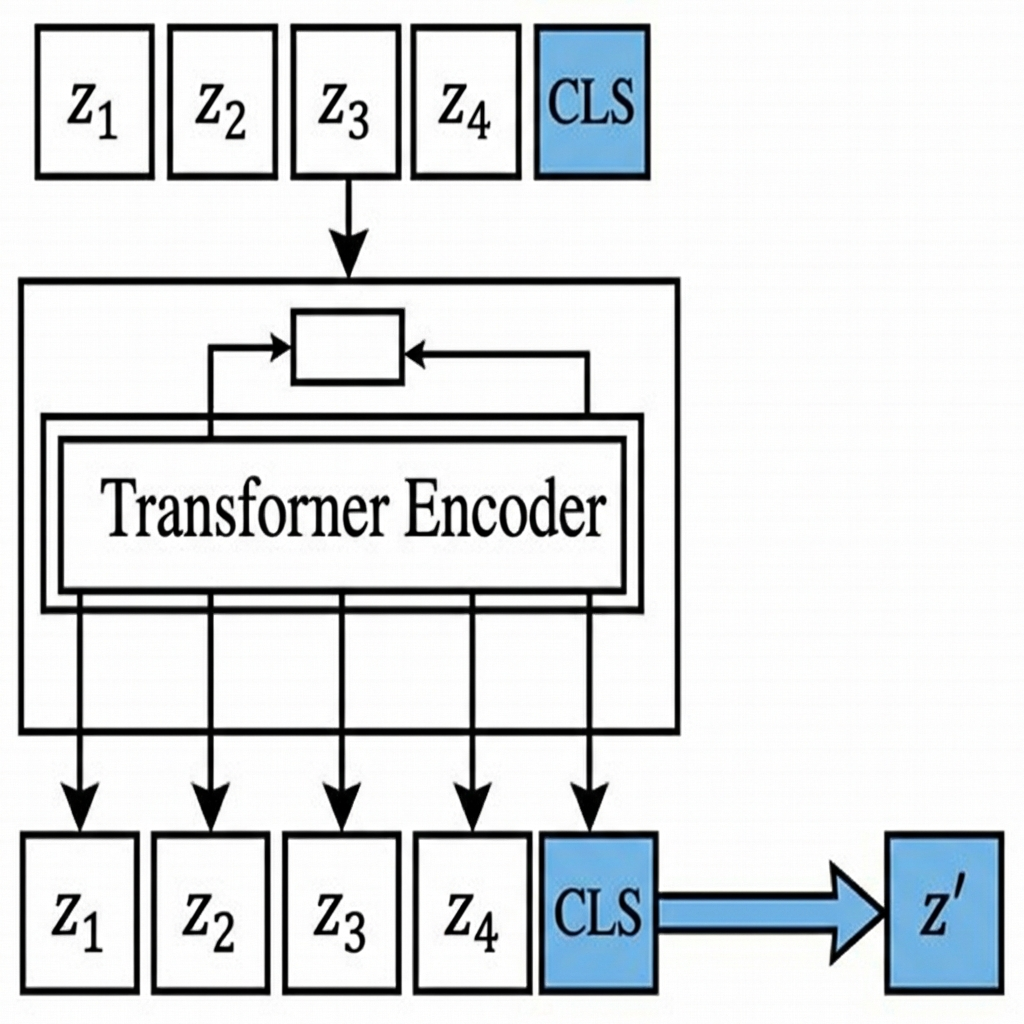
\includegraphics[width=0.9\linewidth]{images/local_cls_mechanism.png}
    \caption[مکانیزم توکن کلاس محلی]{نمای شماتیک از مکانیزم توکن کلاس محلی. توکن‌های داده در گروه‌های ۴تایی به همراه یک توکن کلاس یادگیرنده وارد بلوک پردازشی شده و تنها توکن کلاس به عنوان خروجی انتخاب می‌شود.}
    \label{fig:local_cls}
\end{figure}

فرآیند عملیاتی این روش شامل سه مرحله است. فرض کنید خروجی تعبیه‌ساز شاخه وضوح‌بالا با $Z_{x2} \in \mathbb{R}^{N \times 4T \times D}$ نمایش داده شود، که در آن $N$ اندازه دسته، $4T$ طول توالی شاخه \lr{x2} و $D$ بعد ویژگی است. در گام نخست، توکن‌ها بر اساس موقعیت مکانی به گروه‌های چهارتایی تقسیم می‌شوند:
\begin{equation}
    \label{eq:local-cls-grouping}
    Z_{\text{grouped}} = \text{Reshape}(Z_{x2}) \in \mathbb{R}^{N \times T \times 4 \times D}
\end{equation}
در این مرحله، $T$ گروه مجزا وجود دارد که هر گروه شامل چهار بردار ویژگی $z_{4i}, z_{4i+1}, z_{4i+2}, z_{4i+3}$ است.

در گام دوم، یک پارامتر قابل یادگیری اولیه $C_{init} \in \mathbb{R}^{1 \times 1 \times D}$ تعریف می‌شود و برای تمام گروه‌ها و تمام نمونه‌های دسته گسترش می‌یابد. سپس این توکن به انتهای هر گروه چهارتایی الحاق می‌شود و ورودی محلی پنج‌توکنی شکل می‌گیرد:
\begin{equation}
    \label{eq:local-cls-input}
    Z_{\text{input}}^{(i)} = \text{Concat}([z_{4i}, \dots, z_{4i+3}, c_{\text{token}}^{(i)}]) \in \mathbb{R}^{5 \times D}
\end{equation}
که در آن $Z_{\text{input}}^{(i)}$ ورودی مربوط به $i$-امین پنجره محلی است.

در گام سوم، گروه‌های پنج‌تایی به صورت توالی $N \times 5T \times D$ بازآرایی می‌شوند و از بلوک مبدل شاخه \lr{x2} عبور می‌کنند. در پیاده‌سازی نهایی، محلی بودن تجمیع از طریق گروه‌بندی چهارتایی و استخراج خروجی توکن کلاس هر گروه اعمال می‌شود؛ به بیان دیگر، پس از پردازش، فقط موقعیت‌های متناظر با توکن‌های کلاس نگه داشته می‌شوند:
\begin{equation}
    \label{eq:local-cls-transformer}
    Z_{\text{processed}} = \text{TransformerEncoder}(Z_{\text{flattened}})
\end{equation}
خروجی این تبدیل نیز دارای ابعاد $N \times 5T \times D$ است. وزن‌های بلوک مبدل و توکن کلاس محلی در طول آموزش تنظیم می‌شوند تا خروجی توکن کلاس بتواند بازنمایی فشرده‌ای از همان گروه محلی ایجاد کند.

در گام نهایی، از میان پنج خروجی مربوط به هر گروه، فقط بردار خروجی موقعیت توکن کلاس انتخاب می‌شود:
\begin{equation}
    \label{eq:local-cls-extraction}
    z'_{i} = Z_{\text{processed}}[i \times 5 + 4]
\end{equation}
(با فرض اینکه توکن کلاس در اندیس آخر، یعنی اندیس ۴ الحاق شده باشد).
بدین ترتیب، خروجی نهایی شاخه کمکی با $Z_{\text{cls}} \in \mathbb{R}^{N \times T \times D}$ نمایش داده می‌شود و از نظر طول توالی با خروجی بدنه اصلی سازگار است.

\subsection{مبدل بینایی به عنوان خبره (\lr{ViT as Expert})}
برای پردازش ویژگی‌های شاخه \lr{x2}، از یک بلوک مبدل برگرفته از مدل \lr{vit\_large\_patch16\_224} استفاده شده است. این بلوک با وزن‌های پیش‌آموزش‌دیده مقداردهی اولیه می‌شود تا شاخه کمکی از ابتدا دارای بازنمایی‌های بصری قابل استفاده باشد. از آنجا که بعد پنهان این مدل \lr{ViT} با بعد پنهان \lr{DiT-XL/2} یکسان نیست، پروجکشن‌های خطی ورودی و خروجی برای تبدیل ابعاد استفاده می‌شوند \cite{Dosovitskiy2020,5206848,2212.09748,wightman2019timm}.

\subsection{شرط‌گذاری اختیاری با \lr{FiLM}}
معماری \lr{DuoDiT} از نظر طراحی می‌تواند شاخه \lr{x2} را با مدولاسیون خطی ویژگی (\lr{FiLM}) به گام زمانی نویز و برچسب کلاس وابسته کند، اما این گزینه در آموزش اصلی \lr{ImageNet-1K} این پایان‌نامه فعال نشده است. بنابراین، نتایج فصل آزمایش‌ها بر اساس ویژگی‌های بدون مدولاسیون شاخه دوم گزارش می‌شوند و \lr{FiLM} به عنوان یک مسیر توسعه اختیاری برای تنظیمات شرطی پیچیده‌تر باقی می‌ماند \cite{perez2018film,2088740}.

در حالت فعال، بردار شرط $c = e_t + e_y$، که از ترکیب تعبیه زمان و تعبیه کلاس به دست می‌آید، به یک شبکه \lr{MLP} داده می‌شود تا ضرایب مقیاس و انتقال تولید شوند. این ضرایب پیش از ورود ویژگی‌های شاخه \lr{x2} به بلوک مبدل اعمال می‌شوند:
\begin{equation}
    \label{eq:film-conditioning}
    x_2' = \gamma(c) \cdot x_2 + \beta(c)
\end{equation}
\begin{figure}[H]
    \centering
    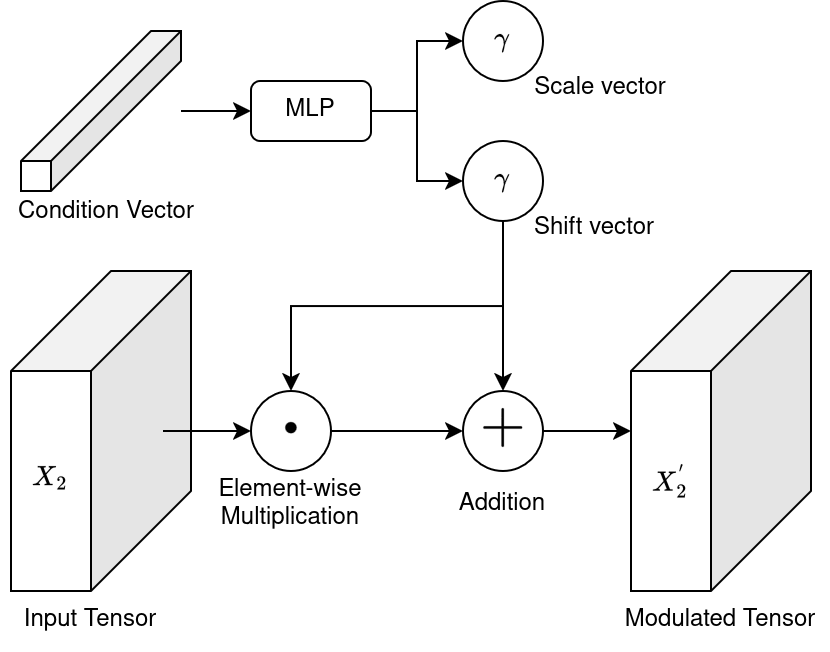
\includegraphics[width=0.9\linewidth]{images/film_modulation.png}
    \caption[بلوک شرط‌گذاری \lr{FiLM}]{بلوک شرط‌گذاری \lr{FiLM}. بردار شرط $c$ پارامترهای مقیاس و انتقال را تولید می‌کند که بر روی ورودی اعمال می‌شوند.}
    \label{fig:film_mod}
\end{figure}
سازوکار تولید و اعمال ضرایب مقیاس و انتقال در شکل \ref{fig:film_mod} نشان داده شده است. بررسی اثر فعال‌سازی این ماژول در رژیم‌های شرطی ریزدانه‌تر می‌تواند به عنوان یکی از مسیرهای آینده دنبال شود.

\subsection{ادغام نهایی}
پس از استخراج توکن‌های کلاس محلی، خروجی شاخه \lr{x2} از نظر طول توالی با خروجی بدنه اصلی هم‌اندازه است. در معماری نهایی این پژوهش، ادغام فقط در انتهای بدنه اصلی انجام می‌شود. اگر خروجی آخرین بلوک بدنه اصلی با $H_{\text{backbone}}^{(L)}$ و خروجی هم‌تراز شاخه کمکی با $H_{x2}$ نمایش داده شود، اتصال باقی‌مانده نهایی به صورت زیر است:
\begin{equation}
    \label{eq:dual-stream-fusion}
    H_{\text{fused}} = H_{\text{backbone}}^{(L)} + H_{x2}
\end{equation}
سپس 
$H_{\text{fused}}$
 وارد لایه نهایی 
 \lr{DiT}
 تا ویژگی‌های نهایی به دست آیند.
 
\section{استراتژی آموزش و تنظیم دقیق}
استراتژی آموزش \lr{DuoDiT} بر ثابت نگه داشتن بدنه اصلی و آموزش اجزای شاخه کمکی مبتنی است. هدف این طراحی، کاهش تعداد پارامترهای به‌روزرسانی‌شونده در عین حفظ امکان سازگارسازی بازنمایی‌های محلی است \cite{8409325,2212.09748}.

\subsection{مدیریت پارامترهای منجمد و آموزش‌پذیر}
در این روش، بدنه اصلی مدل انتشار (\lr{DiT Backbone}) که شامل لایه‌های تعبیه ورودی، بلوک‌های مبدل اصلی و لایه‌های مدولاسیون است، به طور کامل \textbf{منجمد (\lr{Frozen})} نگه داشته می‌شود. این کار باعث می‌شود دانش پیش‌آموزش‌دیده مدل پایه در طول تنظیم دقیق تغییر نکند \cite{8409325,2212.09748}.
در مقابل، اجزای زیر به عنوان پارامترهای قابل آموزش (\lr{Trainable Parameters}) فعال می‌شوند:
\begin{itemize}
    \item \textbf{تعبیه‌ساز پچ شاخه \lr{x2}}: برای یادگیری بازنمایی‌های اولیه با وضوح بالا.
    \item \textbf{توکن‌های کلاس محلی}: پارامترهای یادگیرنده‌ای که بازنمایی هر گروه محلی را خلاصه می‌کنند.
    \item \textbf{بلوک مبدل شاخه \lr{x2} و پروجکشن‌ها}: جهت پردازش عمیق ویژگی‌های جزئیات.
    \item \textbf{لایه خروجی (\lr{Final Layer})}: که امکان تطبیق نهایی خروجی مدل با فضای هدف را فراهم می‌کند.
\end{itemize}
این تفکیک پارامترها باعث می‌شود تنها \lr{17.95} میلیون پارامتر از مجموع \lr{690.39} میلیون پارامتر نیازمند ذخیره گرادیان و به‌روزرسانی باشند.

\subsection{مقداردهی اولیه با وزن‌های پیش‌آموزش‌دیده}
برای مقداردهی اولیه بلوک مبدل شاخه \lr{x2}، از وزن‌های پیش‌آموزش‌دیده مدل \lr{ViT-Large} آموزش‌دیده روی \lr{ImageNet} استفاده می‌شود. در صورتی که ابعاد فضای پنهان مدل \lr{DiT} با ابعاد مدل \lr{ViT} بارگذاری‌شده تفاوت داشته باشد، لایه‌های پروجکشن خطی برای تطبیق ابعاد اضافه و آموزش داده می‌شوند \cite{Dosovitskiy2020,5206848,wightman2019timm,2212.09748}.

\subsection{تثبیت آموزش با \lr{EMA}}
برای پایداری فرآیند آموزش و جلوگیری از نوسانات شدید در وزن‌ها، از روش میانگین متحرک نمایی\LTRfootnote{Exponential Moving Average} (\lr{EMA}) استفاده می‌شود. یک نسخه کپی از مدل که وزن‌های آن میانگین متحرک وزن‌های در حال آموزش است، نگهداری می‌شود و در نهایت برای تولید نمونه‌ها و ارزیابی کیفیت مورد استفاده قرار می‌گیرد \cite{2212.09748}.

\subsection{الگوریتم آموزش}
الگوریتم \ref{alg:training} روند آموزش \lr{DuoDiT} را به صورت گام‌به‌گام نشان می‌دهد. در این الگوریتم، بدنه اصلی \lr{DiT} ثابت است، شاخه \lr{x2} با توکن‌های کلاس محلی آموزش داده می‌شود، و ادغام دو جریان پس از آخرین بلوک بدنه اصلی انجام می‌گیرد.

برای پشتیبانی از \lr{CFG} در مرحله نمونه‌برداری، آموزش فقط به حالت شرطی محدود نمی‌شود. در هر تکرار، برچسب کلاس با احتمال $p_{\text{\lr{drop}}}$ با شرط تهی جایگزین می‌شود تا مدل واحد بتواند هر دو پیش‌بینی شرطی و بی‌شرط را یاد بگیرد. این کار تغییری در معماری \lr{DuoDiT} ایجاد نمی‌کند، اما در زمان نمونه‌برداری امکان ترکیب دو خروجی
$\epsilon_\theta(x_t,t,y)$
و
$\epsilon_\theta(x_t,t,\emptyset)$
را با ضریب \lr{CFG} فراهم می‌سازد \cite{ho2022classifierFreeGuidance}.

\begin{latin}
\begin{algorithm}[htbp]
\caption{Parameter-Efficient Training Loop for DuoDiT}
\label{alg:training}
\begin{algorithmic}[1]
\Require Pre-trained DiT Backbone $\theta_{\text{frozen}}$, Trainable x2-stream parameters $\phi$, Dataset $\mathcal{D}$, Learning Rate $\eta$, Label-drop probability $p_{\text{drop}}$
\State Initialize Second Stream Expert ViT block with pre-trained weights
\State Freeze all parameters in $\theta_{\text{frozen}}$
\While{not converged}
    \State Sample batch of images $x_0 \sim \mathcal{D}$ and class labels $y$
    \State With probability $p_{\text{drop}}$, replace $y$ with the null condition $\emptyset$
    \State Sample time steps $t \sim \text{Uniform}(1, T)$
    \State Sample noise $\epsilon \sim \mathcal{N}(0, I)$
    \State Compute noisy image $x_t = \sqrt{\bar{\alpha}_t}x_0 + \sqrt{1 - \bar{\alpha}_t}\epsilon$
    \State Extract final frozen-backbone features $h_{\text{backbone}}^{(L)} = \mathcal{F}(x_t, t, y; \theta_{\text{frozen}})$
    \State Extract high-resolution x2 tokens $h_{x2} = \mathcal{E}_{x2}(x_t; \phi_{\text{embed}})$
    \State Use (modulated) Second Stream features $h_{x2}' = h_{x2}$
    \State Group x2 tokens in sets of four and append local class tokens
    \State Process grouped sequence through Expert ViT block
    \State Extract local class-token positions and project them to DiT hidden dimension: $h_{\text{cls}}$
    \State Fuse after the final backbone block: $h_{\text{fused}} = h_{\text{backbone}}^{(L)} + h_{\text{cls}}$
    \State Predict noise $\epsilon_\theta = \text{FinalLayer}(h_{\text{fused}}; \phi_{\text{out}})$
    \State Compute Loss $\mathcal{L} = \| \epsilon - \epsilon_\theta \|^2$
    \State Update $\phi \gets \phi - \eta \nabla_\phi \mathcal{L}$
    \State Update EMA parameters $\phi_{\text{ema}} \gets 0.9999 \phi_{\text{ema}} + 0.0001 \phi$
\EndWhile
\end{algorithmic}
\end{algorithm}
\end{latin}

\subsection{کارایی پارامتری}
جدول \ref{tab:param_count} تحلیل کلان تعداد پارامترهای قابل آموزش در معماری \lr{DuoDiT} را نشان می‌دهد. با منجمد نگه‌داشتن بدنه اصلی \lr{DiT-XL/2} و آموزش فقط شاخه دوم، توکن‌های کلاس محلی، پروجکشن‌ها و لایه خروجی، تعداد پارامترهای آموزش‌پذیر به \lr{17.95} میلیون از \lr{690.39} میلیون پارامتر کل محدود می‌شود. این کاهش در تعداد وزن‌های به‌روزرسانی‌شونده، امکان اجرای تنظیم دقیق پارامتر-کارا را با هزینه حافظه و زمان کمتر فراهم می‌کند \cite{2212.09748,8409325}.

\begin{table}[htbp]
    \centering
    \caption[تحلیل پیچیدگی مدل]{تحلیل پیچیدگی مدل و تفکیک پارامترهای قابل آموزش}
    \label{tab:param_count}
    \begin{latin}
    \begin{tabular}{lrc}
        \hline
        \textbf{Component} & \textbf{Parameters (M)} & \textbf{Trainable} \\
        \hline
        Frozen DiT-XL/2 Backbone & 672.44 & False \\
        Trainable DuoDiT Components & 17.95 & True \\
        \hline
        \textbf{Total Parameters} & \textbf{690.39} & \\
        \hline
    \end{tabular}
    \end{latin}
\end{table}

\section{تابع هزینه}
فرض کنید $x_t$ نمونه نویزی در گام زمانی $t$ و $y$ برچسب کلاس باشد. بدنه اصلی منجمد با پارامترهای $\theta$ خروجی آخرین بلوک خود را به صورت زیر تولید می‌کند \cite{6206256,2212.09748}:
\begin{equation}
    \label{eq:backbone-final}
    H_{\text{backbone}}^{(L)} = \mathcal{F}_{\theta}(x_t, t, y), \quad
    H_{\text{backbone}}^{(L)} \in \mathbb{R}^{N \times T \times D}.
\end{equation}
شاخه \lr{x2} همان ورودی نویزی را با اندازه پچ کوچک‌تر پردازش می‌کند و توالی بلندتری به دست می‌دهد:
\begin{equation}
    \label{eq:x2-embed}
    Z_{x2} = \mathcal{E}_{x2}(x_t), \quad
    Z_{x2} \in \mathbb{R}^{N \times 4T \times D}.
\end{equation}
در آموزش اصلی این پژوهش، شاخه کمکی بدون مدولاسیون \lr{FiLM} وارد مرحله تجمیع می‌شود:
\begin{equation}
    \label{eq:x2-film}
    \tilde{Z}_{x2} = Z_{x2}.
\end{equation}
توکن‌های شاخه کمکی مطابق رابطه \ref{eq:local-cls-grouping} در گروه‌های چهارتایی قرار می‌گیرند، توکن کلاس محلی به هر گروه افزوده می‌شود و توالی حاصل از بلوک مبدل شاخه کمکی عبور می‌کند:
\begin{equation}
    \label{eq:x2-expert}
    U = \mathcal{T}_{\phi}(\text{Flatten}([\text{Group}(\tilde{Z}_{x2}); C])),
    \quad U \in \mathbb{R}^{N \times 5T \times D}.
\end{equation}
با انتخاب خروجی‌های متناظر با توکن‌های کلاس، توالی شاخه کمکی به طول $T$ کاهش می‌یابد:
\begin{equation}
    \label{eq:x2-cls-sequence}
    H_{x2} = \text{SelectClassToken}(U), \quad
    H_{x2} \in \mathbb{R}^{N \times T \times D}.
\end{equation}
در نهایت، خروجی شاخه کمکی پس از هم‌ترازسازی ابعاد، به خروجی آخرین بلوک بدنه اصلی افزوده می‌شود و لایه نهایی نویز را پیش‌بینی می‌کند:
\begin{equation}
    \label{eq:duodit-output}
    \epsilon_{\theta,\phi}(x_t,t,y) =
    \text{FinalLayer}_{\phi}(H_{\text{backbone}}^{(L)} + H_{x2}).
\end{equation}
تابع هزینه آموزشی همان خطای رایج پیش‌بینی نویز در مدل‌های انتشار است \cite{6206256,2212.09748}:
\begin{equation}
    \label{eq:duodit-loss}
    \mathcal{L}_{\text{DuoDiT}} =
    \mathbb{E}_{x_0,t,\epsilon,y}
    \left[
    \left\|
    \epsilon - \epsilon_{\theta,\phi}(x_t,t,y)
    \right\|_2^2
    \right].
\end{equation}
در این رابطه‌ها، $\theta$ ثابت است و فقط پارامترهای $\phi$، شامل تعبیه‌ساز شاخه \lr{x2}، توکن‌های کلاس محلی، بلوک مبدل شاخه کمکی، پروجکشن‌ها و لایه نهایی، به‌روزرسانی می‌شوند.

\section{جمع‌بندی}
در این فصل، معماری \lr{DuoDiT} برای تنظیم دقیق پارامتر-کارای مدل \lr{DiT} معرفی شد. روش نهایی شامل یک بدنه اصلی منجمد و یک شاخه وضوح‌بالا است که خروجی آن با مکانیزم توکن کلاس محلی از $4T$ توکن به $T$ توکن کاهش می‌یابد. سپس خروجی هم‌تراز شاخه کمکی پس از آخرین بلوک بدنه اصلی با جریان اصلی جمع شده و وارد لایه نهایی می‌شود. در این ساختار، راهبردهای ساده‌تری مانند پروجکشن خطی، بیشینه‌گیری و کمینه‌گیری به عنوان مبناهای مقایسه‌ای در نظر گرفته شده‌اند، اما معماری اصلی گزارش‌شده در این پایان‌نامه بر تجمیع مبتنی بر توکن کلاس محلی و ادغام نهایی \lr{x2\_final\_fuse} متکی است.

\chapter{آزمایش‌ها، نتایج و تحلیل}
\label{ch:experiments}

در این فصل، معماری \lr{DuoDiT} در سناریوی تولید تصویر شرطی روی \lr{ImageNet-1K} ارزیابی می‌شود. هدف اصلی، سنجش این پرسش است که آیا افزودن یک شاخه دوم با وضوح توکنی بالاتر، در حالی که بدنه اصلی \lr{DiT-XL/2} منجمد باقی می‌ماند، می‌تواند کیفیت توزیعی و ادراکی تولید را با بودجه پارامتری کوچک بهبود دهد یا خیر. به همین منظور، نتایج \lr{DuoDiT} با \lr{DiT-XL/2}، \lr{LightningDiT} و \lr{FineDiffusion} مقایسه می‌شود \cite{2212.09748,Yao2025LightningDiT,Pan2024FineDiffusion}.

\section{پیکربندی آزمایش}
ارزیابی اصلی بر روی تولید شرطی \lr{ImageNet-1K} در وضوح $256 \times 256$ انجام شده است \cite{5206848,imagenet15russakovsky}. مطابق پروتکل \lr{FID-50K}، تعداد ۵۰٬۰۰۰ تصویر تولید می‌شود؛ برچسب هر نمونه به‌صورت یکنواخت از میان ۱۰۰۰ کلاس 
\lr{ImageNet}
 انتخاب می‌گردد و سپس کیفیت نمونه‌ها در برابر آمار مرجع 
\lr{ImageNet}
 محاسبه می‌شود. 
\subsection{جزئیات پیاده‌سازی}
مدل پایه در تمام آزمایش‌ها \lr{DiT-XL/2} است که شامل ۲۸ بلوک مبدل، بعد پنهان ۱۱۵۲ و ۱۶ سر توجه است. شاخه اصلی با اندازه پچ ۲ روی فضای نهان عمل می‌کند، در حالی که شاخه دوم \lr{DuoDiT} اندازه پچ ۱ دارد و بنابراین توکن‌های ریزدانه‌تری تولید می‌کند. بلوک خبره \lr{ViT} در شاخه دوم از وزن‌های از پیش آموزش‌دیده \lr{vit\_large\_patch16\_224} مقداردهی اولیه شده و برای تطبیق بعد ۱۰۲۴ این بلوک با بعد ۱۱۵۲ در \lr{DiT-XL/2}، پروجکشن‌های خطی ورودی و خروجی آموزش داده می‌شوند \cite{Dosovitskiy2020,wightman2019timm,2212.09748}.

تصاویر ورودی با برش مرکزی، وارونگی تصادفی افقی و نرمال‌سازی به بازه $[-1,1]$ پیش‌پردازش می‌شوند. سپس تصاویر با استفاده از رمزگذار \lr{sd-vae-ft-ema} به فضای نهان $32 \times 32 \times 4$ نگاشت شده و ضریب مقیاس \lr{0.18215} اعمال می‌شود \cite{9851474}. بهینه‌ساز \lr{AdamW} با نرخ یادگیری ثابت $10^{-4}$، اندازه دسته سراسری ۲۵۶، ضرایب $\beta_1=0.9$ و $\beta_2=0.999$ و وزن‌کاهی صفر استفاده شده است \cite{loshchilov2019adamw}. مدل \lr{DuoDiT-200} برای ۲۰۰ دوره آموزش داده شده و نسخه \lr{DuoDiT-57} به‌عنوان نقطه میانی آموزش نیز گزارش می‌شود.

برای پایداری آموزش، میانگین متحرک نمایی (\lr{EMA}) با ضریب فروپاشی \lr{0.9999} روی وزن‌های آموزش‌پذیر اعمال شده است \cite{Polyak1992EMA,ho2020ddpm}. در نمونه‌برداری، از \lr{DDPM} با ۲۵۰ گام و ضریب هدایت بدون طبقه‌بند \lr{CFG=1.5} استفاده شده است \cite{ho2020ddpm,ho2022classifierFreeGuidance}. احتمال حذف برچسب کلاس در آموزش برابر \lr{0.1} است تا نمونه‌برداری شرطی و غیرشرطی برای \lr{CFG} پشتیبانی شود. به بیان عملی، این مقدار حذف برچسب باعث می‌شود همان مدل در زمان نمونه‌برداری بتواند هم خروجی وابسته به کلاس و هم خروجی مستقل از کلاس را تولید کند؛ سپس \lr{CFG} اختلاف این دو خروجی را تقویت می‌کند تا نمونه نهایی به برچسب انتخاب‌شده نزدیک‌تر شود. مقدار \lr{CFG=1.5} به‌عنوان تنظیم میانه استفاده شده است، زیرا هدف ارزیابی فقط تولید نمونه‌های بسیار کلاس‌محور نیست، بلکه حفظ تعادل میان وفاداری شرطی، تنوع و کیفیت توزیعی نیز اهمیت دارد.

\begin{table}[htbp]
    \centering
    \caption[خلاصه تنظیمات آموزش و نمونه‌برداری]{خلاصه ابرپارامترها و تنظیمات مورد استفاده در آموزش و نمونه‌برداری \lr{DuoDiT}.}
    \label{tab:hyperparams}
    \begin{latin}
    \resizebox{\textwidth}{!}{%
    \begin{tabular}{llc}
        \hline
        \textbf{Category} & \textbf{Parameter} & \textbf{Value} \\
        \hline
        \multirow{7}{*}{Model} & Architecture & DiT-XL/2 \\
         & Transformer Depth & 28 \\
         & Hidden Dimension & 1152 \\
         & Attention Heads & 16 \\
         & MLP Ratio & 4.0 \\
         & Main Patch Size & 2 \\
         & Second Stream Patch Size & 1 \\
        \hline
        \multirow{9}{*}{Training} & Image Resolution & $256 \times 256$ \\
         & VAE & sd-vae-ft-ema \\
         & Diffusion Steps & 1000 \\
         & Optimizer & AdamW \\
         & Learning Rate & $1 \times 10^{-4}$ \\
         & Global Batch Size & 256 \\
         & Epochs & 200 \\
         & Seed & 0 \\
         & Label Dropout & 0.1 \\
        \hline
        \multirow{2}{*}{Sampling} & DDPM Steps & 250 \\
         & CFG Scale & 1.5 \\
        \hline
    \end{tabular}%
    }
    \end{latin}
\end{table}

\section{نتایج کمی}
جدول \ref{tab:main_metrics} مقایسه اصلی مدل‌ها را نشان می‌دهد. \lr{LightningDiT} بهترین مقدار \lr{FID} گزارش‌شده را دارد، اما \lr{DuoDiT-200} در \lr{KID} و \lr{LPIPS-Mean} بهترین عملکرد را میان مدل‌های مقایسه‌شده ثبت می‌کند. این نتیجه نشان می‌دهد شاخه دوم \lr{DuoDiT} بیشتر از آنکه صرفاً یک تنظیم پارامتری سطحی باشد، می‌تواند در کیفیت ادراکی و شباهت توزیعی مبتنی بر \lr{KID} اثر بگذارد.

\begin{table}[htbp]
    \centering
    \caption[مقایسه کمی اصلی]{مقایسه کمی اصلی میان مدل‌های ارزیابی‌شده. معیارهای \lr{FID}، \lr{KID} و \lr{LPIPS-Mean} همگی کمتر-بهتر هستند.}
    \label{tab:main_metrics}
    \begin{latin}
    \footnotesize
    \resizebox{\textwidth}{!}{%
    \begin{tabular}{lcccc}
        \hline
        \textbf{Model} & \textbf{FID} ($\downarrow$) & \textbf{KID} ($\downarrow$) & \textbf{LPIPS-Mean} ($\downarrow$) & \textbf{Params/Trainable (M)} \\
        \hline
        DiT-XL/2 \cite{2212.09748} & 2.270$^\dagger$ & 0.0023 & 0.7209 & 675.00$^\dagger$ \\
        LightningDiT \cite{Yao2025LightningDiT} & \textbf{1.350}$^\dagger$ & 0.0016 & 0.7232 & 675.00$^\dagger$ \\
        FineDiffusion \cite{Pan2024FineDiffusion} & 9.674 & 0.0093 & 0.7802 & 685.64 / 12.15 \\
        \hline
        DuoDiT-57 & 4.95 & 0.0069 & 0.7175 & 690.39 / 17.95 \\
        DuoDiT-200 & 2.219 & \textbf{0.0014} & \textbf{0.7162} & 690.39 / 17.95 \\
        \hline
    \end{tabular}%
    }
    \end{latin}
    \begin{minipage}{0.96\linewidth}
        \footnotesize
        مقادیر دارای $^\dagger$ از گزارش رسمی مقاله یا پروژه متناظر گرفته شده‌اند. \lr{DuoDiT-57} و \lr{DuoDiT-200} معماری یکسان دارند و تفاوت آن‌ها در تعداد دوره‌های آموزش است.
    \end{minipage}
\end{table}

جدول \ref{tab:classwise_fid_aggregate} آمار تجمعی \lr{FID} کلاسی را نشان می‌دهد. میانگین کلاسی \lr{DuoDiT-57} کمی بهتر از سایر مدل‌هاست، در حالی که \lr{DuoDiT-200} کمترین انحراف معیار را ثبت می‌کند. این الگو نشان می‌دهد افزایش تعداد دوره‌های آموزش، علاوه بر بهبود معیارهای اصلی، پراکندگی عملکرد کلاسی را نیز پایدارتر می‌کند.

\begin{table}[htbp]
    \centering
    \caption[آمار تجمعی \lr{FID} کلاسی]{آمار تجمعی \lr{FID} کلاسی روی کلاس‌های ارزیابی‌شده \lr{ImageNet}.}
    \label{tab:classwise_fid_aggregate}
    \begin{latin}
    \footnotesize
    \resizebox{\textwidth}{!}{%
    \begin{tabular}{lccc}
        \hline
        \textbf{Model} & \textbf{Mean} & \textbf{Std.} & \textbf{Range} \\
        \hline
        DiT & 109.4829 & 46.6011 & 27.3300--254.8514 \\
        LightningDiT & 110.6087 & 46.2643 & 28.8194--254.1752 \\
        FineDiffusion & 306.0911 & 67.4299 & 69.0698--807.0562 \\
        \hline
        DuoDiT-57 & \textbf{108.5531} & 46.3826 & 26.7390--278.0763 \\
        DuoDiT-200 & 109.5321 & \textbf{46.1673} & 27.4746--253.7685 \\
        \hline
    \end{tabular}%
    }
    \end{latin}
\end{table}

\section{نتایج کیفی}
شکل \ref{fig:duodit_visual_results} نمونه‌هایی از خروجی‌های \lr{DuoDiT-200} را برای کلاس‌های مختلف نشان می‌دهد.
\begin{figure}[H]
    \centering
    \begin{minipage}[t]{0.225\textwidth}
        \centering
        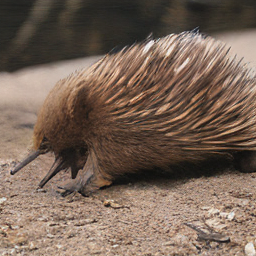
\includegraphics[width=\linewidth]{images/028102-class0102.png}
    \end{minipage}\hspace{0.01\textwidth}
    \begin{minipage}[t]{0.225\textwidth}
        \centering
        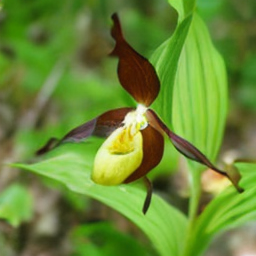
\includegraphics[width=\linewidth]{images/009986-class0986.png}
    \end{minipage}\hspace{0.01\textwidth}
    \begin{minipage}[t]{0.225\textwidth}
        \centering
        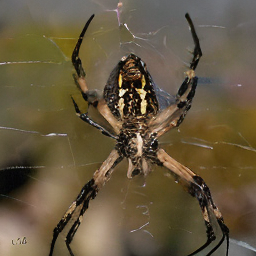
\includegraphics[width=\linewidth]{images/028072-class0072.png}
    \end{minipage}\hspace{0.01\textwidth}
    \begin{minipage}[t]{0.225\textwidth}
        \centering
        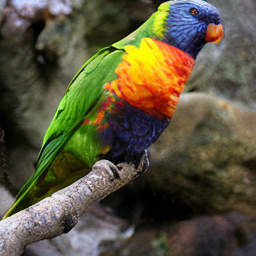
\includegraphics[width=\linewidth]{images/023090-class0090.png}
    \end{minipage}

    \vspace{1mm}

    \begin{minipage}[t]{0.225\textwidth}
        \centering
        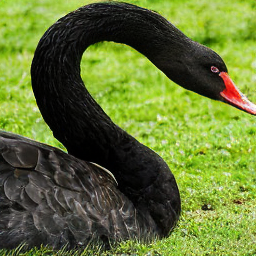
\includegraphics[width=\linewidth]{images/044100-class0100.png}
    \end{minipage}\hspace{0.01\textwidth}
    \begin{minipage}[t]{0.225\textwidth}
        \centering
        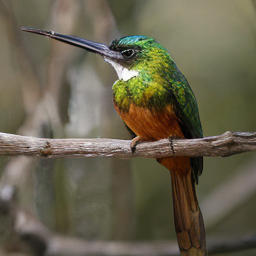
\includegraphics[width=\linewidth]{images/037095-class0095.png}
    \end{minipage}\hspace{0.01\textwidth}
    \begin{minipage}[t]{0.225\textwidth}
        \centering
        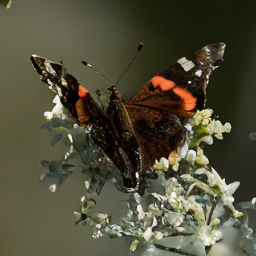
\includegraphics[width=\linewidth]{images/007321-class0321.png}
    \end{minipage}\hspace{0.01\textwidth}
    \begin{minipage}[t]{0.225\textwidth}
        \centering
        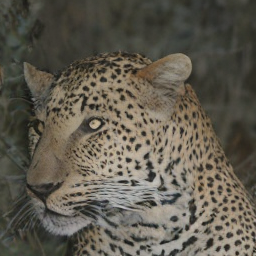
\includegraphics[width=\linewidth]{images/043288-class0288.png}
    \end{minipage}

    \vspace{1mm}

    \begin{minipage}[t]{0.225\textwidth}
        \centering
        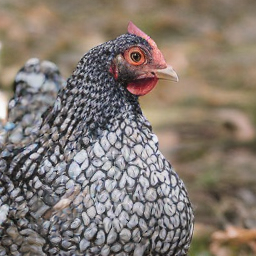
\includegraphics[width=\linewidth]{images/013008-class0008.png}
    \end{minipage}\hspace{0.01\textwidth}
    \begin{minipage}[t]{0.225\textwidth}
        \centering
        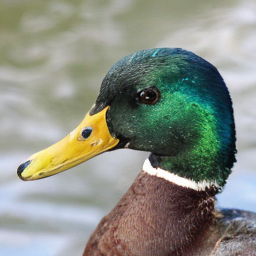
\includegraphics[width=\linewidth]{images/021097-class0097.png}
    \end{minipage}\hspace{0.01\textwidth}
    \begin{minipage}[t]{0.225\textwidth}
        \centering
        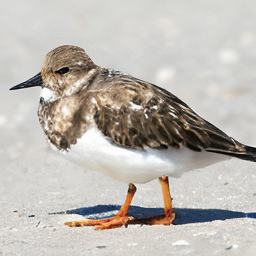
\includegraphics[width=\linewidth]{images/015139-class0139.png}
    \end{minipage}\hspace{0.01\textwidth}
    \begin{minipage}[t]{0.225\textwidth}
        \centering
        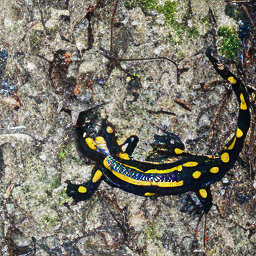
\includegraphics[width=\linewidth]{images/024025-class0025.png}
    \end{minipage}

    \vspace{1mm}

    \begin{minipage}[t]{0.225\textwidth}
        \centering
        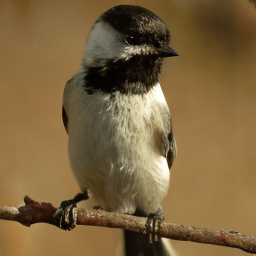
\includegraphics[width=\linewidth]{images/047019-class0019.png}
    \end{minipage}\hspace{0.01\textwidth}
    \begin{minipage}[t]{0.225\textwidth}
        \centering
        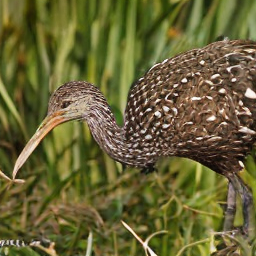
\includegraphics[width=\linewidth]{images/005135-class0135.png}
    \end{minipage}\hspace{0.01\textwidth}
    \begin{minipage}[t]{0.225\textwidth}
        \centering
        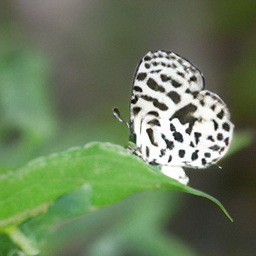
\includegraphics[width=\linewidth]{images/023326-class0326.png}
    \end{minipage}\hspace{0.01\textwidth}
    \begin{minipage}[t]{0.225\textwidth}
        \centering
        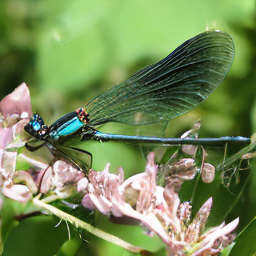
\includegraphics[width=\linewidth]{images/039320-class0320.png}
    \end{minipage}

    \vspace{1mm}

    \begin{minipage}[t]{0.225\textwidth}
        \centering
        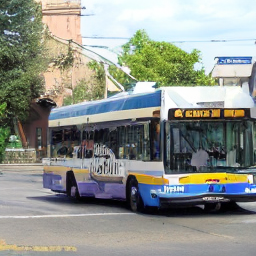
\includegraphics[width=\linewidth]{images/030874-class0874.png}
    \end{minipage}\hspace{0.01\textwidth}
    \begin{minipage}[t]{0.225\textwidth}
        \centering
        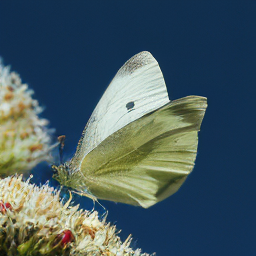
\includegraphics[width=\linewidth]{images/000324-class0324.png}
    \end{minipage}\hspace{0.01\textwidth}
    \begin{minipage}[t]{0.225\textwidth}
        \centering
        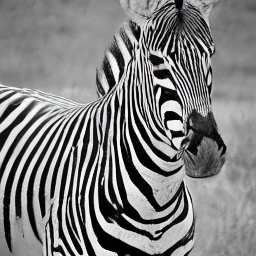
\includegraphics[width=\linewidth]{images/026340-class0340.png}
    \end{minipage}\hspace{0.01\textwidth}
    \begin{minipage}[t]{0.225\textwidth}
        \centering
        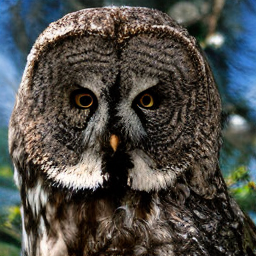
\includegraphics[width=\linewidth]{images/010024-class0024.png}
    \end{minipage}
    \caption[نمونه‌های تصویری \lr{DuoDiT-200}]{نمونه‌های تصویری تولیدشده توسط \lr{DuoDiT-200} روی کلاس‌های مختلف \lr{ImageNet}.}
    \label{fig:duodit_visual_results}
\end{figure}

\section{مطالعه انسانی}
برای تکمیل معیارهای خودکار، یک مطالعه انسانی میان نمونه‌های \lr{DuoDiT} و \lr{LightningDiT} انجام شده است. این مطالعه روی کلاس‌هایی از \lr{Mini-ImageNet}، به عنوان زیرمجموعه‌ای فشرده از \lr{ImageNet}، اجرا شده و شامل ۱۳ شرکت‌کننده است \cite{imagenet15russakovsky}. هر شرکت‌کننده ۳۰۰ مقایسه زوجی انجام داده و در مجموع ۳۹۰۰ پاسخ ثبت شده است.

\begin{table}[htbp]
    \centering
    \caption[نتایج مطالعه ترجیح انسانی]{نتایج مطالعه ترجیح انسانی برای مقایسه نمونه‌های \lr{DuoDiT} و \lr{LightningDiT}.}
    \label{tab:user_study_results}
    \begin{latin}
    \footnotesize
    \resizebox{\textwidth}{!}{%
    \begin{tabular}{ccccc}
        \hline
        \textbf{DuoDiT} & \textbf{LightningDiT} & \textbf{Tie} & \textbf{Total} & \textbf{DuoDiT Pref.} \\
        \hline
        1593 (40.85\%) & 1398 (35.85\%) & 909 (23.31\%) & 3900 & 53.26\% \\
        \hline
    \end{tabular}%
    }
    \end{latin}
    \begin{minipage}{0.96\linewidth}
        \footnotesize
        مقدار \lr{DuoDiT Pref.} از مقایسه‌های غیرمساوی محاسبه شده است؛ یعنی نسبت انتخاب‌های \lr{DuoDiT} به مجموع انتخاب‌های \lr{DuoDiT} و \lr{LightningDiT}.
    \end{minipage}
\end{table}

نتایج جدول \ref{tab:user_study_results} نشان می‌دهد با وجود برتری \lr{LightningDiT} در \lr{FID} کلی، نمونه‌های \lr{DuoDiT} در قضاوت انسانی سهم بیشتری از انتخاب‌های غیرمساوی را به دست آورده‌اند. این اختلاف با نتیجه \lr{LPIPS-Mean} همسو است و نشان می‌دهد شاخه وضوح‌بالا می‌تواند روی ویژگی‌هایی اثر بگذارد که در ادراک انسانی مهم هستند.

\section{هزینه محاسباتی و کارایی پارامتری}
جدول \ref{tab:compute_finediffusion} هزینه محاسباتی \lr{DuoDiT-200} را با \lr{FineDiffusion} مقایسه می‌کند. \lr{FineDiffusion} تعداد پارامتر آموزش‌پذیر کمتری دارد، اما در تنظیم پروفایل‌شده زمان هر دوره و مصرف حافظه بیشتری ثبت کرده است. در مقابل، \lr{DuoDiT-200} با \lr{17.95M} پارامتر آموزش‌پذیر، زمان هر دوره \lr{13m} و مصرف حافظه اوج \lr{2.91GB} را نشان می‌دهد.

\begin{table}[htbp]
    \centering
    \caption[مقایسه هزینه محاسباتی]{مقایسه هزینه محاسباتی و حافظه‌ای \lr{DuoDiT} و \lr{FineDiffusion} در تولید $256 \times 256$ \cite{Pan2024FineDiffusion}.}
    \label{tab:compute_finediffusion}
    \begin{latin}
    \footnotesize
    \resizebox{\textwidth}{!}{%
    \begin{tabular}{lccccc}
        \hline
        \textbf{Method} & \textbf{GFLOPs} & \textbf{Params} & \textbf{Trainable} & \textbf{Time/Epoch} & \textbf{VRAM} \\
        \hline
        DuoDiT-200 & 267.10 & 690.39M & 17.95M & 13m & 2.91GB \\
        FineDiffusion & 228.84 & 685.64M & 12.15M & 22m & 3.19GB \\
        \hline
    \end{tabular}%
    }
    \end{latin}
\end{table}

\section{مطالعات حذفی}
مطالعات حذفی برای جدا کردن اثر انتخاب‌های معماری انجام شده‌اند. این بخش شامل نتایج مربوط به راهبردهای تجمیع ویژگی، عمق شاخه دوم و نقش استفاده از ویژگی‌های \lr{ViT} و ضریب \lr{CFG} است. نتایج تجمیع ویژگی در سناریوی کنترل‌شده پنج‌کلاس ۹۷۲ تا ۹۷۶ گزارش شده‌اند تا اثر مکانیزم توکن کلاس محلی به‌صورت مستقیم با روش‌های ساده‌تر مقایسه شود.

\subsection{راهبردهای تجمیع ویژگی}
جدول \ref{tab:ablation_pooling} نشان می‌دهد که توکن کلاس محلی در مقایسه با میانگین‌گیری، بیشینه‌گیری و پروجکشن خطی بهترین مقدار را در هر سه معیار به دست می‌آورد. این نتیجه با انگیزه معماری سازگار است: تجمیع ثابت، همه نواحی مکانی را با قاعده یکسان خلاصه می‌کند، در حالی که توکن کلاس محلی از مکانیزم خود توجه برای استخراج محتوا-آگاه اطلاعات هر گروه چهار توکنی استفاده می‌کند.

\begin{table}[htbp]
    \centering
    \caption[مطالعه حذفی راهبردهای تجمیع]{مطالعه حذفی راهبردهای تجمیع برای هم‌تراز کردن توکن‌های شاخه دوم با شبکه توکنی \lr{DiT}.}
    \label{tab:ablation_pooling}
    \begin{latin}
    \begin{tabular}{lccc}
        \hline
        \textbf{Strategy} & \textbf{FID} ($\downarrow$) & \textbf{KID} ($\downarrow$) & \textbf{LPIPS-Mean} ($\downarrow$) \\
        \hline
        Average Pooling & 142.31 & 0.0452 & 0.7489 \\
        Max Pooling & 140.85 & 0.0438 & 0.7412 \\
        Linear Projection & 138.92 & 0.0415 & 0.7352 \\
        Local CLS Token & \textbf{135.78} & \textbf{0.0396} & \textbf{0.7018} \\
        \hline
    \end{tabular}
    \end{latin}
\end{table}

\subsection{عمق شاخه دوم}
جدول \ref{tab:ablation_blocks} هزینه اضافه کردن بلوک‌های بیشتر در شاخه دوم را نشان می‌دهد. افزایش عمق از یک بلوک به دو و چهار بلوک، \lr{GFLOPs}، زمان هر دوره و مصرف حافظه را افزایش می‌دهد. بنابراین تنظیم یک بلوک، نقطه تعادل مناسبی میان ظرفیت محلی و هزینه محاسباتی فراهم می‌کند.

\begin{table}[htbp]
    \centering
    \caption[مطالعه حذفی عمق شاخه دوم]{مطالعه حذفی عمق شاخه دوم از نظر محاسبات، زمان و حافظه.}
    \label{tab:ablation_blocks}
    \begin{latin}
    \begin{tabular}{lccc}
        \hline
        \textbf{Variant} & \textbf{GFLOPs} & \textbf{Time/Epoch} & \textbf{VRAM} \\
        \hline
        1 block & 267.10 & 13mins & 2.91GB \\
        2 blocks & 299.32 & 15mins & 2.99GB \\
        4 blocks & 363.75 & 26mins & 3.15GB \\
        \hline
    \end{tabular}
    \end{latin}
\end{table}

\subsection{ویژگی‌های شاخه دوم و ضریب \lr{CFG}}
جدول \ref{tab:ablation_vit} دو نوع تحلیل را نشان می‌دهد. در بخش نخست، استفاده از ویژگی‌های بلوک \lr{ViT} نسبت به اتصال ساده عملکرد کمی بهتری ثبت می‌کند. در بخش دوم، اثر ضریب \lr{CFG} بررسی شده است. باید توجه داشت که \lr{CFG} بخشی از معماری آموزش‌پذیر \lr{DuoDiT} نیست، بلکه ابرپارامتر مرحله نمونه‌برداری است؛ بنابراین تغییر آن مسیر حذف نویز و شدت شرط‌گذاری را تغییر می‌دهد، اما تعداد پارامترها یا ساختار شاخه دوم را عوض نمی‌کند.

در این تنظیم حذفی، ضریب \lr{CFG=1.0} بهترین \lr{FID} و \lr{KID} را دارد. افزایش ضریب به \lr{2.0} مقدار \lr{FID} را از \lr{210.3986} به \lr{215.7946} و مقدار \lr{KID} را از \lr{0.04142} به \lr{0.05030} افزایش می‌دهد. افزایش بیشتر ضریب به \lr{4.0} افت شدیدتری ایجاد می‌کند و \lr{FID} به \lr{230.0816} و \lr{KID} به \lr{0.06270} می‌رسد. این الگو نشان می‌دهد در این آزمایش، تقویت بیش از حد شرط باعث دور شدن نمونه‌ها از توزیع مرجع می‌شود. با این حال، تنظیم نهایی پایان‌نامه برای ارزیابی اصلی از \lr{CFG=1.5} استفاده می‌کند تا میان وفاداری شرطی و تنوع نمونه‌ها تعادل حفظ شود.

\begin{table}[htbp]
    \centering
    \caption[مطالعه حذفی شاخه دوم و \lr{CFG}]{مطالعه حذفی استفاده از ویژگی‌های شاخه دوم و مقدار ضریب \lr{CFG}.}
    \label{tab:ablation_vit}
    \begin{latin}
    \begin{tabular}{lcc}
        \hline
        \textbf{Variant} & \textbf{FID} ($\downarrow$) & \textbf{KID} ($\downarrow$) \\
        \hline
        Skip Connection & 216.7914 & 0.0512 \\
        ViT block features & 215.7946 & 0.0503 \\
        \hline
        CFG = 1.0 & 210.3986 & 0.04142 \\
        CFG = 2.0 & 215.7946 & 0.05030 \\
        CFG = 4.0 & 230.0816 & 0.06270 \\
        \hline
    \end{tabular}
    \end{latin}
\end{table}

تفسیر این نتیجه با نقش نظری \lr{CFG} سازگار است. ضریب بزرگ‌تر معمولاً نمونه‌ها را از نظر معنایی به کلاس خواسته‌شده نزدیک‌تر می‌کند و می‌تواند برای ارزیابی انسانی یا تولید نمونه‌های واضح‌تر مفید باشد، اما همین تقویت ممکن است تنوع درون‌کلاسی را کم کند. معیارهایی مانند \lr{FID} و \lr{KID} فقط وضوح یا تشخیص‌پذیری کلاس را اندازه نمی‌گیرند، بلکه شباهت توزیع تصاویر تولیدی به توزیع واقعی را نیز می‌سنجند. بنابراین، اگر \lr{CFG} خیلی زیاد باشد، خروجی‌ها ممکن است از نظر شرطی قوی‌تر اما از نظر توزیعی کم‌تنوع‌تر شوند و امتیاز بدتری بگیرند. به همین دلیل، در تحلیل نتایج این پایان‌نامه، \lr{CFG} به‌عنوان عامل کنترل‌کننده نمونه‌برداری از اثر معماری شاخه دوم جدا تفسیر می‌شود.

\section{بحث}
نتایج این فصل نشان می‌دهد \lr{DuoDiT} یک مسیر مکمل برای تنظیم دقیق پارامتر-کارای \lr{DiT} فراهم می‌کند. بدنه منجمد \lr{DiT} ساختار معنایی و دانش تولیدی پیش‌آموزش‌دیده را حفظ می‌کند، در حالی که شاخه دوم با اندازه پچ کوچک‌تر ویژگی‌های محلی بیشتری را در اختیار مدل قرار می‌دهد. مکانیزم توکن کلاس محلی نیز این ویژگی‌های ریزدانه را بدون افزایش طول توالی بدنه اصلی، به شبکه توکنی \lr{DiT} منتقل می‌کند.

برتری \lr{DuoDiT-200} در \lr{KID} و \lr{LPIPS-Mean} نشان می‌دهد اثر شاخه دوم بیشتر در شباهت توزیعی پایدار و کیفیت ادراکی ظاهر می‌شود. از سوی دیگر، مقدار \lr{FID} مدل همچنان از \lr{LightningDiT} بالاتر است؛ بنابراین ادعای این پایان‌نامه جایگزینی کامل روش‌های آموزش بزرگ‌مقیاس نیست، بلکه ارائه یک مسیر سبک برای تقویت مدل منجمد است. محدودیت اصلی آن است که شاخه محلی در برخی نمونه‌های دارای مرزهای مبهم یا بافت‌های بسیار متراکم ممکن است ساختار محلی نادرست را نیز تقویت کند. بررسی شرط‌گذاری اختیاری \lr{FiLM} و طراحی چندمقیاسی شاخه دوم می‌تواند در پژوهش‌های آینده برای کاهش این خطاها مطالعه شود.


\chapter{نتیجه‌گیری و پیشنهادها}
\label{ch:conclusion}

\section{خلاصه و دستاوردها}
در این پژوهش، معماری \lr{DuoDiT} به عنوان یک رویکرد دوجریانی برای تنظیم دقیق پارامتر-کارای مدل‌های انتشار مبتنی بر مبدل معرفی شد. هسته اصلی روش، حفظ بدنه پیش‌آموزش‌دیده \lr{DiT-XL/2} به صورت منجمد و افزودن یک شاخه دوم سبک با وضوح توکنی بالاتر است. این شاخه از طریق توکن‌های کلاس محلی با جریان اصلی هم‌تراز می‌شود و بدون آموزش مجدد کامل بدنه، امکان تزریق ویژگی‌های محلی و ریزدانه را فراهم می‌کند \cite{2212.09748,8409325}.

مهم‌ترین دستاوردهای این پژوهش عبارتند از:
\begin{enumerate}
    \item \textbf{معماری دوجریانی \lr{DuoDiT}}: طراحی یک شاخه دوم با اندازه پچ کوچک‌تر که در کنار بدنه اصلی منجمد عمل می‌کند و ویژگی‌های محلی را پیش از ادغام با جریان اصلی استخراج می‌نماید.
    \item \textbf{مکانیزم توکن کلاس محلی}: یک راهبرد محتوا-آگاه برای تجمیع ویژگی‌های شاخه دوم که در مطالعه حذفی نسبت به میانگین‌گیری، بیشینه‌گیری و پروجکشن خطی عملکرد بهتری ثبت کرده است.
    \item \textbf{ارزیابی بزرگ‌مقیاس}: ارزیابی روی \lr{ImageNet-1K} نشان داد که \lr{DuoDiT-200} با \lr{17.95M} پارامتر آموزش‌پذیر از مجموع \lr{690.39M} پارامتر، به \lr{FID=2.219}، \lr{KID=0.0014} و \lr{LPIPS-Mean=0.7162} می‌رسد \cite{heusel2017fid,binkowski2018kid,zhang2018lpips}.
    \item \textbf{شواهد ادراکی انسانی}: در مطالعه ترجیح انسانی میان \lr{DuoDiT} و \lr{LightningDiT}، مدل پیشنهادی در \lr{53.26\%} مقایسه‌های غیرمساوی ترجیح داده شد، که با بهبود \lr{LPIPS-Mean} همسو است \cite{Yao2025LightningDiT}.
\end{enumerate}

\section{پیشنهادهایی برای پژوهش‌های آینده}
بر اساس یافته‌های این پژوهش، مسیرهای زیر برای تحقیقات آتی پیشنهاد می‌شود:
\begin{enumerate}
    \item \textbf{بررسی شرط‌گذاری اختیاری \lr{FiLM}}: فعال‌سازی و ارزیابی کنترل‌شده \lr{FiLM} در تنظیمات شرطی ریزدانه‌تر می‌تواند نشان دهد آیا همگام‌سازی مستقیم شاخه دوم با زمان و کلاس بهبود معناداری ایجاد می‌کند یا خیر \cite{perez2018film}.
    \item \textbf{شاخه‌های کمکی چندمقیاسی}: توسعه بیش از یک شاخه وضوح‌بالا می‌تواند به مدل اجازه دهد جزئیات محلی را در چند مقیاس مکانی همزمان پردازش کند.
    \item \textbf{کاهش هزینه استنتاج}: ترکیب \lr{DuoDiT} با روش‌هایی مانند کوانتیزاسیون پس از آموزش یا مسیرهای محاسباتی پویا می‌تواند هزینه اجرای مدل را کاهش دهد \cite{2406.17343}.
    \item \textbf{تعمیم به تولید متن-به-تصویر و ویدئو}: استفاده از شاخه دوم در مدل‌های شرطی متنی یا ویدئویی می‌تواند نشان دهد آیا این ایده فراتر از تولید کلاسی \lr{ImageNet} نیز مفید است یا خیر \cite{9851474,8313484}.
    \item \textbf{جایگزینی بدنه اصلی/خبره}: جایگزینی اجزای اصلی مدل، مانند بدنه اصلی یا خبره، با مدل‌های دیگر می‌تواند منجر به بهبود عملکرد و کاهش هزینه محاسباتی شود.
\end{enumerate}

در مجموع، \lr{DuoDiT} نشان می‌دهد که اصلاحات معماری هدفمند می‌توانند مسیر مؤثری برای تنظیم دقیق پارامتر-کارای مدل‌های انتشار مبتنی بر مبدل باشند. این روش جایگزین آموزش بزرگ‌مقیاس مدل‌های قدرتمندتر نیست، بلکه راهکاری برای بهره‌گیری از دانش یک بدنه منجمد و افزودن ظرفیت محلی با هزینه محدود فراهم می‌کند.

%\lhead{}

\pagestyle{fancy}
\fancyhf{}
\fancyhead[RE]{\rightmark}
\fancyhead[LO]{\leftmark}
\fancyhead[LE,RO]{\thepage}

%\renewcommand{\bibname}{کتاب‌نامه}

\setLTRbibitems
%\begin{thebibliography}{99}
%\resetlatinfont
%\persian
%\latin
%\renewcommand{\bibname}{کتاب‌نامه}
%\bibliography{references.bib}
%\bibliographystyle{ieeetr}
%\end{thebibliography}

\cfoot{}
\lhead{کتاب‌نامه}
%\lr{
\bibliographystyle{plain}
\bibliography{references}
%}
}
% \appendix
% \chapter{‌متن برنامه‌ها}
\thispagestyle{empty}
در این پیوست، بخش‌های کلیدی از پیاده‌سازی معماری \lr{x2-DiT} ارائه شده است. تمرکز اصلی بر روی متد \lr{forward} است که در آن جریان ورودی با وضوح بالا (\lr{x2}) پردازش شده و توکن‌های کلاس محلی برای تجمیع ویژگی‌ها در آن درج می‌شوند. این کد نشان می‌دهد که چگونه دو جریان داده به‌صورت همزمان مدیریت می‌شوند.

\begin{latin}
\begin{python}
def forward(self, x, t, y):
    """
    Forward pass of x2-DiT.
    x: (N, C, H, W) tensor of spatial inputs
    t: (N,) tensor of diffusion timesteps
    y: (N,) tensor of class labels
    """

    # 1. Process high-resolution stream (x2)
    x2 = self.x2_embedder(x)  # (N, 4T, D)

    # Insert class tokens after every 4 patches to create local groups
    N, seq_len, D = x2.shape
    T = seq_len // 4

    # Reshape to group patches: (N, 4T, D) -> (N, T, 4, D)
    x2 = x2.reshape(N, T, 4, D)

    # Expand learnable class tokens: (1, T, D) -> (N, T, 1, D)
    x2_cls_tokens_expanded = self.x2_cls_tokens.repeat(N, 1, 1).unsqueeze(2)

    # Concatenate class tokens: (N, T, 4, D) + (N, T, 1, D) -> (N, T, 5, D)
    x2 = torch.cat([x2, x2_cls_tokens_expanded], dim=2)

    # Reshape back to sequence: (N, 5T, D)
    x2 = x2.reshape(N, 5 * T, D)

    # 2. Process main stream (standard DiT)
    x = self.x_embedder(x) + self.pos_embed  # (N, T, D)
    t = self.t_embedder(t)                   # (N, D)
    y = self.y_embedder(y, self.training)    # (N, D)
    c = t + y                                # (N, D)

    # The rest of the forward pass continues with block processing...
    # ...
\end{python}
\end{latin}

در کد فوق، مشاهده می‌شود که چگونه یک توکن کلاس یادگیرنده به ازای هر گروه ۴ تایی از پچ‌های \lr{x2} اضافه می‌شود. این ساختار به مدل اجازه می‌دهد تا اطلاعات محلی را به‌طور موثرتری نسبت به روش‌های سنتی مانند عملیات تجمیع و کاهش طول توالی ویژگی‌ها (\lr{Pooling}) جذب و نمایندگی کند.

{\baselineskip=.75cm
%\include{namname}
%\include{dicfa2en}
%\include{dicen2fa}
\printindex
% در این فایل، عنوان پایان‌نامه، مشخصات خود و چکیده پایان‌نامه را به انگلیسی، وارد کنید.
% توجه داشته باشید که جدول حاوی مشخصات پایان‌نامه/رساله، به طور خودکار، رسم می‌شود.
%%%%%%%%%%%%%%%%%%%%%%%%%%%%%%%%%%%%
\baselineskip=.6cm
\begin{latin}
    \latinfaculty{Faculty of Mathematical Sciences}
    \latindegree{Master of Computer Science}
    \latinuniversity{Tarbiat Modares University}
% group
\latinsubject{Department of Computer Science}
\latinfield{Specialization in Data Mining}
\latintitle{Improving Diffusion Models Based on Vision Transformers for Image Generation}
\firstlatinsupervisor{Dr.\ Mansoor Rezghi Ahaq}
%\secondlatinsupervisor{Second Supervisor}
%\firstlatinadvisor{First Advisor}
%\secondlatinadvisor{Second Advisor}
\latinname{Mostafa}
\latinsurname{Shahbazi Dil}
\latinthesisdate{2026 Feb}
\latinkeywords{Vision transformers, diffusion models, local and global features, feature aggregation, parameter-efficient fine-tuning}
\newpage
\thispagestyle{empty}
\baselineskip=.750cm
\en-abstract{%\noindent
Diffusion transformer models, such as DiT, provide high quality in class-conditional image generation, but fully fine-tuning them for new domains or requirements is costly in terms of memory, training time, and storage. This thesis introduces DuoDiT as a parameter-efficient fine-tuning architecture for DiT models. In this architecture, the main DiT-XL/2 backbone remains frozen, while a second branch with a smaller patch size extracts local and fine-grained features. To align this branch with the backbone tokens, DuoDiT uses a local class-token mechanism that summarizes each spatial group of fine-grained tokens in a content-aware manner. The main evaluation is performed on 50,000 images generated conditionally on the ImageNet-1K dataset at $256 \times 256$ resolution. DuoDiT-200, with 17.95M trainable parameters out of 690.39M total parameters, achieves FID=2.219, KID=0.0014, and LPIPS-Mean=0.7162. In addition, a human study shows that DuoDiT samples are preferred over LightningDiT in 53.26\% of the comparisons. The results indicate that adding a lightweight high-resolution pathway can improve perceptual quality and fine-tuning efficiency without fully retraining the model.
}

%\markboth{\lr{Abstract}}{\lr{Abstract}}
\noindent
\begin{large}
\begin{center}
Abstract
\end{center}
\end{large}
%
Diffusion transformer models, such as DiT, provide high quality in class-conditional image generation, but fully fine-tuning them for new domains or requirements is costly in terms of memory, training time, and storage. This thesis introduces DuoDiT as a parameter-efficient fine-tuning architecture for DiT models. In this architecture, the main DiT-XL/2 backbone remains frozen, while a second branch with a smaller patch size extracts local and fine-grained features. To align this branch with the backbone tokens, DuoDiT uses a local class-token mechanism that summarizes each spatial group of fine-grained tokens in a content-aware manner. The main evaluation is performed on 50,000 images generated conditionally on the ImageNet-1K dataset at $256 \times 256$ resolution. DuoDiT-200, with 17.95M trainable parameters out of 690.39M total parameters, achieves FID=2.219, KID=0.0014, and LPIPS-Mean=0.7162. In addition, a human study shows that DuoDiT samples are preferred over LightningDiT in 53.26\% of the comparisons. The results indicate that adding a lightweight high-resolution pathway can improve perceptual quality and fine-tuning efficiency without fully retraining the model.
\newline
{{\bf Keywords:}}
Vision transformers, diffusion models, local and global features, feature aggregation, parameter-efficient fine-tuning%}
\newpage
\latinvtitle%
%\thispagestyle{empty}
\end{latin}
}
\label{LastPage}
\end{document}
